\documentclass[12pt,a4paper]{report}

% ==================== PACKAGES ====================
\usepackage[utf8]{inputenc}
\usepackage[english]{babel}
\usepackage{graphicx}
\usepackage{geometry}
\usepackage{fancyhdr}
\usepackage{titlesec}
\usepackage{setspace}
\usepackage{hyperref}
\usepackage{color}
\usepackage{listings}
\usepackage{xcolor}
\usepackage{tocloft}
\usepackage{caption}
\usepackage{subcaption}
\usepackage{tabularx}
\usepackage{longtable}
\usepackage{multirow}
\usepackage{array}
\usepackage{booktabs}
\usepackage{enumitem}
\usepackage{amsmath}
\usepackage{amssymb}
\usepackage{float}
\usepackage{rotating}

% ==================== PAGE LAYOUT ====================
\geometry{
    left=3cm,
    right=2.5cm,
    top=2.5cm,
    bottom=2.5cm
}

% ==================== HEADER & FOOTER ====================
\pagestyle{fancy}
\fancyhf{}
\fancyhead[L]{\leftmark}
\fancyfoot[C]{\thepage}
\renewcommand{\headrulewidth}{0.5pt}
\renewcommand{\footrulewidth}{0.5pt}

% ==================== CHAPTER & SECTION FORMATTING ====================
\titleformat{\chapter}[display]
  {\normalfont\huge\bfseries}{\chaptertitlename\ \thechapter}{20pt}{\Huge}
\titlespacing*{\chapter}{0pt}{-20pt}{40pt}

% ==================== HYPERREF SETTINGS ====================
\hypersetup{
    colorlinks=true,
    linkcolor=black,
    filecolor=magenta,      
    urlcolor=cyan,
    citecolor=blue,
    pdftitle={PFE REPORT},
    pdfauthor={Hamza Znaidi},
}

% ==================== CODE LISTING SETTINGS ====================
\lstset{
    basicstyle=\ttfamily\small,
    breaklines=true,
    frame=single,
    numbers=left,
    numberstyle=\tiny\color{gray},
    keywordstyle=\color{blue},
    commentstyle=\color{green!60!black},
    stringstyle=\color{red},
    showstringspaces=false,
    tabsize=2
}

% ==================== TABLE OF CONTENTS SETTINGS ====================
\setcounter{tocdepth}{3}
\setcounter{secnumdepth}{3}

% ==================== CUSTOM COMMANDS ====================
\newcommand{\institutionname}{Faculty of Sciences of Monastir}
\newcommand{\projecttitle}{KTS Production Tracking System}
\newcommand{\studentname}{Hamza Znaidi}
\newcommand{\supervisoracademic}{Mr. Souheyl Mallat}
\newcommand{\supervisorcompany}{Mr. Mehrez Ayadi}

% ==================== DOCUMENT BEGIN ====================
\begin{document}

% Set line spacing
\onehalfspacing

% ==================== FRONT MATTER ====================
\pagenumbering{roman}

% Title Page
\begin{titlepage}
\centering

% Top section with logo and text
\begin{minipage}{0.32\textwidth}
\raggedright
\small
Tunisian Republic\\
Ministry of Higher Education\\
and Scientific Research\\[0.3cm]
University of Monastir\\
Faculty of Sciences of Monastir
\end{minipage}
\begin{minipage}{0.32\textwidth}
\centering

\includegraphics[width=3cm]{Logo FSM.png}
\end{minipage}
\begin{minipage}{0.32\textwidth}
\raggedleft
\small
Bachelor's Degree in:\\
\textbf{Computer Science}\\[0.1cm]
Option :\\
Software Engineering\\
and Information Systems\\
Ordre N° : *********
\end{minipage}

\vspace{1cm}
\rule{\textwidth}{0.5pt}

\vspace{1cm}

{\Huge \textbf{Thesis}}

\vspace{1cm}

{\large Presented to}

\vspace{0.3cm}

{\Large \textbf{The Faculty of Sciences of Monastir}}

\vspace{0.5cm}

{\large for obtaining the}

\vspace{0.3cm}

{\Large \textbf{Bachelor's Degree in Computer Science}}

\vspace{0.5cm}

{\large Option :}

{\large Software Engineering}

{\large and Information Systems}

\vspace{1cm}

{\large by}
\vspace{0.3cm}

{\Large \textbf{Hamza Znaidi}}

\vspace{0.8cm}

\rule{12cm}{3pt}

\vspace{0.3cm}

{\Large \textbf{Design and development of a web application for production tracking and stock management}}

\vspace{0.3cm}

\rule{8cm}{5pt}

\vspace{1cm}

{\large Presented on: [Date], before the jury composed of:}

\vspace{0.5cm}

\renewcommand{\arraystretch}{1}


\vfill

\end{titlepage}

% Validation Page
\input{chapters/01-validation}

% Dedication
\chapter*{Dedication}
\addcontentsline{toc}{chapter}{Dedication}

\vspace{2cm}

\begin{center}
    \textit{To my dear parents}
\end{center}

\vspace{0.5cm}

For all your sacrifices, your unconditional love, your unwavering support, and your prayers that have accompanied me throughout my studies.

\vspace{1cm}

\begin{center}
    \textit{To my dear family}
\end{center}

\vspace{0.5cm}

Thank you for your constant encouragement and precious moral support.

\vspace{1cm}

\begin{center}
    \textit{To my brothers, sister, and my closest friends}
\end{center}

\vspace{0.5cm}

Thank you for always being there for me and supporting me in difficult times.

\vspace{1cm}

I hope this work will meet your expectations and reflect your unwavering support. I am infinitely grateful to have you in my life.

\vspace{1.5cm}

\begin{center}
    \textit{To all of you,}\\
    \textit{I dedicate this modest work.}
\end{center}

\vspace{3cm}

% Acknowledgments
\chapter*{Acknowledgments}
\addcontentsline{toc}{chapter}{Acknowledgments}

Before addressing the content of this work, I would like to express my deep gratitude to all those who contributed, directly or indirectly, to the completion of this end-of-studies project.

I would particularly like to thank:

\vspace{0.5cm}

\begin{itemize}[leftmargin=2cm]
    \item \textbf{\supervisoracademic} - For academic guidance and valuable feedback throughout the project
    
    \item \textbf{\supervisorcompany} - For professional mentorship and technical expertise
    
    \item \textbf{The KTS Team} - For their cooperation and for providing insights 
    
    \item \textbf{The Department of Computer Science} - For providing the educational foundation necessary for this work
    
    \item \textbf{My colleagues} - For their support, collaboration, and constructive discussions
\end{itemize}

\vspace{1cm}

I do not forget all those who, through their discreet but constant encouragement, enabled me to carry out this work successfully. May they find here the expression of my gratitude.

Finally, I dedicate these acknowledgments to all the teachers who trained me throughout my university career.

\vspace{20cm}

% Table of Contents
\tableofcontents
\newpage

% List of Figures
\listoffigures
\newpage

% List of Tables
\listoftables
\newpage

% List of Abbreviations
\chapter*{List of Abbreviations}
\addcontentsline{toc}{chapter}{List of Abbreviations}

\begin{longtable}{p{3cm} p{12cm}}

\textbf{AI} & Artificial Intelligence \\[0.3cm]

\textbf{API} & Application Programming Interface \\[0.3cm]

\textbf{CRUD} & Create, Read, Update, Delete \\[0.3cm]

\textbf{ERP} & Enterprise Resource Planning \\[0.3cm]

\textbf{FSM} & Faculty of Sciences of Monastir \\[0.3cm]

\textbf{IT} & Information Technology \\[0.3cm]

\textbf{JWT} & JSON Web Token \\[0.3cm]

\textbf{KPI} & Key Performance Indicator \\[0.3cm]

\textbf{KTS} & Kabelbaum Test Systems \\[0.3cm]

\textbf{MES} & Manufacturing Execution System \\[0.3cm]

\textbf{ORM} & Object-Relational Mapping \\[0.3cm]

\textbf{PFE} & End-of-Studies Project (Projet de Fin d'Etudes) \\[0.3cm]

\textbf{QR} & Quick Response \\[0.3cm]

\textbf{RAM} & Random Access Memory \\[0.3cm]

\textbf{REST} & Representational State Transfer \\[0.3cm]

\textbf{SCRUM} & Agile project management framework \\[0.3cm]

\textbf{SQL} & Structured Query Language \\[0.3cm]

\textbf{UML} & Unified Modeling Language \\[0.3cm]

\textbf{UI} &  User Interface \\[0.3cm]

\textbf{VS Code} & Visual Studio Code \\[0.3cm]

\end{longtable}
\newpage

% ==================== MAIN CONTENT ====================
\pagenumbering{arabic}
\setcounter{page}{1}

% Introduction
\chapter*{General Introduction}
\addcontentsline{toc}{chapter}{General Introduction}
Manufacturing execution systems (MES) are computerized systems used in manufacturing to track and document the transformation of raw materials to finished goods. MES provides information that helps manufacturing decision-makers understand how current conditions on the plant floor can be optimized to improve production output\hyperref[ref:MESdefinition]{[1]}.

Modern small-to-medium manufacturing workshops often face challenges such as delayed communication between planners and operators, manual paper-based status updates, inventory inconsistencies, and limited traceability of work history. To address these issues this project was carried out through a collaboration between the Faculty of Science of Monastir (FSM), and Kabelbaum Test Systems (KTS), the project focused on a scoped MES-style solution that implements work-order lifecycle management, stage tracking, basic inventory control,  real-time messaging, and an alert/notification subsystem, along with analitical and reporting tools for production monitoring and performance evaluation.

This report presents the design and implementation of a production-tracking platform developed as part of an end of study project. 






\textbf{Report Structure}

\begin{itemize}
    \item \textbf{Chapter 1 -- General context and preliminary study: } We will start by introducing the host company, along with the overall context of the project and its main issue. Next, we will examine and evaluate the current situation in order to identify its limitations and propose an effective solution. Finally, we will outline the methodology that will be followed to carry out this project.
    \item \textbf{Chapter 2 -- Analysis and Specifications of requirements:} This chapter focuses on defining both functional and non-functional requirements, as well as the project’s architecture. It concludes with the presentation of the overall use case and class diagrams, which serve as a foundation for developing the complete project backlog. 
    \item \textbf{Chapter 3 and 4 -- Release 1 and 2:} The following two chapters form the core of our report. These two chapters will be dedicated to the development of the two releases of our platform
    
    \item \textbf{General Conclusion:} Finally, we conclude with a general summary that presents a recap of the work completed and outlines some future directions.
\end{itemize}


% Chapter 1: Context and Objectives
\chapter{\centering General context and preliminary study}

\section{Introduction}
This chapter will explain where our project fits.
We begin with the Project framework, presenting the host company,
KTS (Kabelbaum Test Systems). Next, we make a study of the existing Process 
to address the problem that caused the host organization to develop this platform.
We evaluate existing solutions to identify where they lack the company's needs and propose the direction of our solution.
Finally, we present the methodology used for the development of our project.

\section{Project Framework}
This project was carried out as part of a final year project submitted
to the Faculty of Sciences of Monastir for the award of a Bachelor's degree in Software Engineering and Information Systems. I worked at the company "KTS" for three months to design and develop a production tracking platform that helps the company to manage its production flow and inventory more efficiently.

\section{Presentation of the Host Organization}

KTS Kabelbaum Test Systems is a company established in 2019 in Bursa, Turkey, operating within a 2,000 m² indoor facility. The company was founded with the objective of meeting the needs of wiring harness manufacturers by providing specialized solutions and acting as a reliable solution partner in the industry\hyperref[ref:KTSintro]{[2]}.
\begin{figure}[h]
    \centering
    
\includegraphics[width=6cm]{pictures/logo (1).png}
    \caption{Host organisation KTS logo  \hyperref[ref:KTSlogo]{[3]}}
    \label{fig:host-organisation-logo}
\end{figure}

KTS expanded to Tunisia in 2025 , all general information about the company is summerised in the table below:
\begin{table}[H]
    
    \begin{tabular}{|>{\raggedright\arraybackslash}p{4cm}|>{\raggedright\arraybackslash}p{10cm}|}
        \hline
        \textbf{Company Name} & KTS (Kabelbaum Test Systems) \\
        \hline
        \textbf{Founded} & 2025 \\
        \hline
        \textbf{Location} & 1 ZI Mghira, 65 Rue Khlidia, Ben Arous, Tunisia, 2082 \\
        \hline
        \textbf{Industry} & Industrial Automation, Manufacturing Solutions \\
        \hline
        \textbf{Phone number} & +216 57 030 790 \\
        \hline
        \textbf{Website} & \url{https://www.ktsistem.com} \\
        \hline
        \textbf{E-mail} & \url{info-tn@ktsistem.tn} \\
        \hline
        \textbf{Director} & Mehrez Ayadi \\
        \hline
    \end{tabular}
    \caption{General Information about KTS}
\end{table}





\section{Study of Existing Processes}

\subsection{Description of Current State}

Production tracking at KTS currently operates through a paper-based workflow.
where Work orders are created by the Sales department and circulate physically through all eight production stages.
At each stage, workers manually update progress, documente completion of tasks, resource allocation, and readiness for the next phase.
Inventory management is similarly manual where workers check physical stock records and update them by hand when materials are reserved or consumed.
Communication between stages relies on direct contact and physical documentation,
with no centralized system to track production progress or resource availability.

\subsection{Critique of Existing System}

The current paper-based system shows several limitations:

\begin{itemize}
    \item \textbf{Lack of Traceability:} Information is divided across multiple physical documents, making it difficult to track the complete history of a work order's progression.
    \item \textbf{Communication Delays:} Physical communication between stages introduces delays and creates bottlenecks in the production workflow.
    \item \textbf{Visibility limitations:} Management has limited visibility into production status, and inventory levels.
    \item \textbf{Error Prone:} Manual data entry and documentation increases the risk of errors .
    \item \textbf{Scalability Issues:} As production volume increases, the manual system becomes increasingly difficult to manage.
\end{itemize}

the paper-based system is easy to use and has a low cost, but unfortunately, these aspects no longer satisfies the company’s purposes.
\subsection{Existing Solutions}
\subsubsection{SMOFT ERP}
SMOFT ERP is a cloud-based enterprise resource planning platform that provides a modular set of business applications for managing operations across different departments. It focuses on centralizing information, supporting configurable workflows, and giving companies a unified environment for data management and process coordination\hyperref[ref:SMOFT]{[4]}.

\begin{itemize}
    \item \textbf{Integrated business management:} Brings several operational functions into one platform.
    \item \textbf{Modular structure:} Can be adapted according to company needs and growth.
    \item \textbf{Centralized data:} Reduces information fragmentation across departments.
\end{itemize}

\textbf{Weak points:}
\begin{itemize}
    \item It is mainly ERP-oriented, so it is not specialized for detailed shop-floor execution.
    \item Production-stage visibility and operator-level tracking are not the main focus.
    \item It can be broader than what a mid-sized manufacturing company needs for a dedicated production tracking workflow.
\end{itemize}

\begin{figure}[h]
    \centering
    
\includegraphics[width=4cm]{pictures/SMOFT-LOGO.png}
    \caption{SMOFT official logo \hyperref[ref:SMOFT-LOGO]{[5]}}
    \label{fig:smoft-logo}
\end{figure}

\begin{figure}[h]
    \centering
    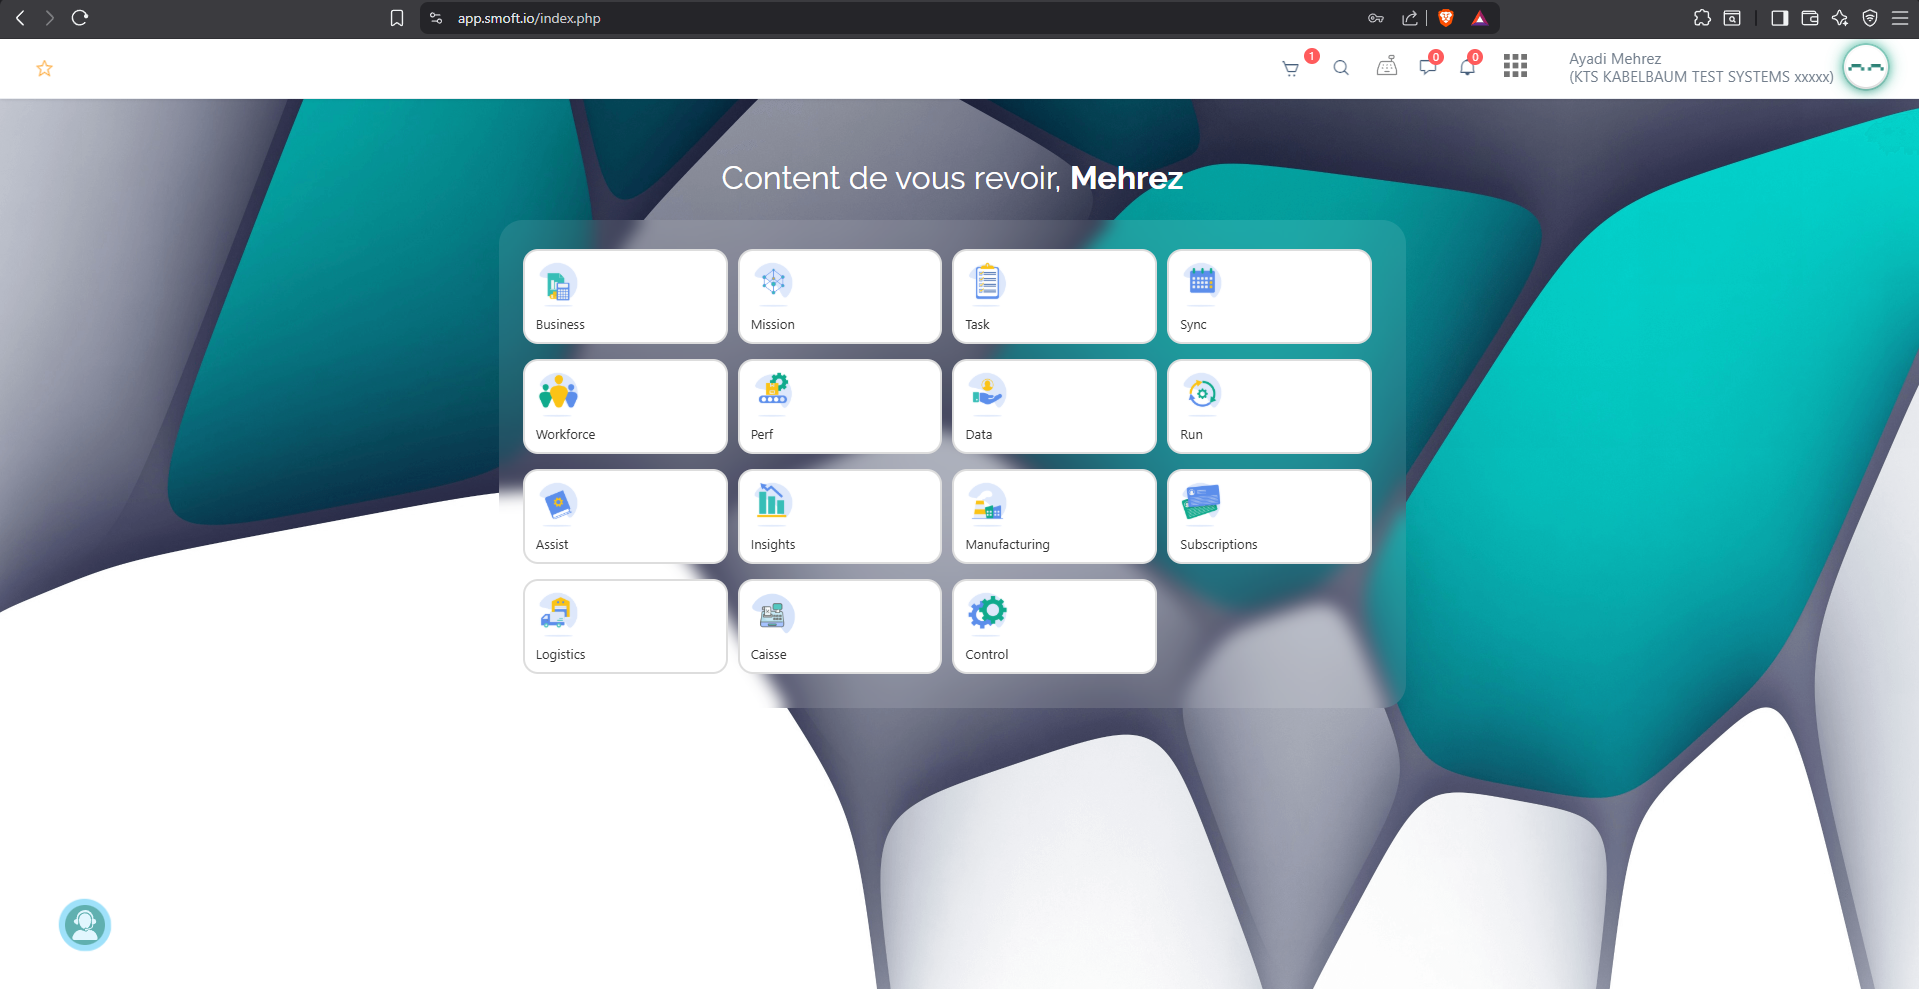
\includegraphics[width=12cm]{pictures/smoft-dashboard.png}
    \caption{SMOFT dashboard }
    \label{fig:smoft-dashboard}
\end{figure}
\subsubsection{SAP Digital Manufacturing}
SAP Digital Manufacturing is SAP's manufacturing execution and operations management solution. It connects shop-floor activities with enterprise planning, supports real-time production visibility, and helps manufacturing teams coordinate execution, traceability, and performance monitoring\hyperref[ref:SAPDM]{[6]}.

\begin{itemize}
    \item \textbf{Shop-floor coordination:} Supports execution of production activities directly from the manufacturing floor.
    \item \textbf{Real-time visibility:} Gives managers current information about ongoing production.
    \item \textbf{Traceability support:} Helps track production progress and operational events.
\end{itemize}

\textbf{Weak points:}
\begin{itemize}
    \item Deployment and integration can be complex for a small or medium company.
    \item The solution may require significant configuration and user training.
    \item It can be more expensive and heavier than a focused platform built for KTS-specific needs.
\end{itemize}

\begin{figure}[H]
    \centering
    
\includegraphics[width=4cm]{pictures/SAP DigitalManufacturing Logo.jpg}
    \caption{SAP Digital Manufacturing  \hyperref[ref:SAPDM-LOGO]{[7]}}
    \label{fig:sap-logo}
\end{figure}

\begin{figure}[h]
    \centering
    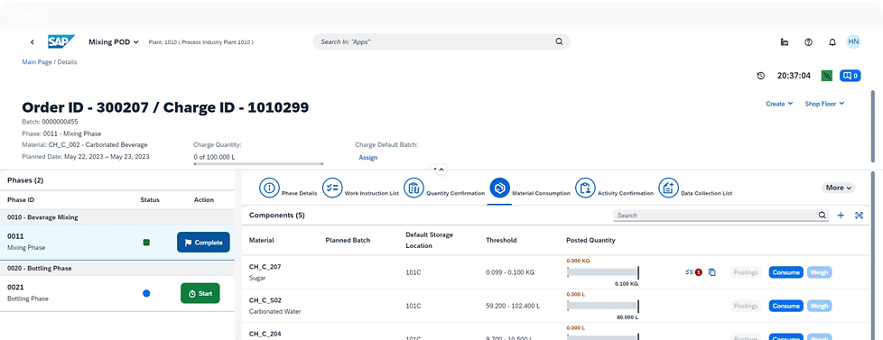
\includegraphics[width=12cm]{pictures/sap-dashboard.png}
    \caption{SAP Digital Manufacturing dashboard \hyperref[ref:SAPDM-DASHBOARD]{[8]}}
    \label{fig:sap-dashboard}
\end{figure}
\subsection{Proposed Solution}

Two alternatives were considered:

\subsubsection*{Alternative 1: degital logbook system}
Deploy a simple digital logbook system to replace paper forms while maintaining existing workflows. This approach minimizes disorder but can't improve processes that much.

\subsubsection*{Alternative 2:Production Management Platform}
Develop a web-based application that standardizes workflows,
offers role-based access control,
provides real-time production visibility,
and integrates inventory management.


\vspace{0.5cm}


The chosen approach is Alternative 2,
a comprehensive platform,
because it addresses not only the paper based process but also provide other solutions for better production managment. The implementation includes:

\begin{itemize}
    \item \textbf{centralized Tracking:} A unified platform where all work orders and tasks are digitally recorded.
    \item \textbf{Real-Time Visibility:} Administrators and workers access current status immediately, reducing communication delays.
    \item \textbf{Role-Based access:} Tailored interfaces and permissions for administrators, production workers.
    \item \textbf{Integrated inventory:} Stock management features linked directly to work orders, with reservation updates.
    \item \textbf{Chat messaging:} communication tool for better visibility and understanding.
    \item \textbf{Scalability:} A web-based architecture that grows with the company's production volume without the increase of manual efforts.
\end{itemize}
This solution is the best approache cause it solves a lot of linmitations and helps the company to grow efficiently.

The table \ref{tab:comparison} summarizes the comparison between the existing solutions and our project:
\begin{table}[H]
    \centering
    \caption{Comparison of Existing Solutions with Our Project} \label{tab:comparison}
    \renewcommand{\arraystretch}{1.2}
    \small
    \begin{tabularx}{\textwidth}{|p{3.6cm}|>{\raggedright\arraybackslash}X|>{\raggedright\arraybackslash}X|>{\raggedright\arraybackslash}X|}
        \hline
        \textbf{Criterion} & \textbf{SMOFT ERP} & \textbf{SAP Digital Manufacturing} & \textbf{Our project} \\
        \hline
        Traceability & Basic transactional traceability across business modules. & Strong production traceability for shop-floor operations. & Full traceability from work orders to stages, stock, notes, and chat. \\
        \hline
        Real-time visibility & Limited to ERP-level monitoring. & Good real-time production visibility. & Real-time visibility across production stages and inventory. \\
        \hline
        Role-based access & Available at business level, but not tailored to production roles. & Supports structured access for manufacturing users. & Dedicated access for administrators and production workers. \\
        \hline
        Usability for KTS & Too general for a dedicated production tracking workflow. & Powerful but heavier than required. & Designed specifically for KTS production tracking needs. \\
        \hline
        Deployment effort & Moderate, depending on customization. & High integration and configuration effort. & Lower effort because it is focused on the exact workflow. \\
        \hline
        Fit for KTS & Partial fit. & Partial fit, but more complex than necessary. & Best fit because it matches the company's process and constraints. \\
        \hline
    \end{tabularx}
\end{table}



\section{Work Methodology}

\subsection{Agile Scrum Method}

\hyperref[ref:scrumguide]{[9]} Scrum is a lightweight framework that helps people,
 teams and organizations generate value through adaptive solutions for complex problems.

In a nutshell, Scrum requires a Scrum Master to foster an environment where:

\begin{itemize}
    \item \textbf{1-} A Product Owner orders the work for a complex problem into a Product Backlog
    \item \textbf{2-} The Scrum Team turns a selection of the work into an Increment of value during a Sprint.
    \item \textbf{3-} The Scrum Team and its stakeholders inspect the results and adjust for the next Sprint.
    \item \textbf{4-} Repeat
\end{itemize}
During this project, \textbf{ Mr. Ayadi Mahrez} served as the Product Owner and Scrum Master to ensure that there was supervision in the project, prioritization of requirements, and management of the Scrum process. The members of the Scrum Team comprised only me as the developer of the application


\begin{figure}[H]
    \centering
    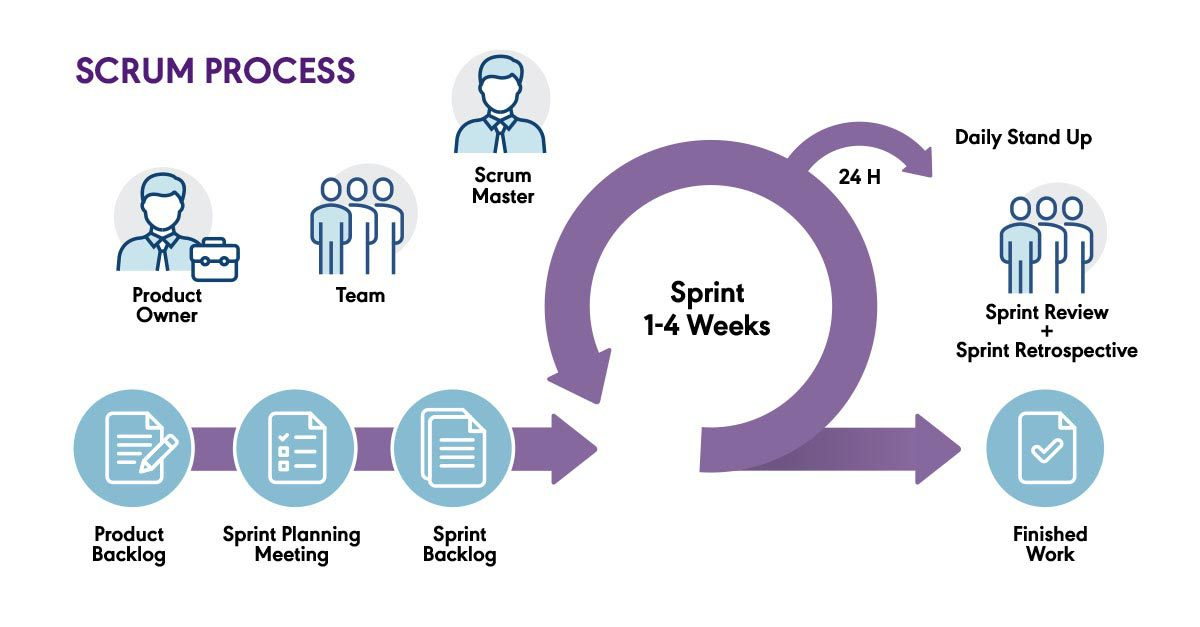
\includegraphics[width=12cm]{pictures/Scrum-methodology.jpg}
    \caption{SCRUM Process \hyperref[ref:scrum-Process]{[10]}}
    \label{fig:scrum-method}
\end{figure}

\section{Methodology: Scrum Sprint Summary}

Five sprints were carried out using the Scrum methodology to implement a usable increment of the production Tracker platform in each step.
The table \ref{tab:sprint-summary} summarizes the objectives and goals of each sprint.

\begin{table}[H]
    \caption{Task by Scrum Sprint} \label{tab:sprint-summary}
    \begin{tabular}{|p{1.5cm}|p{5.5cm}|p{7cm}|}
        \hline
        \textbf{Sprint} & \textbf{Objective} & \textbf{Goals} \\
        \hline
        1 & Foundation and Access \newline Control &  Establish authentication, \newline authorization, and a stable user management foundation\\
        \hline
        2 & Work Orders and Stage \newline Tracking & Enable the core production workflow from work order creation to stage history. \\
        \hline
        3 & Stock Management & Deliver a usable stock management system with validation and reliable inventory rules along with reservation functionality.\\
        \hline
        4 & Notes, Real-Time Chat,  and Notifications & Improve traceability and keep users informed in real time using communication and notification tools \\
        \hline
        5 & QR Codes, Analytics, and AI Reporting & Add communication, quick access, and managerial visibility  \\
        \hline
    \end{tabular}
\end{table}
\vspace{1cm}
\section*{Conclusion}

the overall project enviroment has been described in this chapter. Where we presented the context of our project,
starting with an introduction to the host organization and its activities,
then we studied the existing process and solutions, which leed us to identify limitations and weaknesses of the current system and propose the best solution,
finally we presented the work methodology where we did an even distribution of roles and priorities, next chapter will be about the analysis and the specification of requirements.


% Chapter 2: Analysis and Technical Specifications
\chapter{Analysis and Specification of requirements}

\newcommand{\chaptertwosoftwarefigure}[3]{%
\begin{figure}[H]
    \centering
    \includegraphics[width=0.45\textwidth,keepaspectratio]{#1}
    \caption{#2}
    \label{#3}
\end{figure}
}

\section{Introduction}
\label{sec:intro-analysis}

this chapter will present the analysis and specification of requirements used to develop this project, 
first we will identify the actors along with the functional and non-functional specifications,
then we will present the technical requirements including the software environment , 
finally we will present the global use case diagram, class diagram and the product backlog.
\section{Specification of requirements}


\subsection{actors identification}
the main actors of the system are:
\begin{itemize}
    \item \textbf{Administrators:} Responsible for managing the production process, assigning tasks, and overseeing operations.
    \item \textbf{Workers:} Execute assigned tasks, update work order statuses, and communicate with administrators.
\end{itemize}  




\subsection{Functional Specifications}


\subsubsection{User and Authentication Management}
The System shall:
\begin{itemize}
    \item provide secure user authentication with username and password.
    \item implement role-based access control (Admin, Worker).
    \item support user session management with token-based authentication.
    \item allow administrators to manage user accounts.
\end{itemize}

\subsubsection{Stock Management}
The System shall:
\begin{itemize}
    \item keep record of inventory items with unique identifiers.
    \item maintain stock levels and provide low-inventory alerts.
    \item record stock movement history and reservations.
\end{itemize}

\subsubsection{Work Order Management}
The System shall:
\begin{itemize}
    \item allow creation and assignment of work orders to workers.
    \item track work order status through different stages.
    \item generate QR codes for work orders for easy search.
\end{itemize}

\subsubsection{Chat and Communication}
The System shall:
\begin{itemize}
    \item provide real-time messaging between users.
    \item support file attachments in chat messages
    \item maintain message history and conversation threads
    \item implement chat notifications for new messages
\end{itemize}

\subsubsection{Notification System}
The System shall:
\begin{itemize}
    \item notify users of work order assignments in real-time
    \item alert users to inventory status changes
    \item provide notifications for chat messages .
\end{itemize}

\subsubsection{Production Stages}
The System shall:
\begin{itemize}
    \item define production stages and workflows
    \item track stage progression and duration
    \item assign workers to specific production stages
\end{itemize}

\subsection{Non-Functional Specifications}
\label{sec:non-functional-specs}

\subsubsection{Performance Requirements}

\begin{itemize}
    \item System shall respond to user requests within 2 seconds under normal load
    \item System shall support concurrent users up to 500 without performance degradation
    \item Real-time notifications shall be delivered within 1 second of triggering event
    \item Page load time shall not exceed 3 seconds for desktop and 4 seconds for mobile
\end{itemize}

\subsubsection{Scalability Requirements}

\begin{itemize}
    \item System architecture shall support horizontal scaling for increased load
    \item Database shall efficiently handle queries with up to 10 million records
    \item System shall support adding new features without major restructuring
\end{itemize}

\subsubsection{Security Requirements}

\begin{itemize}
    \item All user passwords shall be hashed using industry-standard algorithms
    \item User data shall be protected with proper access control mechanisms
    \item API endpoints shall require proper authentication and authorization
\end{itemize}
\subsubsection{Usability Requirements}

\begin{itemize}
    \item User interface shall follow modern UX/UI principles with consistent design
    \item System shall be accessible on desktop and mobile devices
    \item Navigation shall be intuitive requiring minimal training
    \item System shall provide clear error messages and help documentation
\end{itemize}

\subsubsection{Compatibility Requirements}

\begin{itemize}
    \item System shall be compatible with modern web browsers (Chrome, Firefox, Safari, Edge)
    \item System shall work on iOS and Android mobile devices
    \item Backend APIs shall be independent of frontend implementation
\end{itemize}
\subsection{Technical Requirements Specification}

The software environment was organized around the technologies used to build, run, and maintain the platform.
Each tool is presented by its logo and description below in the table \ref{tab:chapter2-software-environment}.

\renewcommand{\arraystretch}{1.35}
\small
\begin{longtable}{|p{0.20\textwidth}|p{0.72\textwidth}|}
    \caption{Software environment technologies used}\label{tab:chapter2-software-environment}\\
    \hline
    \textbf{Logo} & \textbf{Description} \\
    \hline
    \endfirsthead

    \hline
    \textbf{Logo} & \textbf{Description} \\
    \hline
    \endhead

    \hline
    \endfoot

    \hline
    \begin{center}
\includegraphics[width=0.14\textwidth,keepaspectratio]{pictures/next js logo.png}\end{center} & \textbf{Next.js}\newline According to the official documentation, Next.js is a React framework for building full-stack web applications. It provides routing, rendering strategies, and built-in optimizations while automatically configuring lower-level tooling. This helped us build the frontend faster with a clear project structure and production-ready defaults \hyperref[ref:nextjs]{[11]}. \\
    \hline
    \begin{center}
\includegraphics[width=0.14\textwidth,keepaspectratio]{pictures/Node.js_logo.svg.png}\end{center} & \textbf{Node.js}\newline Node.js is officially presented as a free, open-source, cross-platform JavaScript runtime environment. It allows developers to create servers, web applications, command-line tools, and scripts with JavaScript. In this project, it provided the execution environment for backend services and API logic \hyperref[ref:nodejs]{[12]}. \\
    \hline
    \begin{center}
\includegraphics[width=0.14\textwidth,keepaspectratio]{pictures/Expressjs.png}\end{center} & \textbf{Express}\newline The Express official site describes it as a fast, unopinionated, minimalist web framework for Node.js. It offers a flexible routing and middleware model with essential features for web and mobile APIs. We used Express to implement REST endpoints, middleware pipelines, and role-protected routes \hyperref[ref:express]{[13]}. \\
    \hline
    \begin{center}
\includegraphics[width=0.14\textwidth,keepaspectratio]{pictures/PostgreSQL-Logo.png}\end{center} & \textbf{PostgreSQL}\newline PostgreSQL is described by its official project as a powerful, open-source object-relational database system. It is recognized for reliability, data integrity, SQL support, and extensibility for complex workloads. In our platform, PostgreSQL stores users, work orders, stock records, notifications, and chat data \hyperref[ref:postgresql]{[14]}. \\
    \hline
    \begin{center}
\includegraphics[width=0.14\textwidth,keepaspectratio]{pictures/prisma-logo.png}\end{center} & \textbf{Prisma ORM}\newline Prisma ORM is documented as a next-generation ORM for Node.js and TypeScript that provides type-safe database access. Its toolkit includes Prisma Client, Prisma Migrate, and Prisma Studio for querying, migrations, and data inspection. We used Prisma as the main data access layer to keep schema evolution and queries maintainable \hyperref[ref:prisma]{[15]}. \\
    \hline
    \begin{center}
\includegraphics[width=0.14\textwidth,keepaspectratio]{pictures/socket io-logo.png}\end{center} & \textbf{Socket.IO}\newline Socket.IO is officially introduced as a library for low-latency, bidirectional, event-based communication. It supports transport fallback and includes features such as automatic reconnection and event acknowledgements. This was essential for real-time chat updates and immediate notification delivery in the application \hyperref[ref:socketio]{[16]}. \\
    \hline
    \begin{center}
\includegraphics[width=0.14\textwidth,keepaspectratio]{pictures/vscode-logo.png}\end{center} & \textbf{Visual Studio Code}\newline The official VS Code website presents it as an open-source AI code editor and a world-class editor core used by millions of developers. It provides extension support, integrated terminal, debugging features, and rich language tooling. It was our primary development environment for frontend and backend implementation tasks \hyperref[ref:vscode]{[17]}. \\
    \hline
    \begin{center}
\includegraphics[width=0.14\textwidth,keepaspectratio]{pictures/Diagrams.net_Logo.svg.png}\end{center} & \textbf{diagram.net}\newline diagrams.net (previously \textbf{draw.io}) is a graph drawing application written in JavaScript. It can be used to design and export many kinds of diagrams, including circuit diagrams, floor plans, flowcharts, infographics, mind maps, and UML designs. \hyperref[ref:diagramsnet]{[18]}. \\
    \hline
    \begin{center}
\includegraphics[width=0.14\textwidth,keepaspectratio]{pictures/Latex logo.png}\end{center} & \textbf{LaTeX}\newline LaTeX is a high-quality typesetting system; it includes features designed for the production of technical and scientific documentation. LaTeX is the de facto standard for the communication and publication of scientific documents \hyperref[ref:latex]{[19]}. \\
    \hline
\end{longtable}
\vspace{2cm}
\section{Global use case diagramm}

the figure \ref{fig:chapter2-use-case-diagram} illustrates the global use case diagram of the system, which represents the interactions between the actors and the main functionalities of the platform. 
\begin{figure}[H]
    \centering
    
    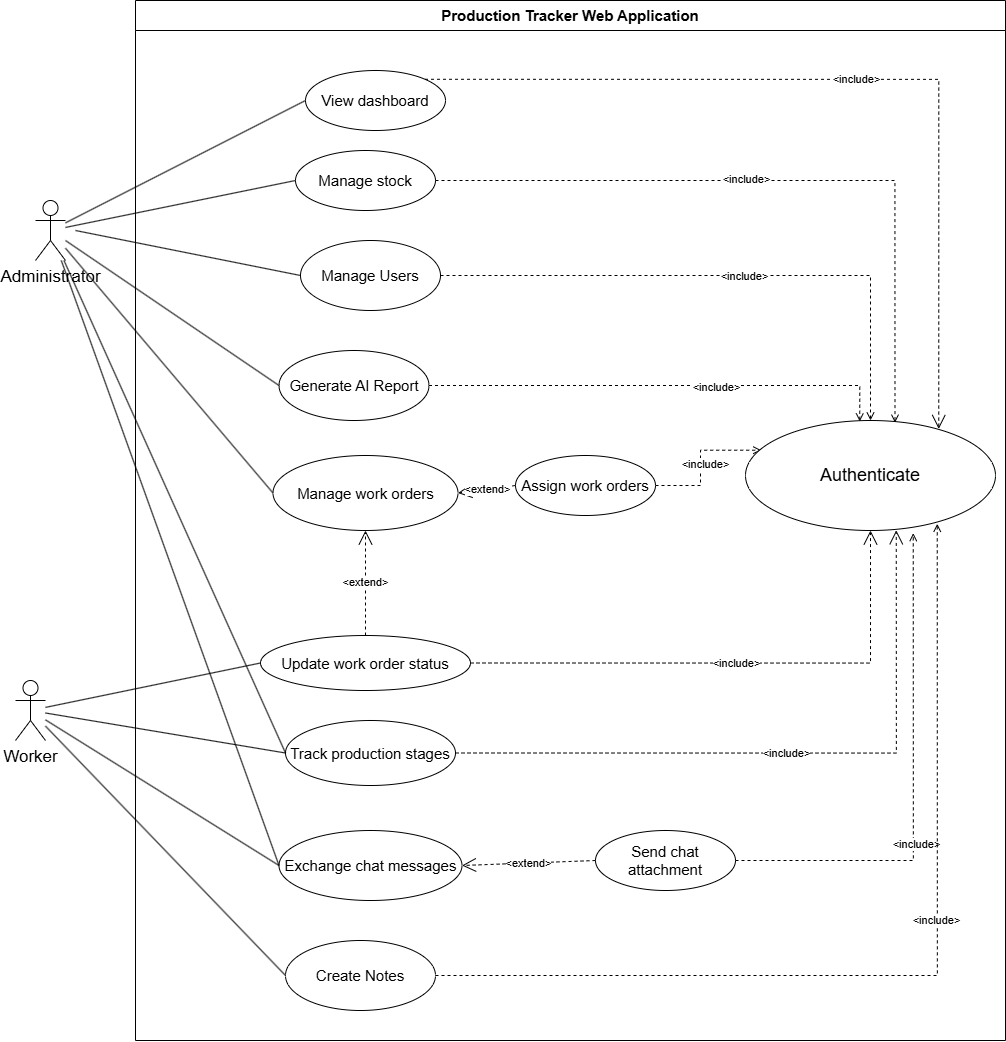
\includegraphics[width=\textwidth,keepaspectratio]{pictures/use caseFinal.drawio.png}
    \vspace*{\fill}
    \caption{Use Case Diagram}
    \label{fig:chapter2-use-case-diagram}
\end{figure}
\section{Global class diagramm}
the figure \ref{fig:chapter2-class-diagram} illustrates the global class diagram of the system.
\begin{sidewaysfigure}
    \centering
    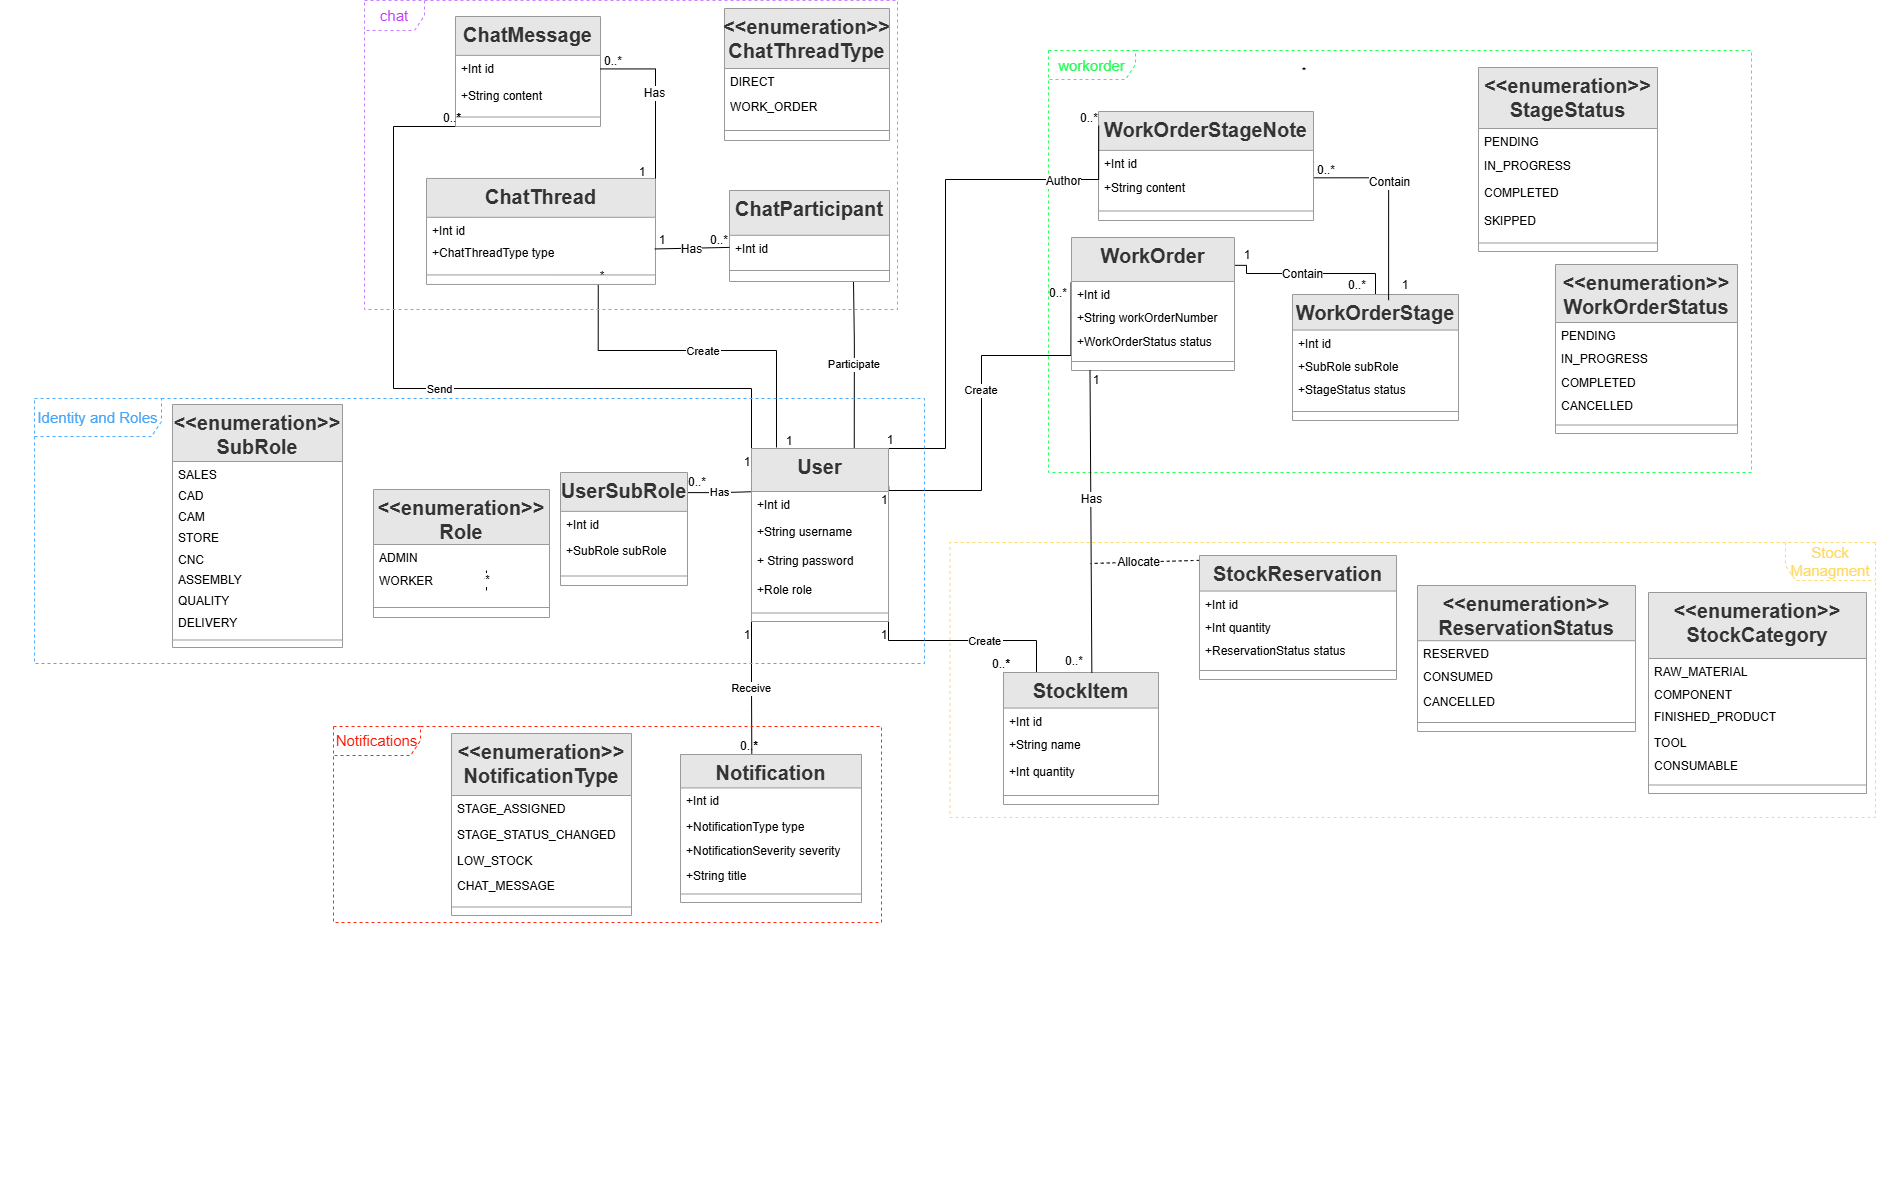
\includegraphics[width=0.95\textheight]{pictures/Class Diagram2.drawio.png}
    \caption{Global class diagram}
    \label{fig:chapter2-class-diagram}
\end{sidewaysfigure}
\section{Planning}
\subsection{Product backlog}
in this section we present the product backlog, which is a prioritized list of features and requirements that will guide the development process. Each item in the backlog is defined as a user story, which describes a specific functionality from the perspective of the end user. The backlog is organized into sprints, with each sprint focusing on a set of related features that will be developed and delivered together. The Table \ref{tab:product-backlog} represents the global Product backlog.
\footnotesize
\begin{longtable}{|p{0.08\textwidth}|p{0.24\textwidth}|p{0.48\textwidth}|p{0.14\textwidth}|}
    \caption{Product backlog}\label{tab:product-backlog}\\
    \hline
    \textbf{ID} & \textbf{Fonctionality} & \textbf{User Story} & \textbf{Actor} \\
    \hline
    \endfirsthead

    \hline
    \textbf{ID} & \textbf{Fonctionality} & \textbf{User Story} & \textbf{Actor} \\
    \hline
    \endhead

    \hline
    \endfoot

    \hline
    \multicolumn{4}{|l|}{\textbf{Sprint 1: Foundation and Access Control}} \\
    \hline
    PB-01 & User Authentication & As an administrator, I want to log in securely so that I can access protected management features. & Administrator \\
    \hline
    PB-02 & Role-Based Access Control & As an administrator, I want role-based permissions so that users only access features related to their role. & Administrator \\
    \hline
    PB-03 & User Management & As an administrator, I want to create, update, and deactivate user accounts so that I can manage the team effectively. & Administrator \\
    \hline
    PB-04 & Session Security & As a user, I want secure session handling with token expiration so that my account remains protected. & Administrator / Worker \\
    \hline
    \multicolumn{4}{|l|}{\textbf{Sprint 2: Work Orders and Stage Tracking}} \\
    \hline
    PB-05 & Work Order Creation & As an administrator, I want to create work orders with required details so that production tasks are clearly defined. & Administrator \\
    \hline
    PB-06 & Work Order Assignment & As an administrator, I want to assign work orders to workers so that each task has a responsible person. & Administrator \\
    \hline
    PB-07 & Work Order Status Tracking & As a worker, I want to update the status of my assigned work orders so that progress is visible to the administrator in real time. & Worker \\
    \hline
    \multicolumn{4}{|l|}{\textbf{Sprint 3: Stock Management}} \\
    \hline
    PB-08 & Inventory Registration & As an administrator, I want to register stock items with unique identifiers so that materials can be tracked accurately. & Administrator \\
    \hline
    PB-09 & Stock Reservation & As a worker, I want to reserve stock items for my tasks and mark them as consumed when used. & Worker \\
    \hline
    PB-10 & Reservation Tracking & As an administrator, I want to monitor stock reservations so that inventory usage is auditable. & Administrator \\
    \hline
    \multicolumn{4}{|l|}{\textbf{Sprint 4: Notes and Notifications (Real-Time Chat included)}} \\
    \hline
    PB-11 & Stage Notes & As a worker, I want to add notes on work stages so that operational details are documented for traceability. & Worker \\
    \hline
    PB-12 & Notification Center & As a user, I want to receive notifications for assignments, updates, and messages so that I do not miss important events. & Administrator / Worker \\
    \hline
    PB-13 & Real-Time Chat & As a user, I want to chat with other users in real time so that I can discuss issues and coordinate. & Worker / Administrator \\
    \hline
    PB-14 & File Sharing in Chat & As a user, I want to attach files in chat so that I can share production documents and evidence. & Administrator / Worker \\
    \hline
    \multicolumn{4}{|l|}{\textbf{Sprint 5: QR Codes, Analytics, and AI Reporting}} \\
    \hline
    PB-15 & QR Code Generation & As an administrator, I want generated QR codes for work orders so that identification is faster. & Administrator \\
    \hline
    PB-16 & QR Code Scanning & As a user, I want to scan QR codes so that I can quickly search and access work orders. & Worker / Administrator \\
    \hline
    PB-17 & AI Reporting Engine & As an administrator, I want AI-assisted reporting so that I can make faster data-driven decisions. & Administrator \\
    \hline
    PB-18 & Analytics Dashboard & As an administrator, I want an analytical dashboard for production data so that I can monitor KPIs and trends. & Administrator \\
    \hline
\end{longtable}
\normalsize
\subsection{Sprint Planning}

The internship lasted three and a half months, so the sprint planning was distributed accordingly.

The table \ref{tab:sprint-plan} summarizes the sprint plan by priority and period.

\begin{table}[H]
    \centering
    \caption{Sprint Plan} \label{tab:sprint-plan}
    \label{tab:sprint-planning}
    \begin{tabular}{|p{2.8cm}|p{4.6cm}|p{2.2cm}|p{2.6cm}|}
        \hline
         & \textbf{Sprint} & \textbf{Priority} & \textbf{Period} \\
        \hline
        \multirow{3}{*}{Release 1} & Foundation and Access Control & 1 & 21 days \\
        \cline{2-4}
         & Work Orders and Stage Tracking & 2 & 21 days \\
        \cline{2-4}
         & Stock Management & 3 & 21 days \\
        \hline
        \multirow{2}{*}{Release 2} & Notes and Notifications & 4 & 21 days \\
        \cline{2-4}
         & Real-Time Chat, QR Codes, AI Reporting & 5 & 21 days \\
        \hline
    \end{tabular}
\end{table}


\section{Conclusion}
\label{sec:conclusion-analysis}
This chapter provided a detailed analysis and specification of the requirements for the production tracking platform.Throughout this chapter, We identified the main actors involved in the system, 
defined functional and non-functional specifications to make sure the platform meets the company's needs,
outlined the technical environment,
In addition, we created several UML diagrams, including use case and class diagrams to provide a clear understanding of the system's behavior.
Finally The detailed product backlog will serve as a roadmap for the development process and will guide the implementation of the platform.
in the next chapter, we will start the implementation of the first release, which focuses on the development of the first three sprints.    

% Chapter 3: System Design
\chapter{Release 1}
\label{chap:release1}

\section{Introduction}
\label{sec:release1-intro}

Release 1 presents the first three sprints of the Production Tracker project, focusing on building a solid foundation with authentication and access control, implementing the core production flow, and developing an inventory management system. This release provides the essential features needed to track work orders and manage stock efficiently.

\section{Sprint 1: Foundation and Access Control}
\label{sec:sprint1}

\subsection{Sprint 1 Backlog}
\label{sec:sprint1-backlog}
the table \ref{tab:sprint1-backlog} summarizes the user stories and tasks completed during Sprint 1.
\footnotesize
\begin{longtable}{|p{0.10\textwidth}|p{0.50\textwidth}|p{0.32\textwidth}|}
    \caption{Sprint 1 Backlog}\label{tab:sprint1-backlog}\\
    \hline
    \textbf{ID} & \textbf{User Story} & \textbf{Tasks} \\
    \hline
    \endfirsthead
    \hline
    \textbf{ID} & \textbf{User Story} & \textbf{Tasks} \\
    \hline
    \endhead
    \hline
    \endfoot
    PB-01 & As an administrator, I want to log in securely so that I can access protected features. & Setup authentication module; \newline   Implement login/logout; \newline Add password hashing \\
    \hline
    PB-02 & As an administrator, I want role-based permissions so that users access only appropriate features. & Define role models; \newline  Implement permission checks; \newline  Create role management UI \\
    \hline
    PB-03 & As an administrator, I want to create and manage user accounts so that the team can access the system. & Build user CRUD operations; \newline  Add user validation; \newline  Create user management interface \\
    \hline
    PB-04 & As a user, I want secure session handling so that my account remains protected. & Implement JWT tokens; \newline  Add session expiration; \newline  Create token refresh mechanism \\
    \hline
\end{longtable}
\normalsize
\subsection{Sprint 1 use case diagram}
the figure \ref{fig:sprint1-use-case-diagram} illustrates the main use cases implemented in Sprint 1, focusing on user authentication and management features. It shows the interactions between the administrator and the system for logging in, and managing user accounts.
\begin{figure}[H]
    \centering
    
    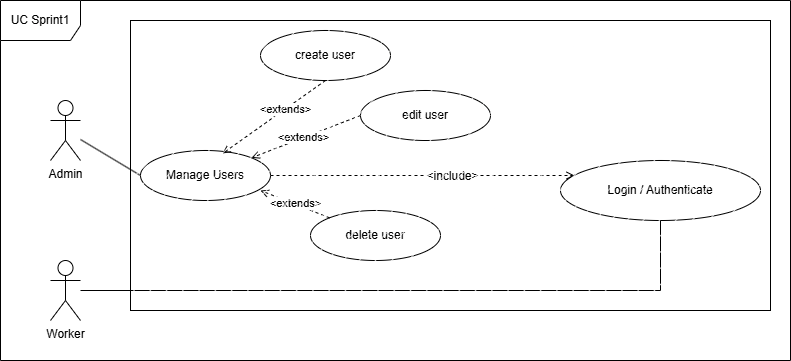
\includegraphics[width=\textwidth,keepaspectratio]{pictures/sprint1 use case diagarm.drawio.png}
    \vspace*{\fill}
    \caption{Sprint 1 Use Case Diagram}
    \label{fig:sprint1-use-case-diagram}
\end{figure}
\subsection{User Login and Protected Resource Access — JWT Sequence Diagram}
    JSON Web Token (JWT) is a proposed Internet standard for creating data with optional signature and/or optional encryption whose payload holds JSON that asserts some number of claims. The tokens are signed either using a private secret or a public/private key. \hyperref[ref:jwt]{[20]} 

the figure \ref{fig:jwt-sequence-diagram} illustrates the sequence of interactions during the authentication process using JWT tokens. 

\begin{figure}[H]
    \centering
    
    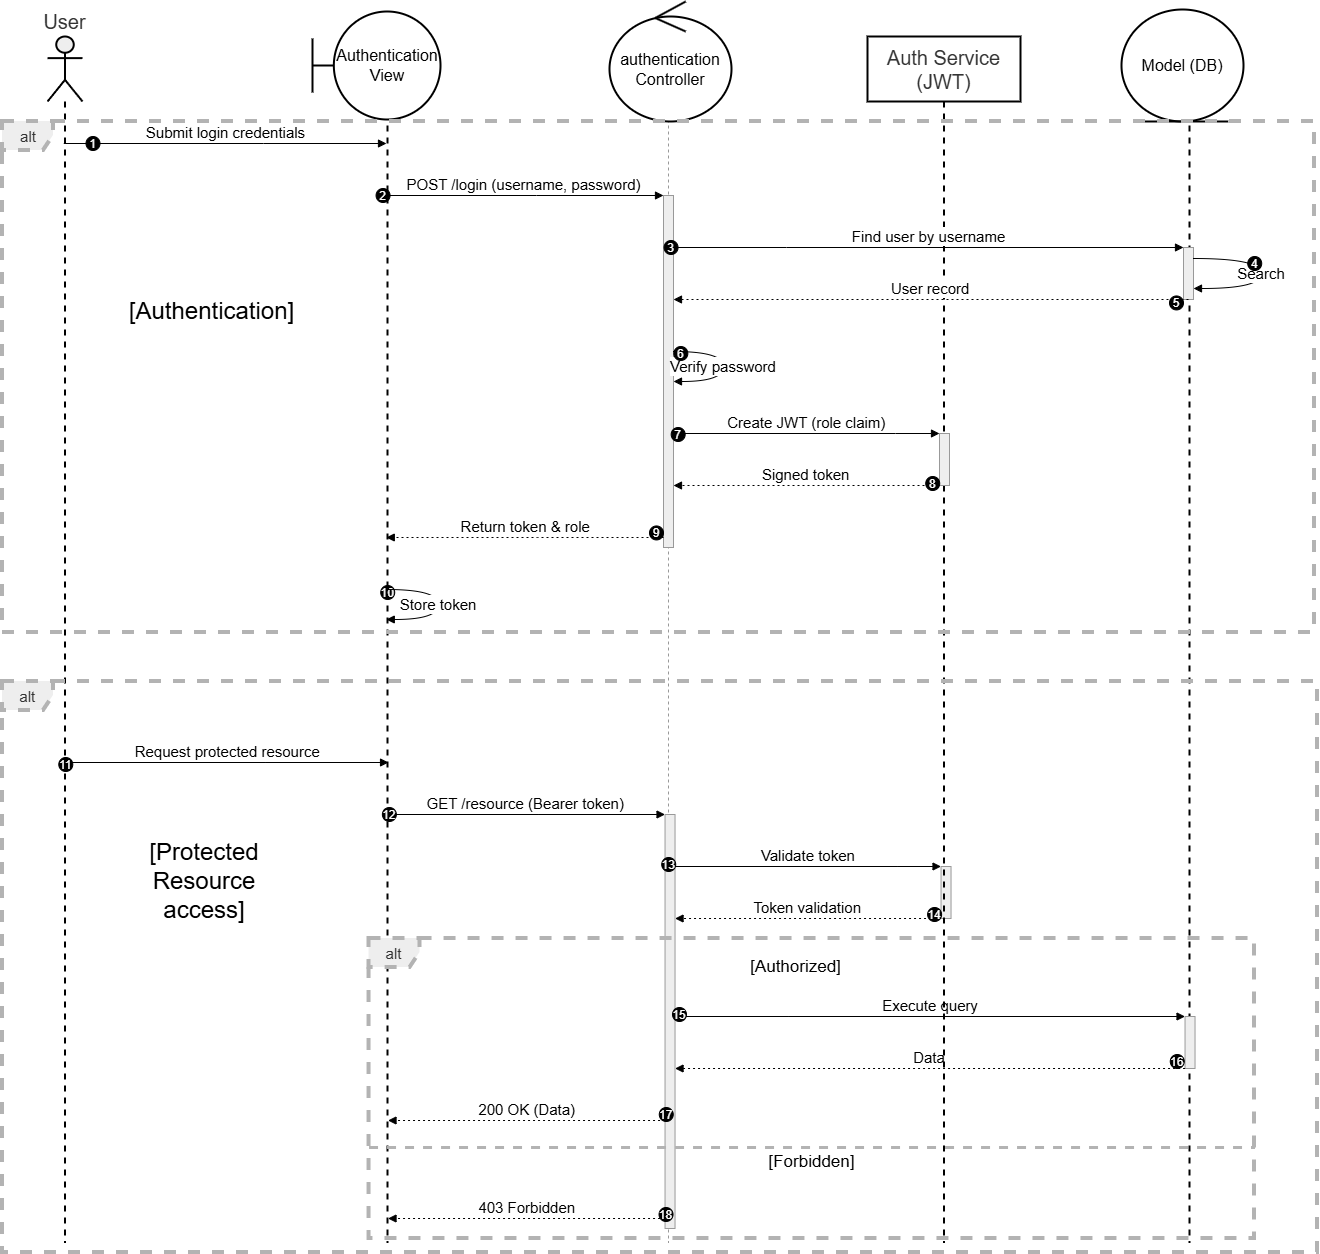
\includegraphics[width=\textwidth,keepaspectratio]{pictures/jwt authentication sequence diagram.drawio.png}
    \vspace*{\fill}
    \caption{Authentication Sequence Diagram}\label{fig:jwt-sequence-diagram}
\end{figure}


\subsection{Sprint 1: Application Interface Overview}
\label{sec:sprint1-interfaces}
The figure \ref{fig:login-interface} show the login interface that represents the gate to access the platform.
While the figures \ref{fig:user-management-interface} and \ref{fig:user-creation-modal} show the user management interface that allows administrators to create and manage user accounts, including a modal for creating new users with role assignments and validation features.
\begin{figure}[H]
    \centering
    
    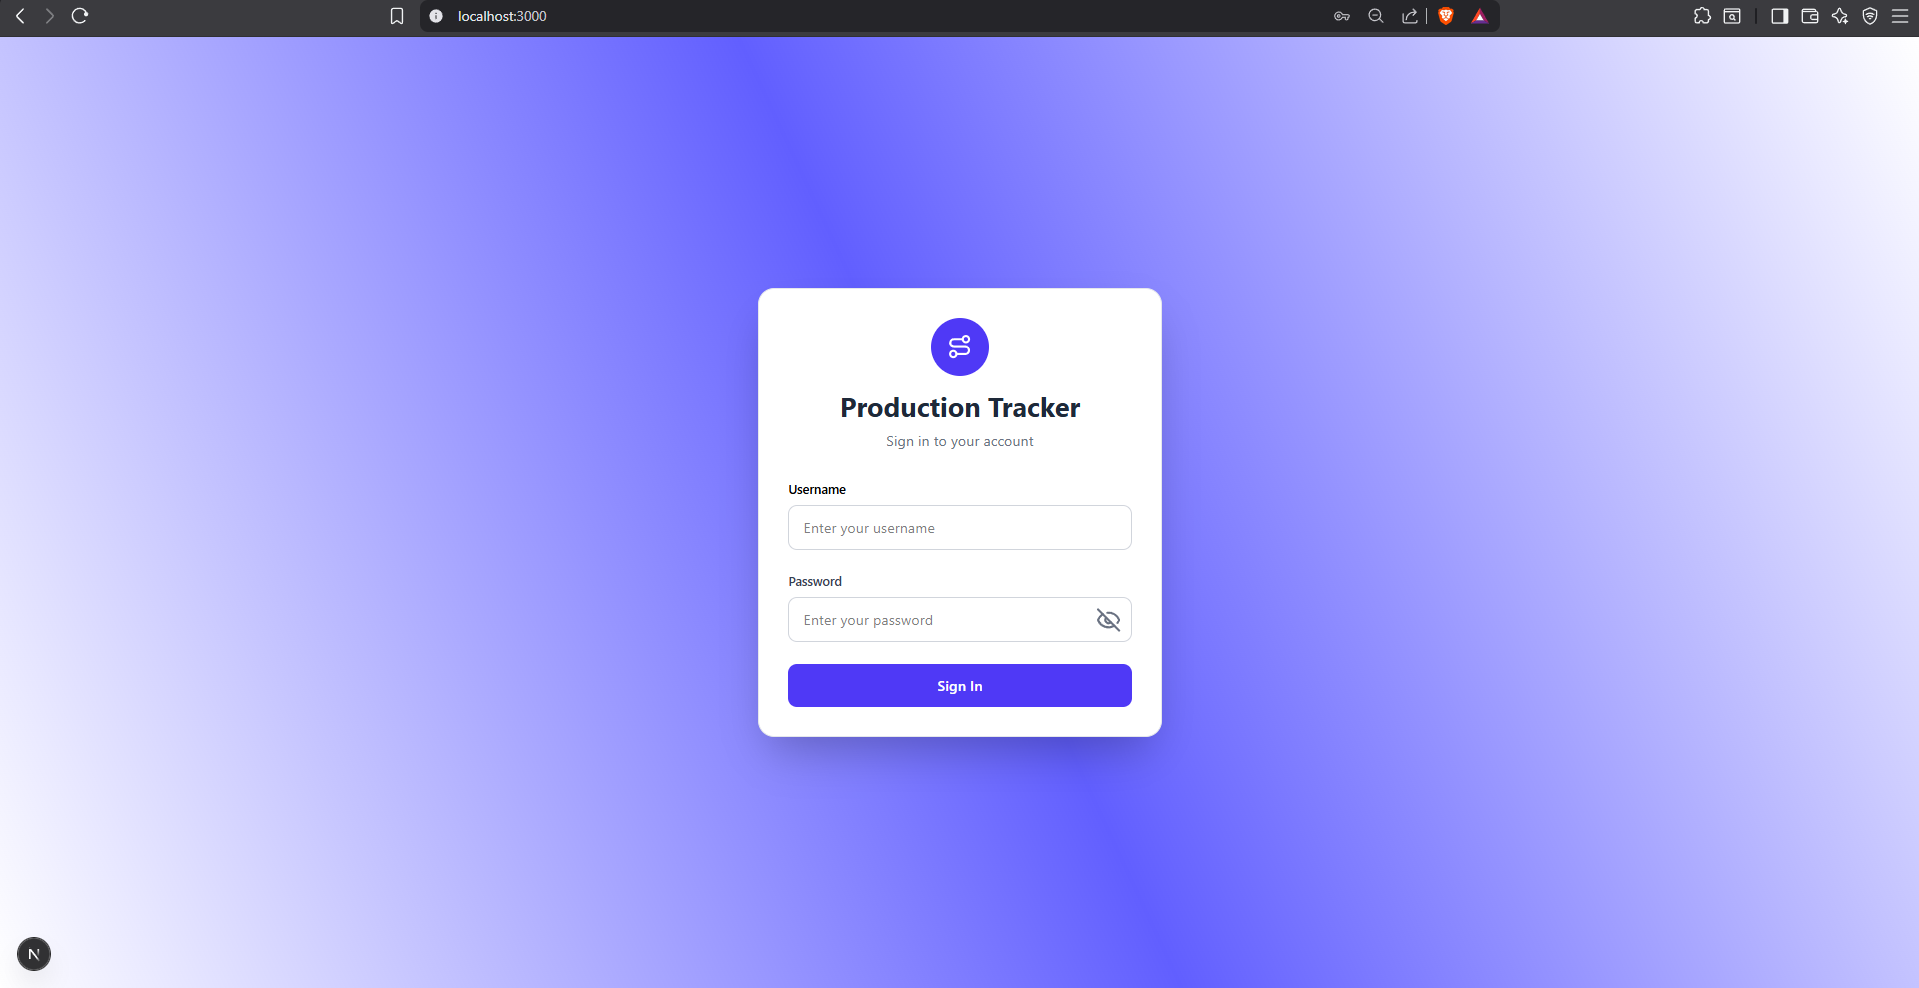
\includegraphics[width=\textwidth,keepaspectratio]{pictures/login-interface.png}
    \vspace*{\fill}
    \caption{Login Interface} \label{fig:login-interface}
\end{figure}
\begin{figure}[H]
    \centering

    \begin{minipage}[t]{0.48\textwidth}
        \centering
        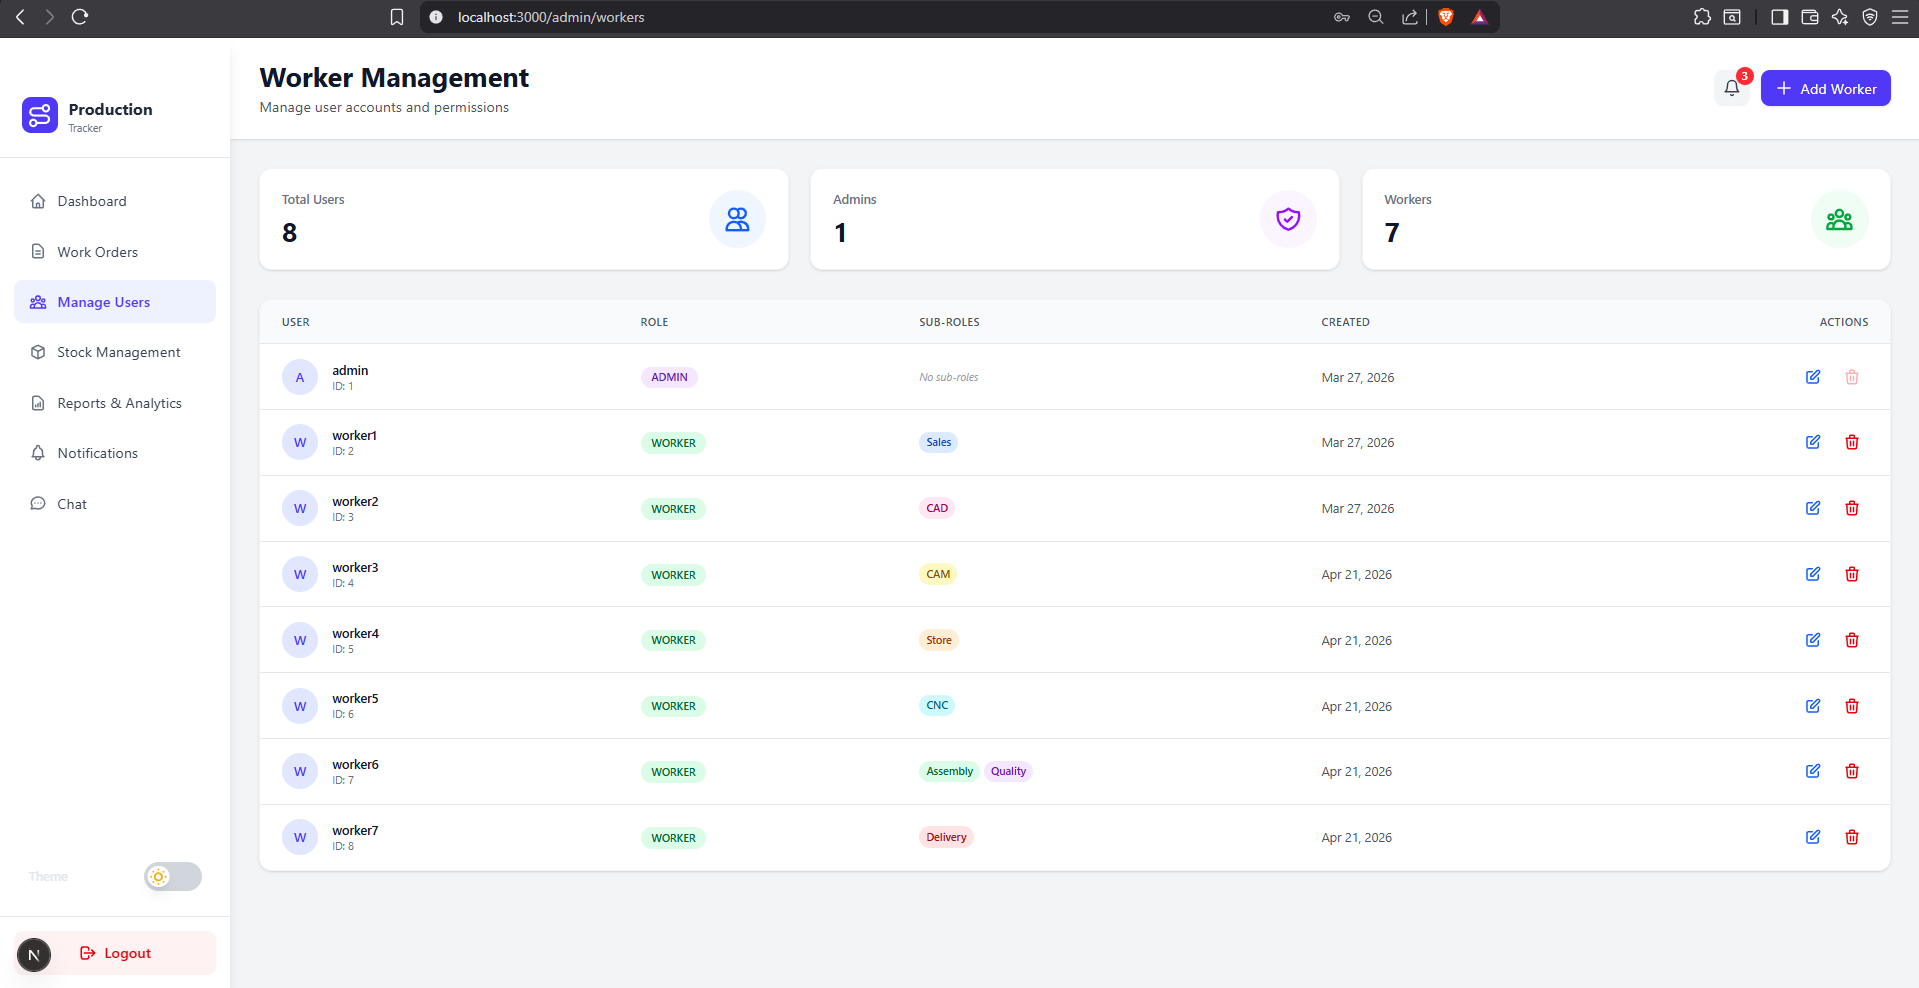
\includegraphics[width=\textwidth]{pictures/user managment interface.png}
        \caption{User Management Interface}
        \label{fig:user-management-interface}
    \end{minipage}
    \hfill
    \begin{minipage}[t]{0.48\textwidth}
        \centering
        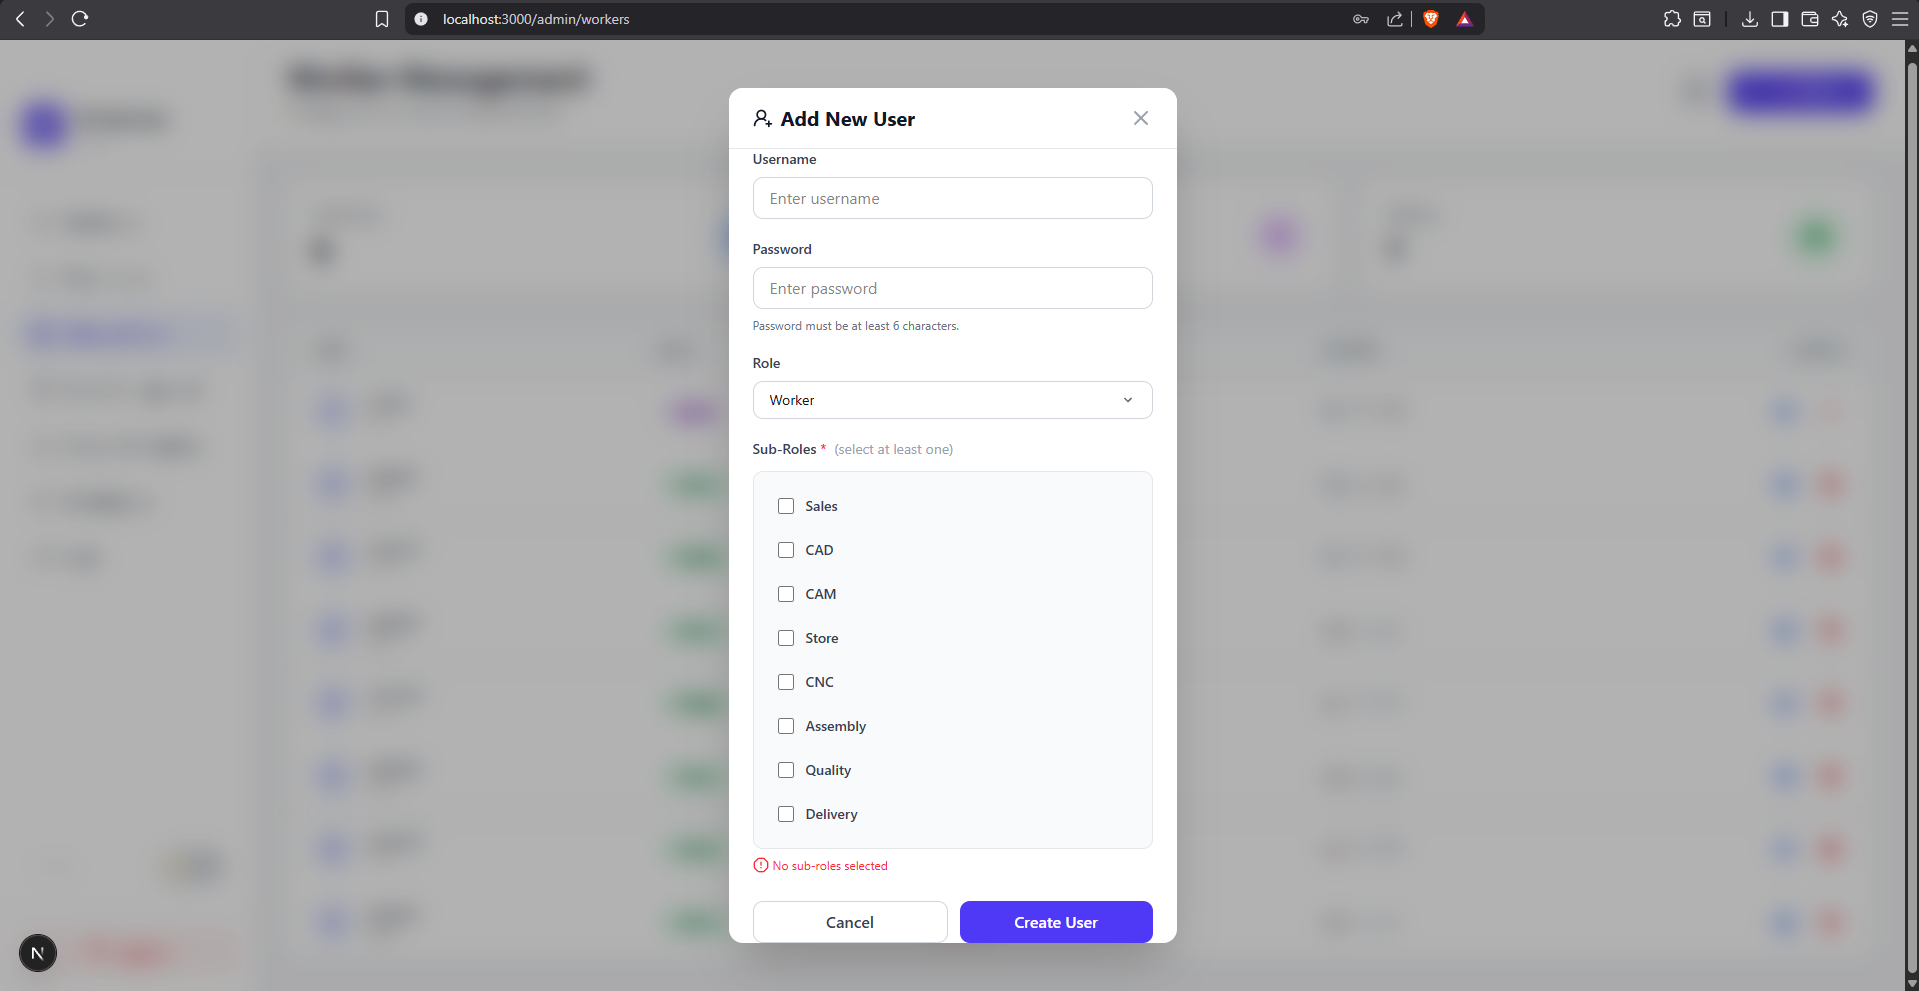
\includegraphics[width=\textwidth]{pictures/user creation modal.png}
        \caption{User Creation Modal}
        \label{fig:user-creation-modal}
    \end{minipage}

\end{figure}

\section{Sprint 2: Work Orders and Stage Tracking}
\label{sec:sprint2}

\subsection{Sprint Backlog}
\label{sec:sprint2-backlog}


the table \ref{tab:sprint2-backlog} summarizes the user stories and tasks completed during Sprint 2.
\begin{longtable}{|p{0.10\textwidth}|p{0.50\textwidth}|p{0.32\textwidth}|}
    \caption{Sprint 2 Backlog}\label{tab:sprint2-backlog}\\
    \hline
    \textbf{ID} & \textbf{User Story} & \textbf{Tasks} \\
    \hline
    \endfirsthead
    \hline
    \textbf{ID} & \textbf{User Story} & \textbf{Tasks} \\
    \hline
    \endhead
    \hline
    
    \endfoot
    
    PB-05 & As an administrator, I want to create work orders with all required details so that tasks are clearly defined. & Design work order schema; \newline  Build creation form; \newline  Add validation and error handling \\
    \hline
    PB-06 & As an administrator, I want to assign work orders to workers so that each task has a responsible person. & Create assignment workflow; \newline  Build assignment UI; \newline  Add notification trigger \\
    \hline
    PB-07 & As a worker, I want to update my work order status so that progress is visible in real time. & Build status update endpoints; \newline  Create status UI; \newline Add real-time updates \\
    \hline
\end{longtable}
\normalsize
\subsection{ Sprint 2 use case diagram}
the figure \ref{fig:sprint2-use-case-diagram} illustrates the main use cases implemented in Sprint 2, focusing on work order management and stage tracking features. It shows the interactions between the administrator and workers with the system for creating, assigning, and updating work orders.
\begin{figure}[H]
    \centering
    
    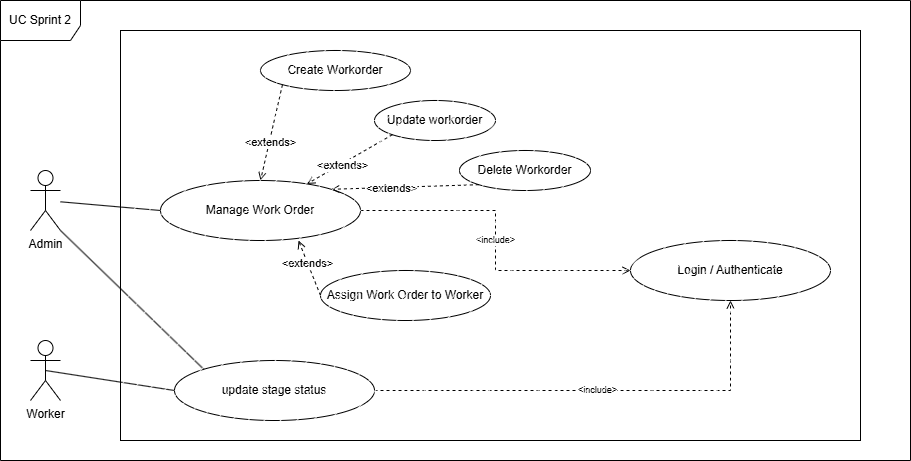
\includegraphics[width=\textwidth,keepaspectratio]{pictures/Sprint2 use case diagram.drawio.png}
    \vspace*{\fill}
    \caption{Sprint 2 Use Case Diagram}
    \label{fig:sprint2-use-case-diagram}
\end{figure}

\subsection{ Sequence Diagram for Work Order Progress Update}
the figure \ref{fig:work-order-sequence-diagram} illustrates the sequence of interactions during the work order progress update process, showing how a worker updates the status of a work order and how the system processes this update to reflect changes in the production workflow.
\begin{sidewaysfigure}
    \centering
    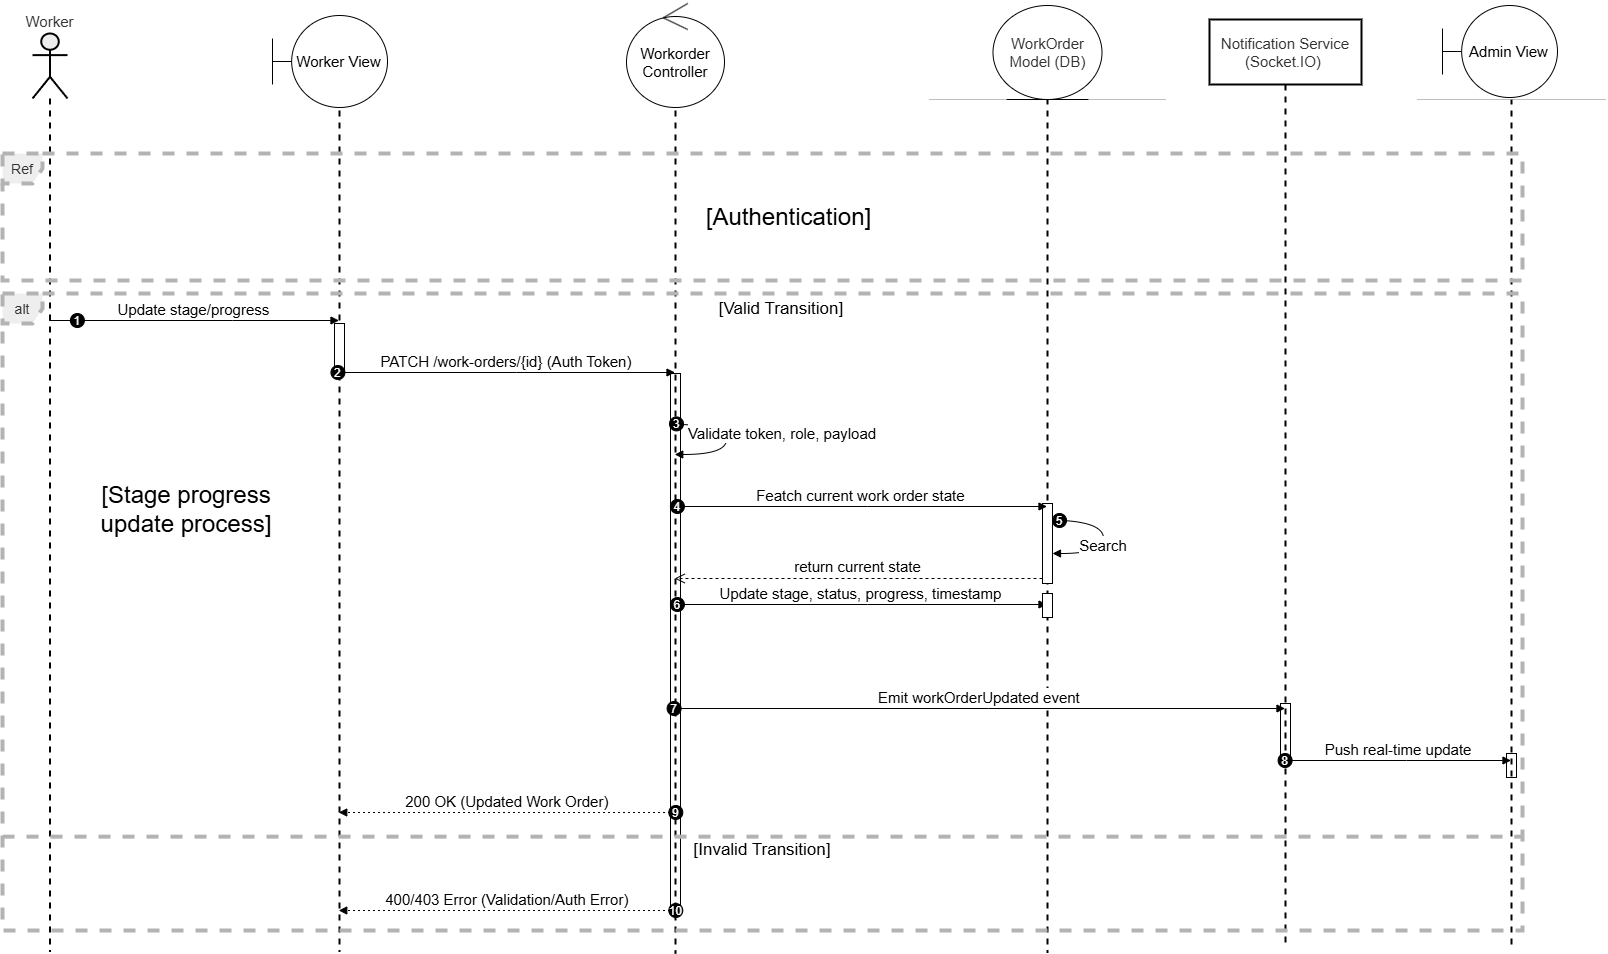
\includegraphics[width=0.95\textheight]{pictures/Work order stage_progress update.drawio.png}
    \caption{Work Order Progress Update Sequence Diagram}
    \label{fig:work-order-sequence-diagram}
\end{sidewaysfigure}

\subsection{Sprint 2: Application Interface Overview}
\label{sec:sprint2-interfaces}

the figures \ref{fig:work-order-management-interface}, \ref{fig:production-stages-admin}, and \ref{fig:worker-tasks-view} show the interfaces related to work order management, production stages administration, and worker task views, respectively. These interfaces allow administrators to manage work orders and production stages while providing workers with a clear view of their assigned tasks and progress.
\begin{figure}[H]
    \centering
    
    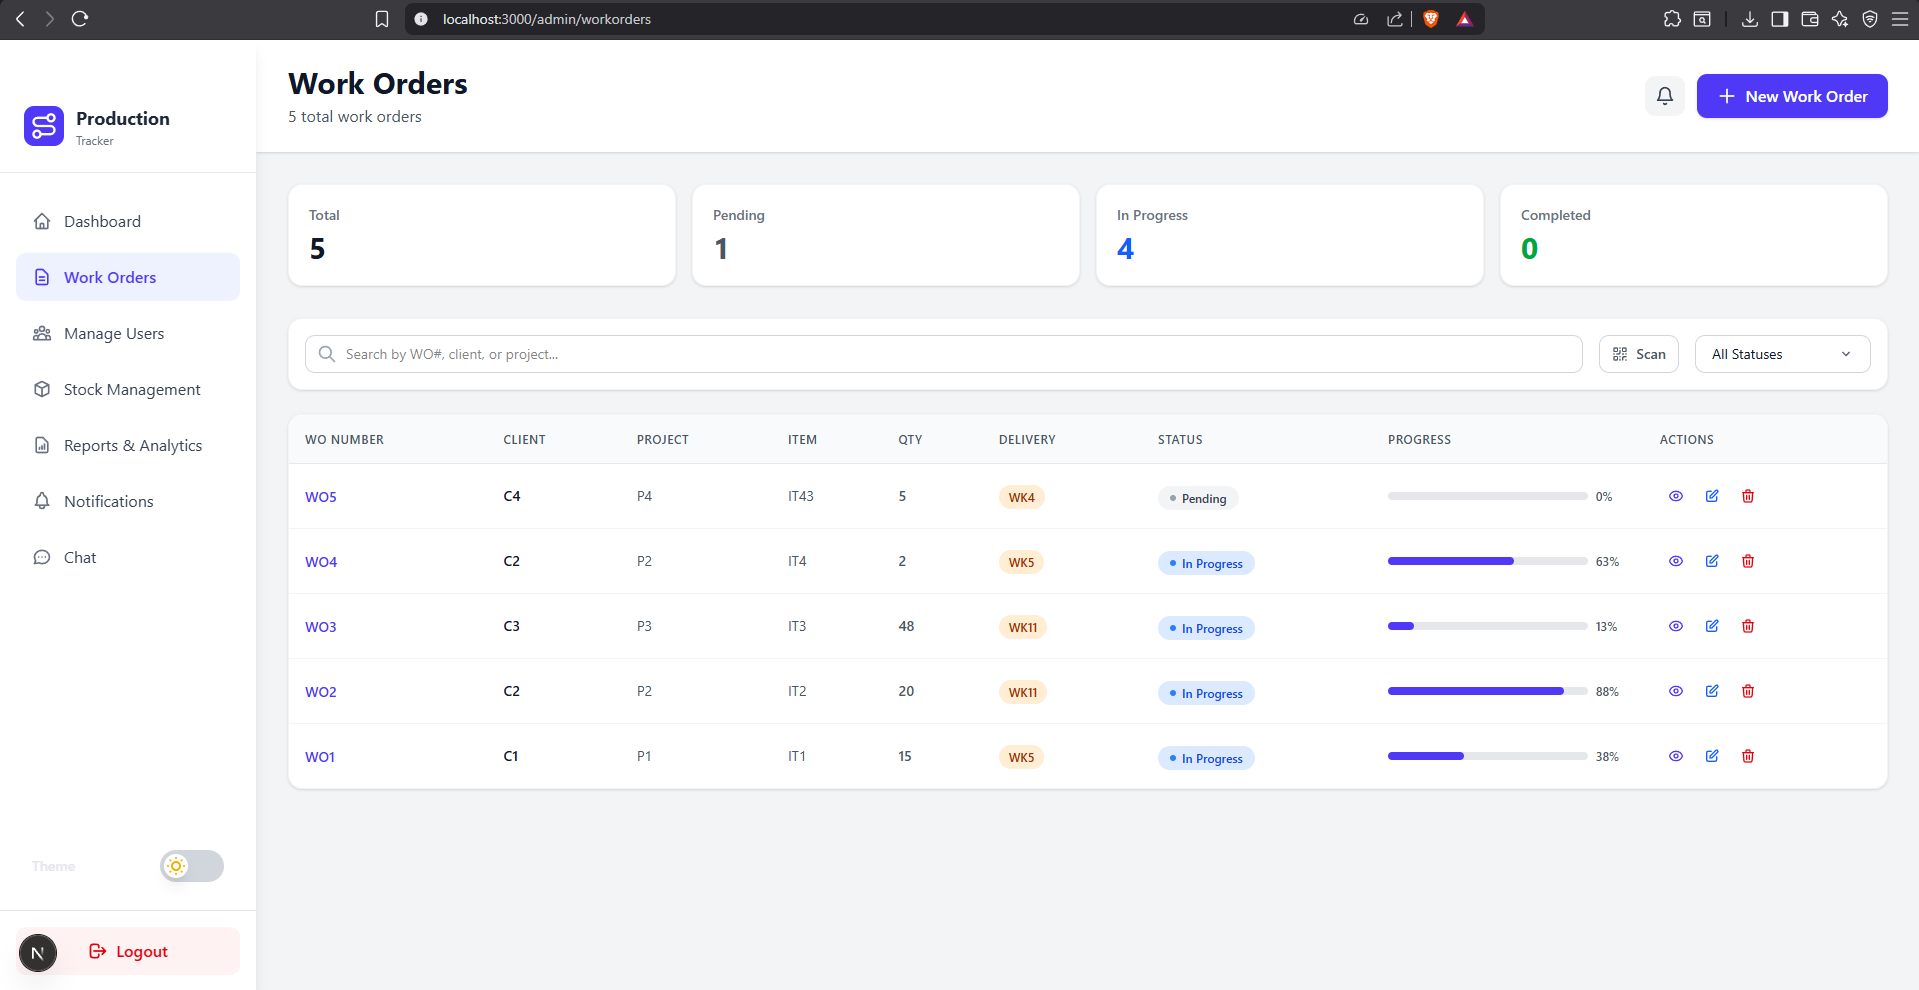
\includegraphics[width=\textwidth,keepaspectratio]{pictures/Workorder managment interface.png}
    \vspace*{\fill}
    \caption{Work Order Management Interface}
    \label{fig:work-order-management-interface}
\end{figure}
\begin{figure}[H]
    \centering

    \begin{minipage}[t]{0.48\textwidth}
        \centering
        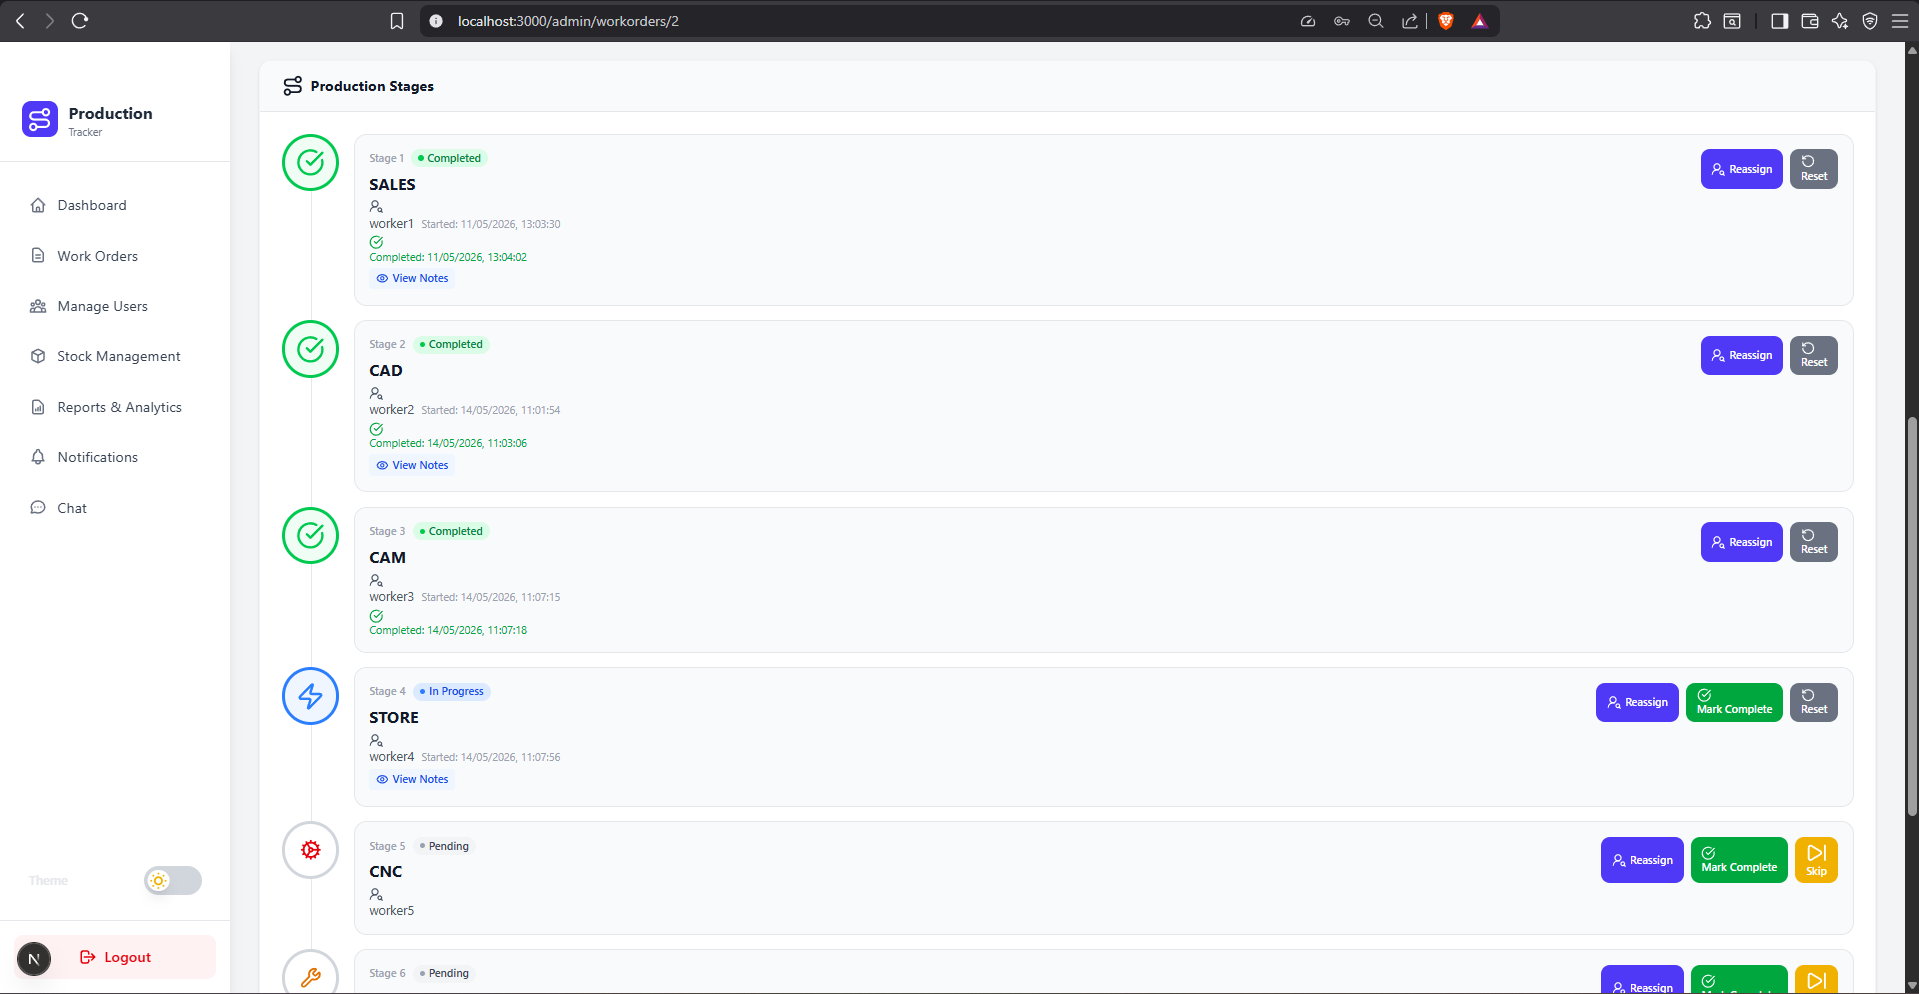
\includegraphics[width=\textwidth,keepaspectratio]{pictures/production stages admin view.png}
        \caption{Production Stages Admin View}
        \label{fig:production-stages-admin}
    \end{minipage}
    \hfill
    \begin{minipage}[t]{0.48\textwidth} 
        \centering
        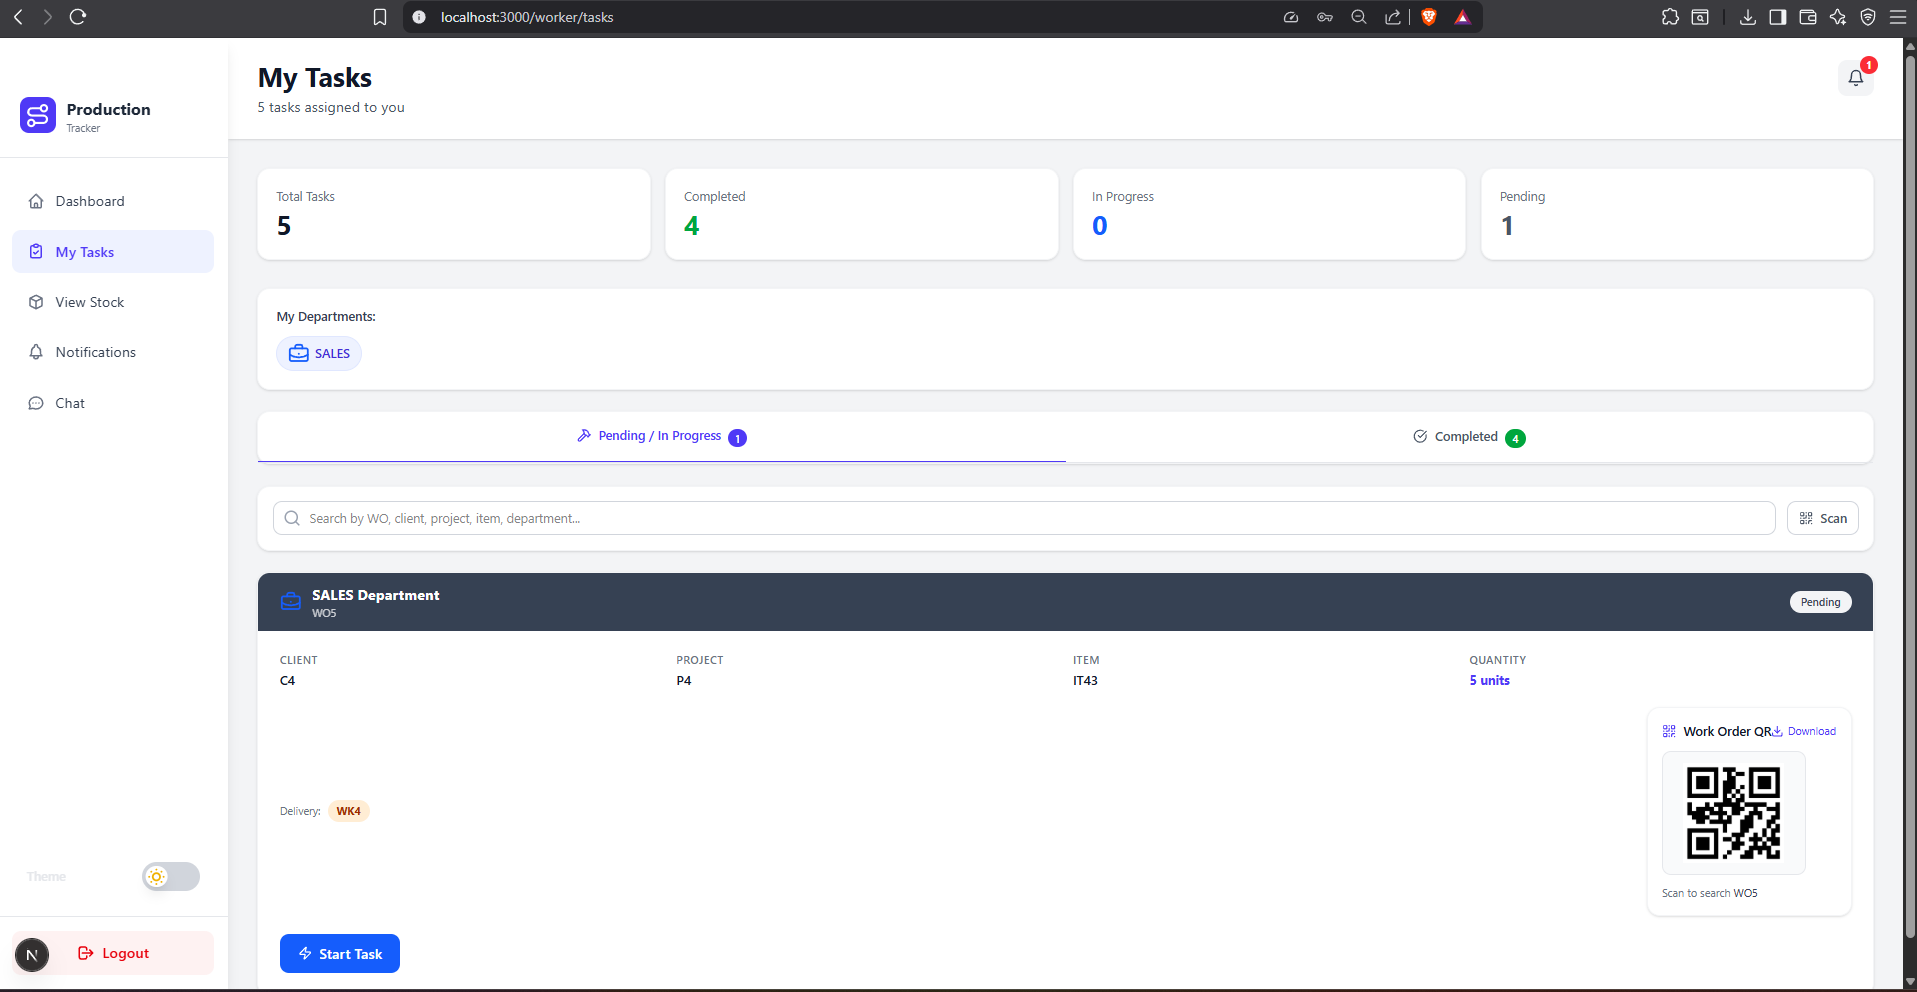
\includegraphics[width=\textwidth,keepaspectratio]{pictures/worker tasks view.png}
        \caption{Worker Tasks View}
        \label{fig:worker-tasks-view}
    \end{minipage}

\end{figure}
\section{Sprint 3: Stock Management}
\label{sec:sprint3}

\subsection{Sprint Backlog}
\label{sec:sprint3-backlog}
the table \ref{tab:sprint3-backlog} summarizes the user stories and tasks completed during Sprint 3.
\footnotesize
\begin{longtable}{|p{0.10\textwidth}|p{0.50\textwidth}|p{0.32\textwidth}|}
    \hline
    \textbf{ID} & \textbf{User Story} & \textbf{Tasks} \\
    \hline
    \endfirsthead
    \hline
    \textbf{ID} & \textbf{User Story} & \textbf{Tasks} \\
    \hline
    \endhead
    \hline
    \endfoot
    PB-08 & As an admin, I want to create, edit, and delete stock items so that inventory stays accurate. & Design inventory schema; \newline  Build stock registration UI; \newline  create Stock CRUD works \\
    \hline
    PB-09 & As a worker, I want to reserve stock items for my tasks and mark them as consumed when used. & create reservation logic; \newline  build reservation interface;  \\
    \hline
    PB-10 & As an administrator, I want to monitor stock reservations &  create reservation tracking functionality; \newline Build reservation tracking UI;\\
    \hline
    \caption{Sprint 3 Backlog}\label{tab:sprint3-backlog}\\
\end{longtable}
\normalsize

\subsection{Sprint 3 use case diagram}
the figure \ref{fig:sprint3-use-case-diagram} illustrates the main use cases implemented in Sprint 3, focusing on stock management features. It shows the interactions between administrators and workers with the system for managing stock items, reserving inventory, and monitoring reservations.
\begin{figure}[H]
    \centering
    
    \includegraphics[width=\textwidth,keepaspectratio]{pictures/sprint3 use case diagram.drawio.png}
    \vspace*{\fill}
    \caption{Sprint 3 Use Case Diagram}
    \label{fig:sprint3-use-case-diagram}
\end{figure}


\subsection{Sprint 3: Application Interface Overview}
\label{sec:sprint3-interfaces}
the figures \ref{fig:inventory-admin-view} and \ref{fig:inventory-reservations-admin-view} show the inventory management interfaces for administrators, allowing them to manage stock items and monitor reservations. 
\begin{figure}[H]
    \centering

    \begin{minipage}[t]{0.48\textwidth}
        \centering
        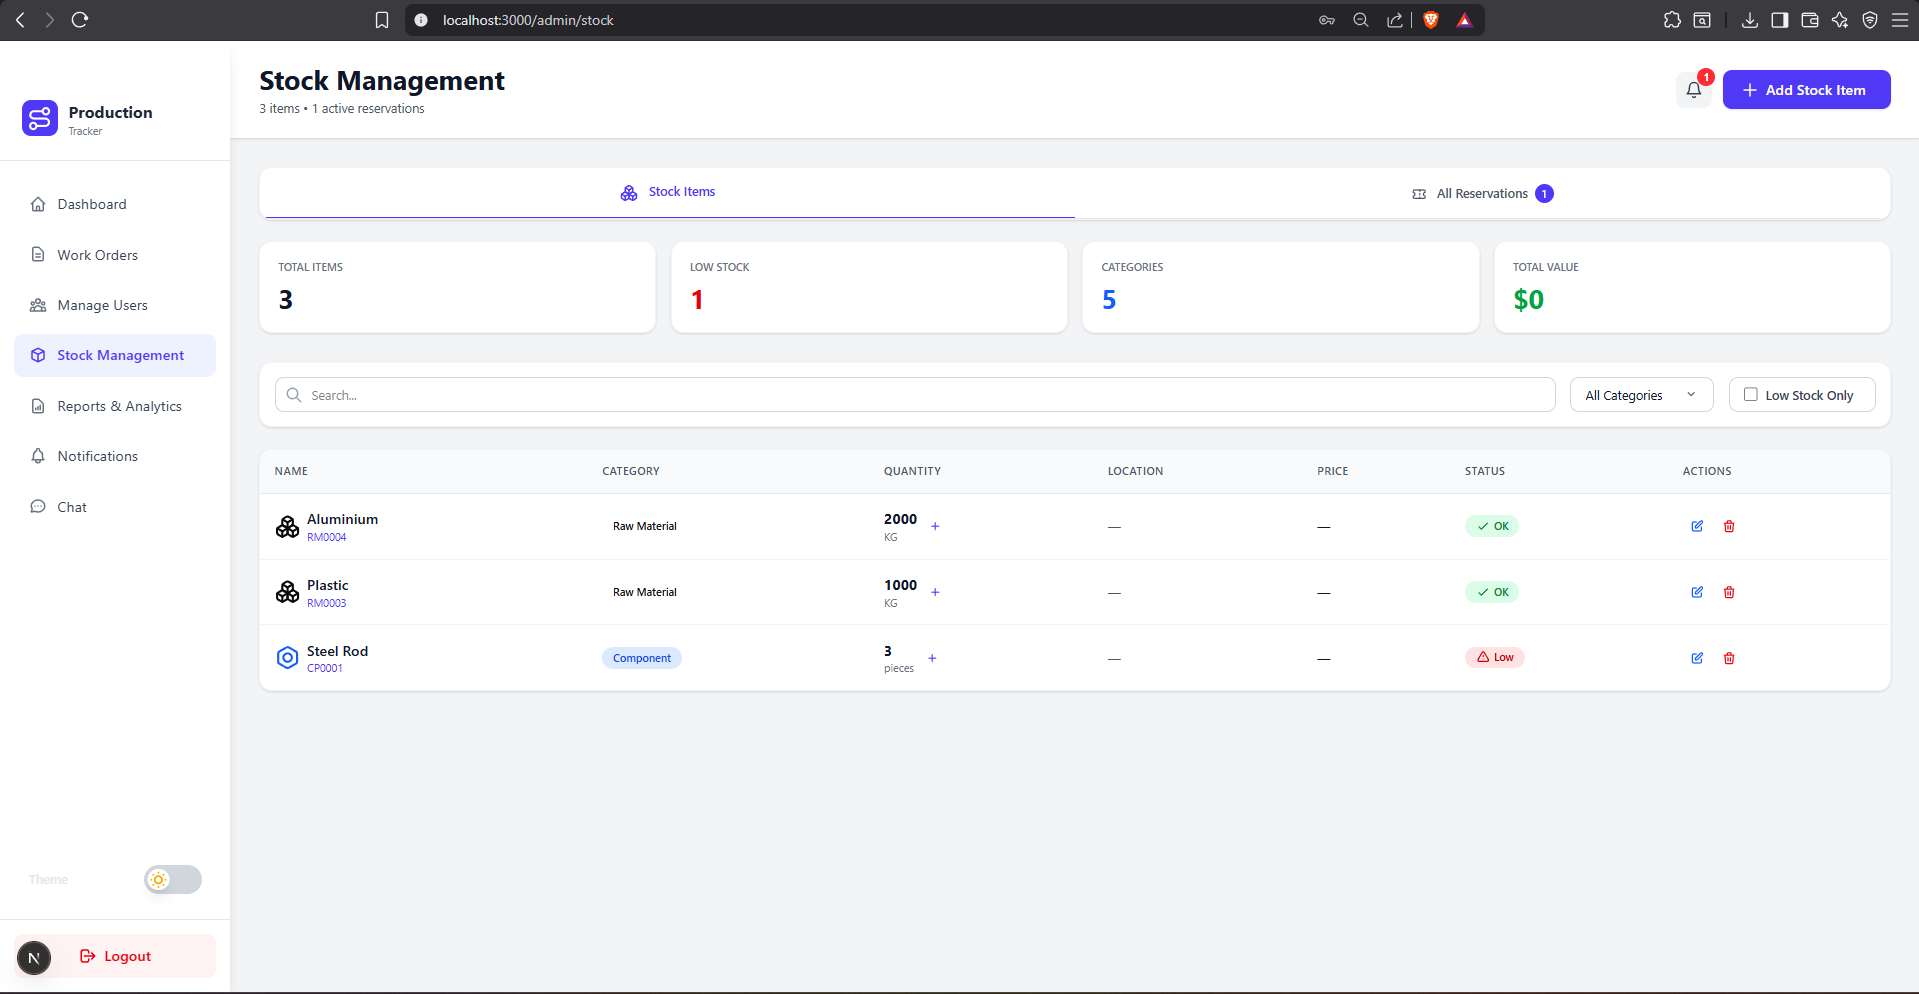
\includegraphics[width=\textwidth,keepaspectratio]{pictures/inventory admin view.png}
        \caption{Inventory Admin View}
        \label{fig:inventory-admin-view}
    \end{minipage}
    \hfill
    \begin{minipage}[t]{0.48\textwidth} 
        \centering
        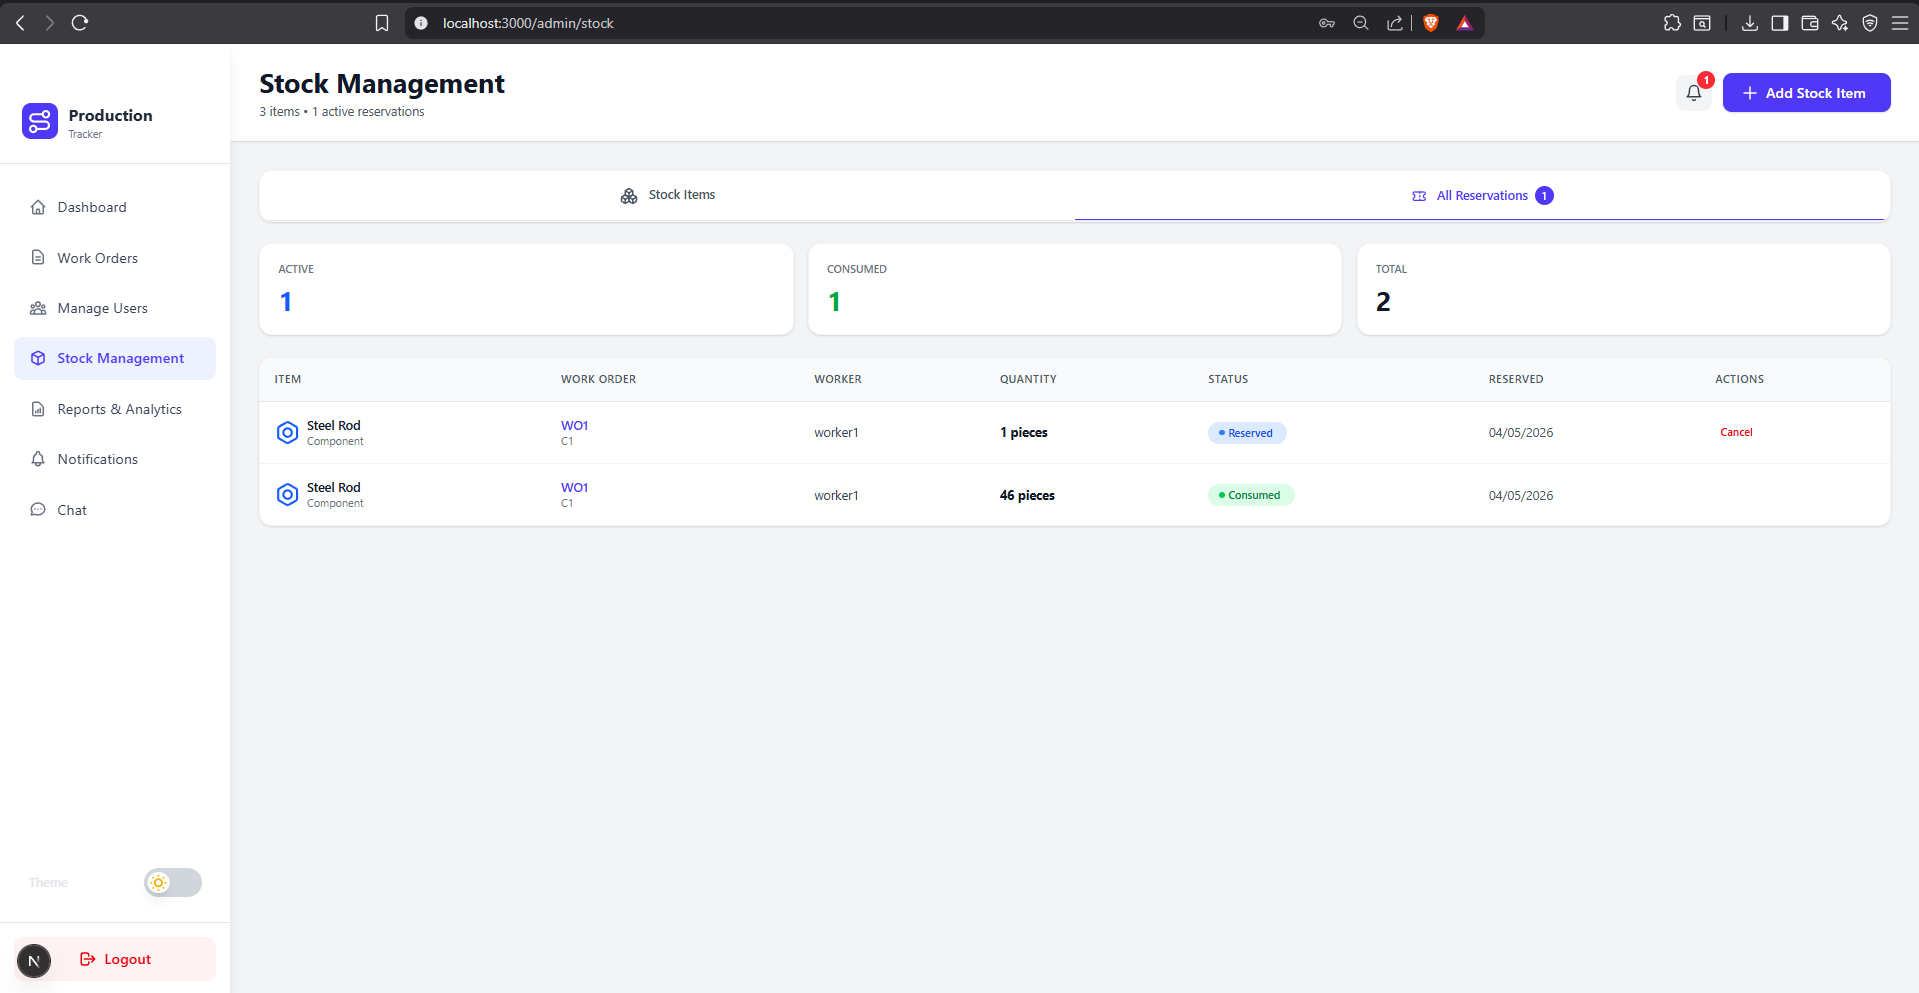
\includegraphics[width=\textwidth,keepaspectratio]{pictures/inventory reservations admin view.png}
        \caption{Inventory Reservations Admin View}
        \label{fig:inventory-reservations-admin-view}
    \end{minipage}

\end{figure}
 The figures \ref{fig:inventory-worker-view} and \ref{fig:inventory-reservations-worker-view} show the inventory interfaces for workers, enabling them to view available stock and manage their reservations effectively.
\begin{figure}[H]
    \centering

    \begin{minipage}[t]{0.48\textwidth}
        \centering
        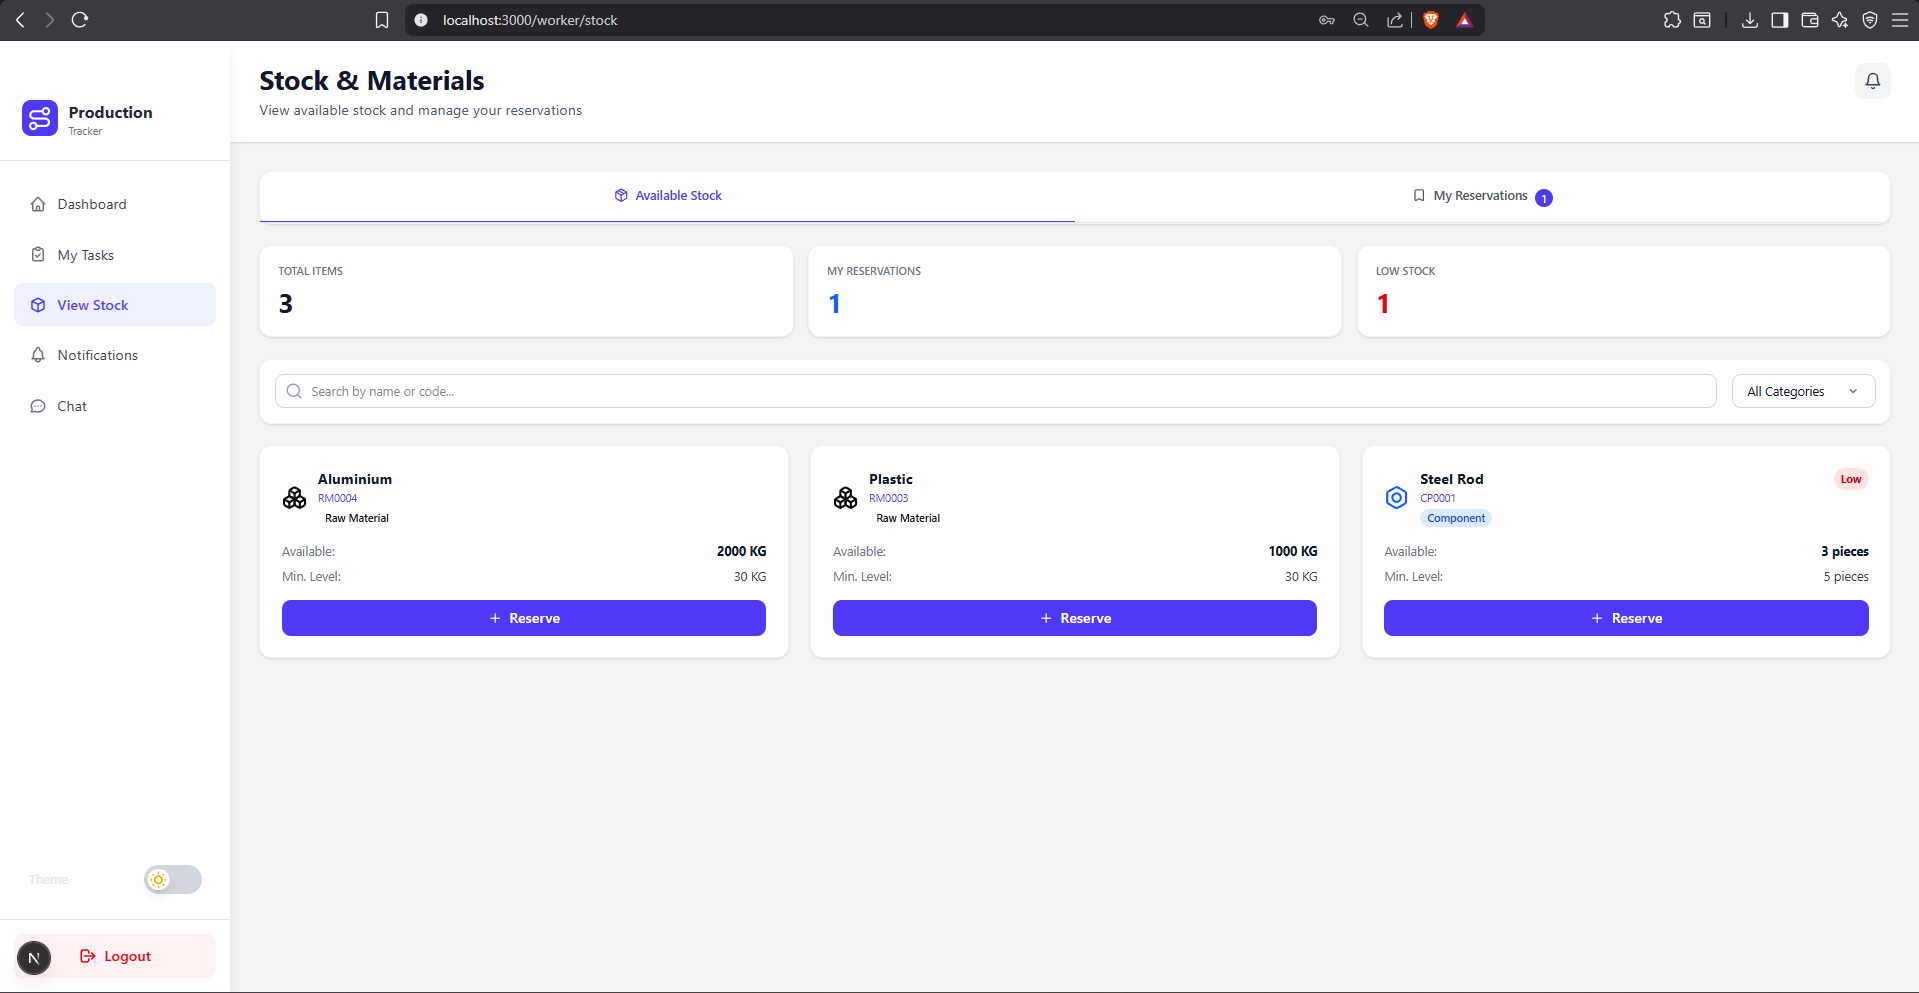
\includegraphics[width=\textwidth,keepaspectratio]{pictures/inventory worker view.png}
        \caption{Inventory Worker View}
        \label{fig:inventory-worker-view}
    \end{minipage}
    \hfill
    \begin{minipage}[t]{0.48\textwidth} 
        \centering
        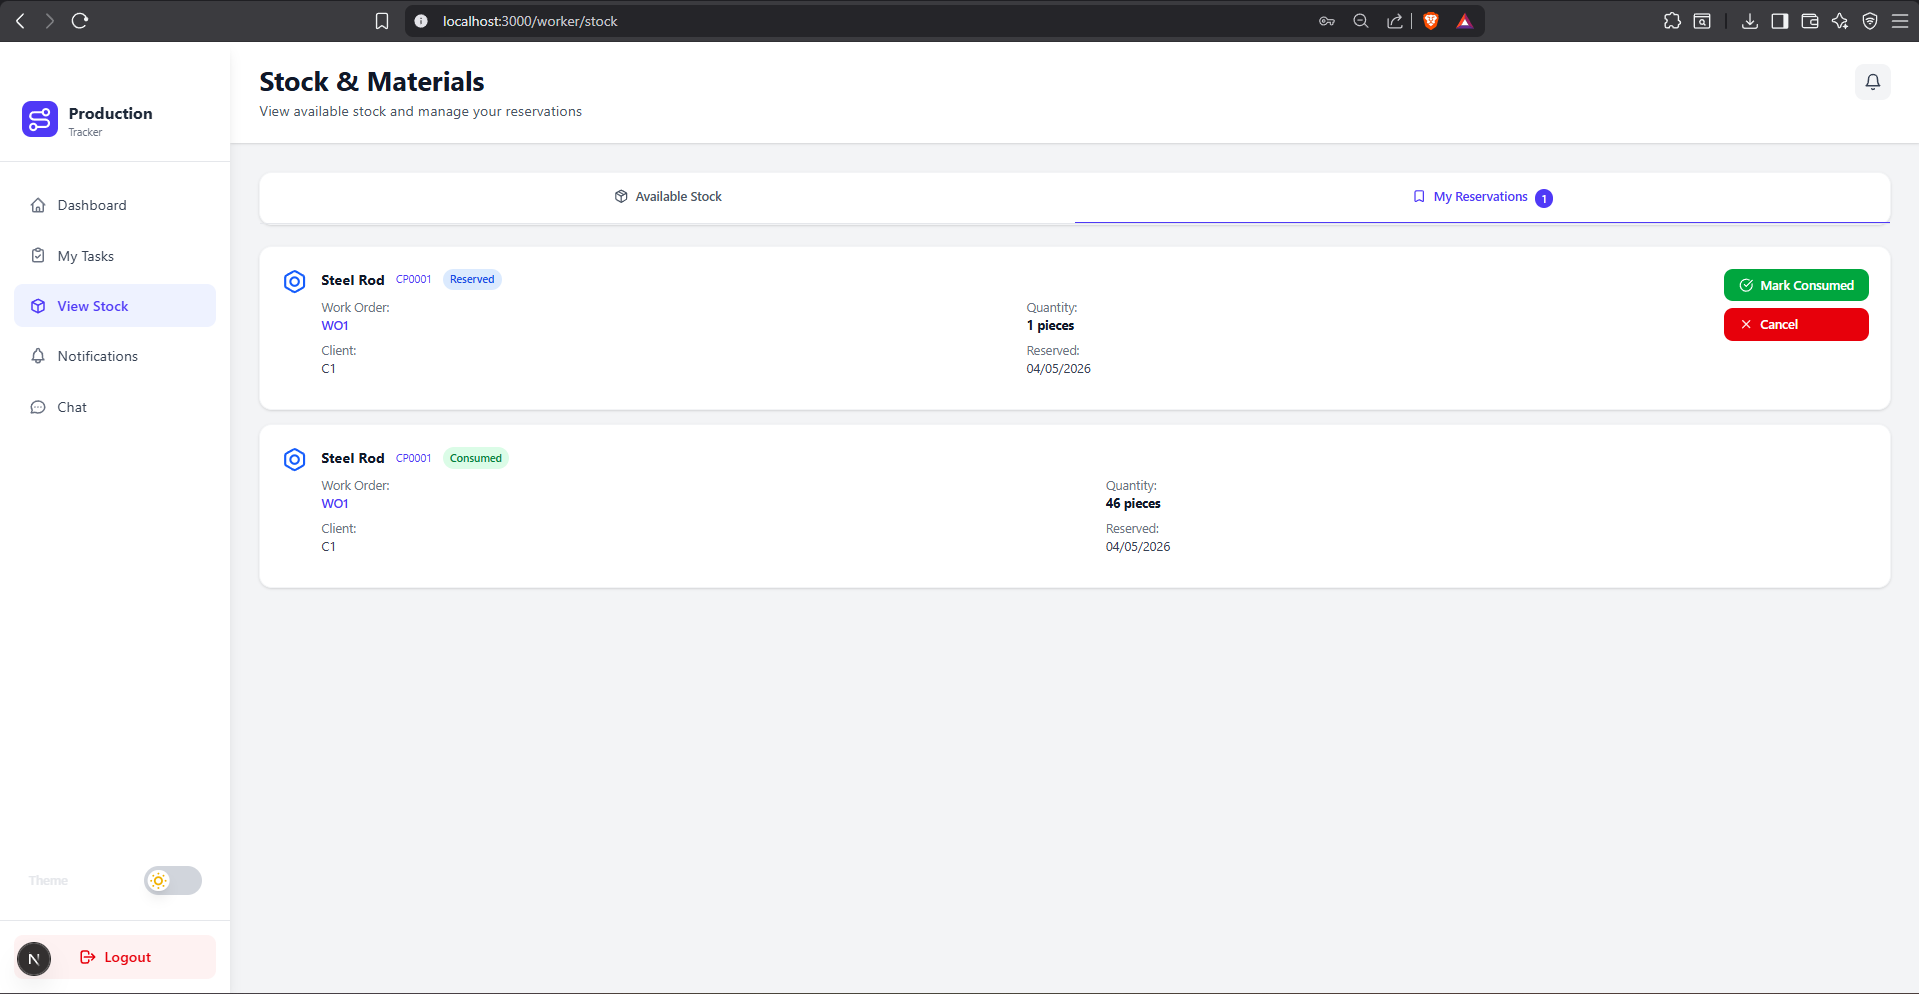
\includegraphics[width=\textwidth,keepaspectratio]{pictures/inventory reservations worker view.png}
        \caption{Inventory Reservations Worker View}
        \label{fig:inventory-reservations-worker-view}
    \end{minipage}

\end{figure}
\section{Conclusion}
\label{sec:release1-conclusion}

The first release completed the core features that formed the foundation of the Production Tracker software, by providing security through the implementation of authentication processes, building the core functionality that formed the production flow process, and finally, implementing inventory management. These three sprints lasted 21 days each, giving a total of 63 days, after which the second release will be covered in the next chapter.


% Chapter 4: Implementation
\chapter{Release 2}
\label{chap:release2}

\section{Introduction}
\label{sec:release2-intro}

Release 2 encompasses the final two sprints of the Production Tracker project, focusing on real-time communication through integrated chat systems, quick identification with QR code technology, intelligent reporting with AI assistance, and comprehensive notification management. This release delivers advanced features that enhance user collaboration, operational visibility, and decision-making capabilities.

\section{Sprint 4: Notes, Real-Time Chat, and Notifications}
\label{sec:sprint4}

\subsection{Sprint Backlog}
\label{sec:sprint4-backlog}
the table \ref{tab:sprint4-backlog} summarizes the user stories and tasks completed during Sprint 4:
\footnotesize
\begin{longtable}{|p{0.10\textwidth}|p{0.50\textwidth}|p{0.32\textwidth}|}
    \caption{Sprint 4 Backlog}\label{tab:sprint4-backlog}\\
    \hline
    \textbf{ID} & \textbf{User Story} & \textbf{Tasks} \\
    \hline
    \endfirsthead
    \hline
    \textbf{ID} & \textbf{User Story} & \textbf{Tasks} \\
    \hline
    \endhead
    \hline
    \endfoot
    PB-11 & As a worker, I want to add notes on work stages so that operational details are documented. & Create notes logic; \newline  Build notes UI; \newline  Add note timestamp and author tracking \\
    \hline
    PB-12 & As a user, I want to chat with other users in real time so that I can discuss issues. & Setup real-time communication; \newline  Build chat interface; \newline  Implement message history \\
    \hline
    PB-13 & As a user, I want to attach files in chat so that I can share documents and evidence. & Build file upload handler; \newline   Add file attachment UI \\
    \hline
    PB-14 & As a user, I want to receive notifications so that I do not miss important events. & Implement notification service; \newline  Build notification UI; \newline  Add notification management \\
    \hline
\end{longtable}
\normalsize

\subsection{Sprint 4 Use Case Diagram}
the figure \ref{fig:sprint4-use-case-diagram} illustrates the main use cases implemented in Sprint 4, focusing on real-time communication and notification features. It shows the interactions between users for adding notes, engaging in chat conversations, attaching files, and managing notifications within the system.
\begin{figure}[H]
    \centering
    
    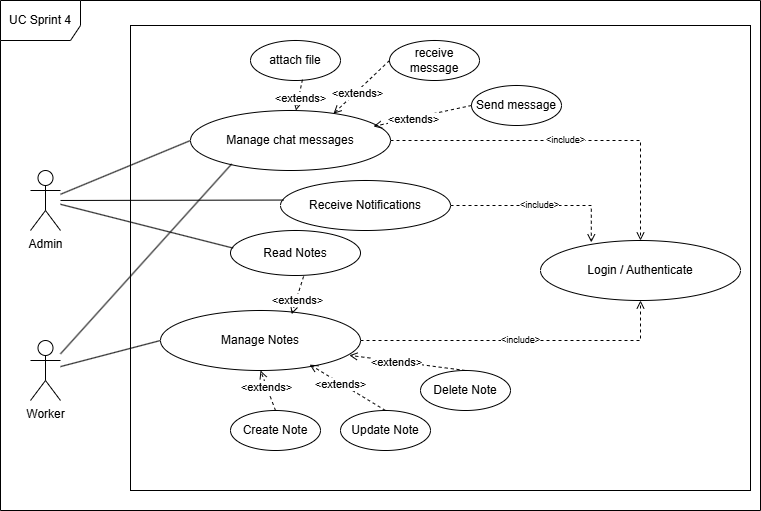
\includegraphics[width=\textwidth,keepaspectratio]{pictures/Sprint 4 UC Diagram.drawio.png}
    \vspace*{\fill}
    \caption{Sprint 4 Use Case Diagram}
    \label{fig:sprint4-use-case-diagram}
\end{figure}
\vspace{1cm}
\subsection{Sequence Diagram for Real-Time Messaging}
the figure \ref{fig:real-time-chat-sequence-diagram} illustrates the sequence of interactions that occur during a real-time chat session between two users. It shows how messages are sent, received, and persisted in the system, highlighting the use of Socket.IO for real-time communication and the integration with the database for message storage.
\begin{sidewaysfigure}
    \centering
    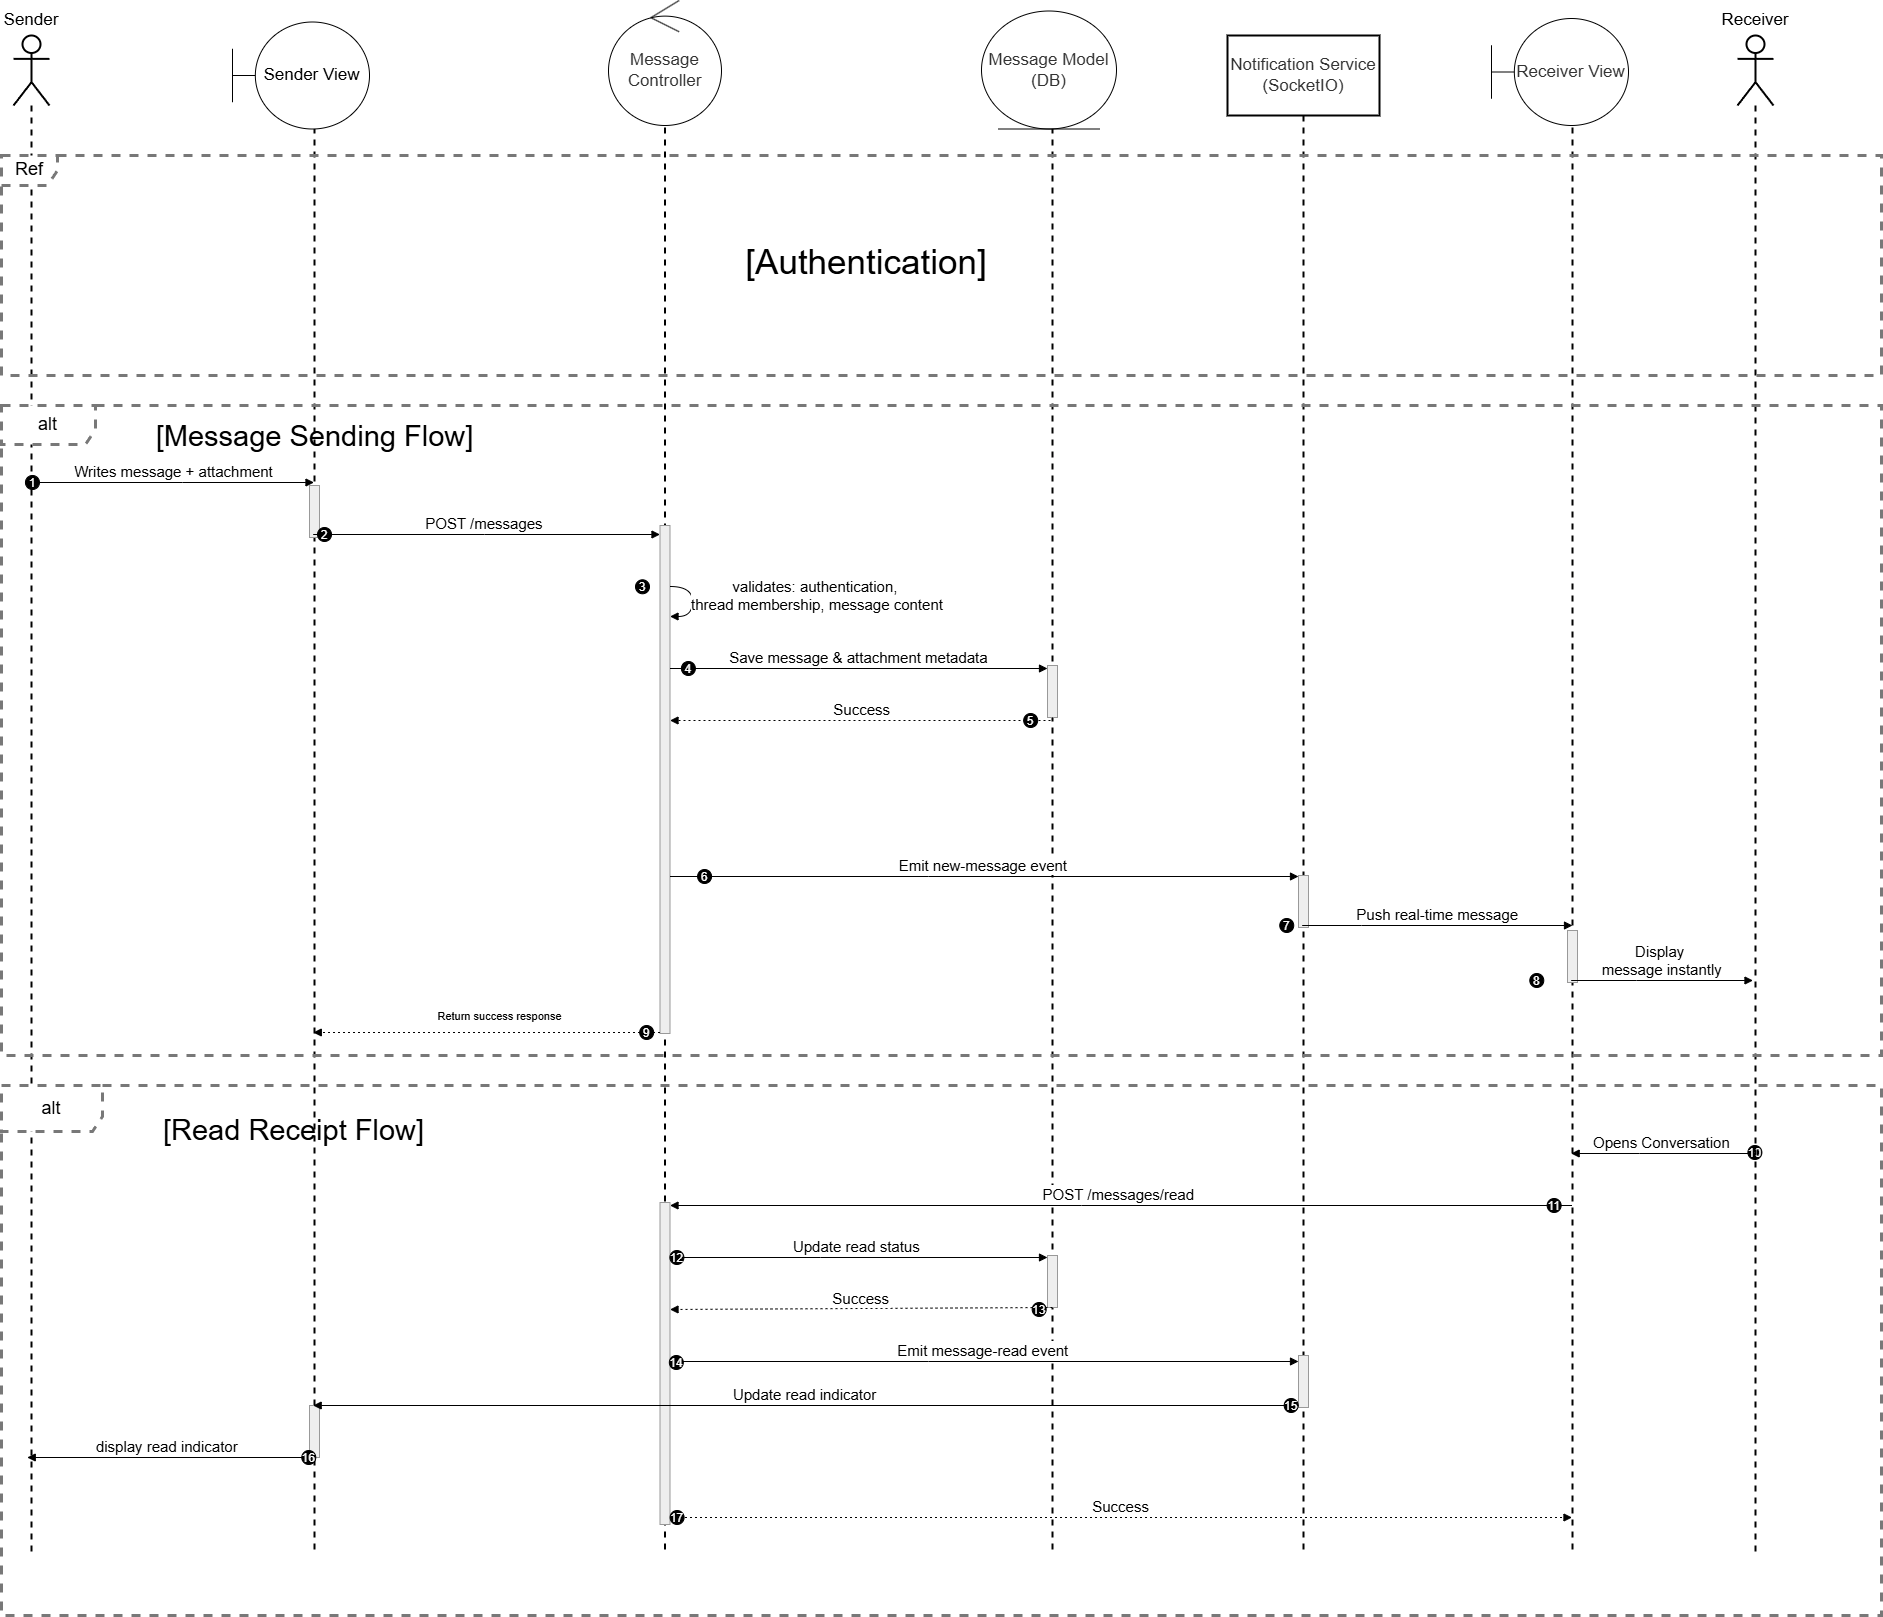
\includegraphics[width=0.8\textheight]{pictures/Real-time chat message flow.drawio.png}
    \caption{Real-Time Chat Message Flow Sequence Diagram}
    \label{fig:real-time-chat-sequence-diagram}
\end{sidewaysfigure}
\vspace{1cm}
\subsection{Sprint 4: Application Interface Overview}

\label{sec:sprint4-interfaces}
the figures \ref{fig:note-management-worker}, \ref{fig:notes-history-admin} illustrate the note management interfaces for workers and administrators, respectively. The worker view allows users to add and view notes related to their tasks, while the admin view provides a comprehensive history of all notes for monitoring and analysis.
\begin{figure}[H]
    \centering

    \begin{minipage}[t]{0.48\textwidth}
        \centering
        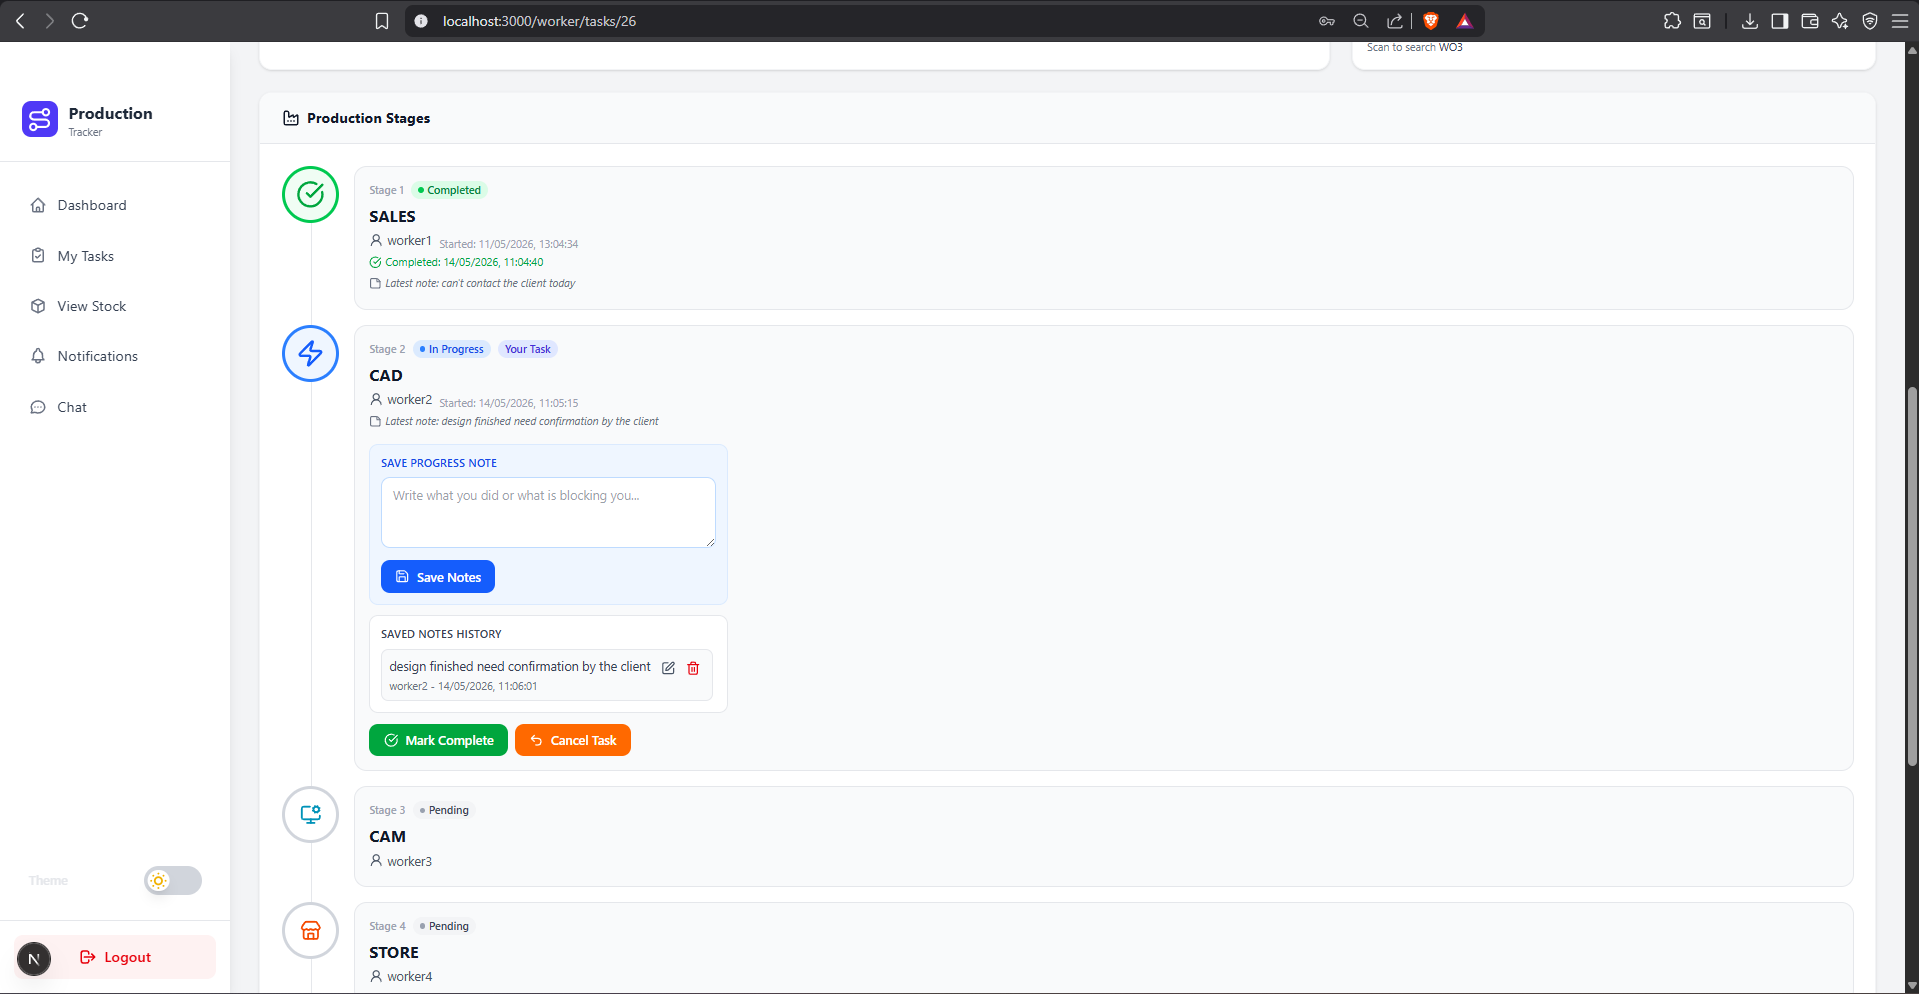
\includegraphics[width=\textwidth,keepaspectratio]{pictures/note managment worker view.png}
        \caption{Note Management Worker View}
        \label{fig:note-management-worker}
    \end{minipage}
    \hfill
    \begin{minipage}[t]{0.48\textwidth} 
        \centering
        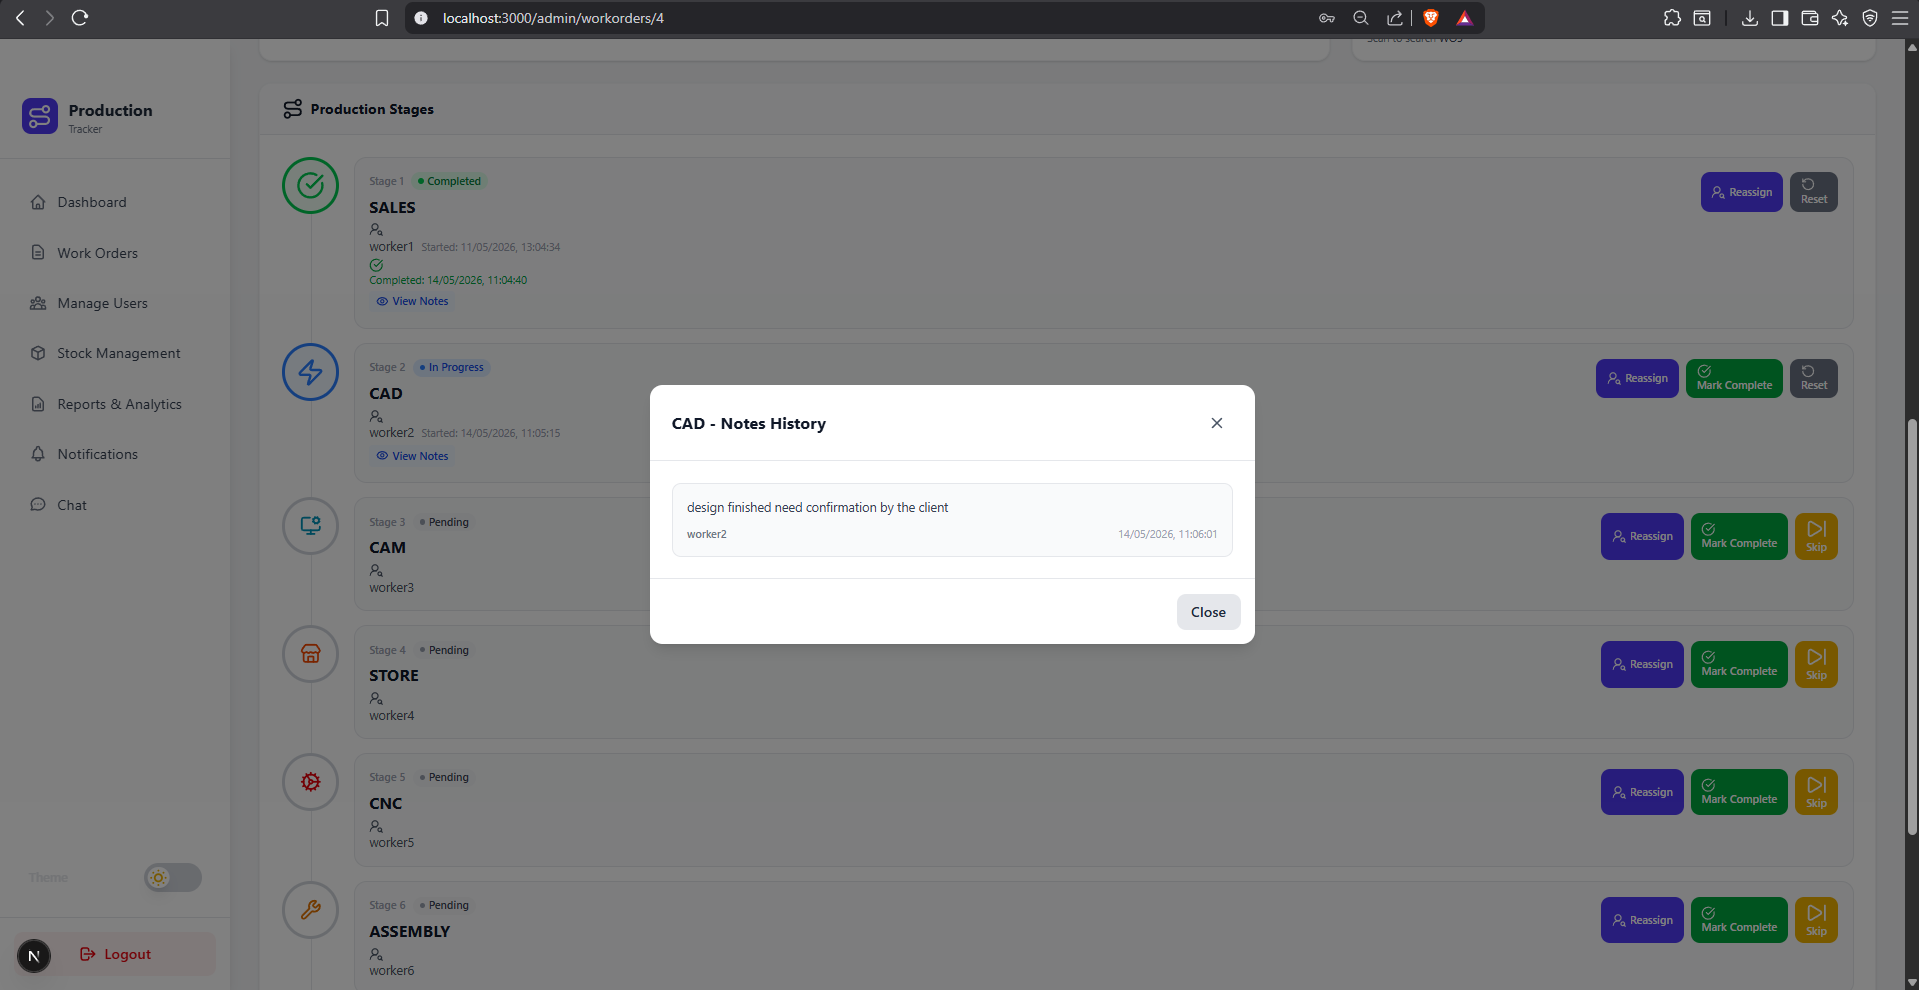
\includegraphics[width=\textwidth,keepaspectratio]{pictures/notes history admin view.png}
        \caption{Notes History Admin View}
        \label{fig:notes-history-admin}
    \end{minipage}

\end{figure}

the figures \ref{fig:chat-messaging-worker} and \ref{fig:chat-messaging-admin} provide an overview of the real-time chat messaging interfaces.
\begin{figure}[H]
    \centering

    \begin{minipage}[t]{0.48\textwidth}
        \centering
        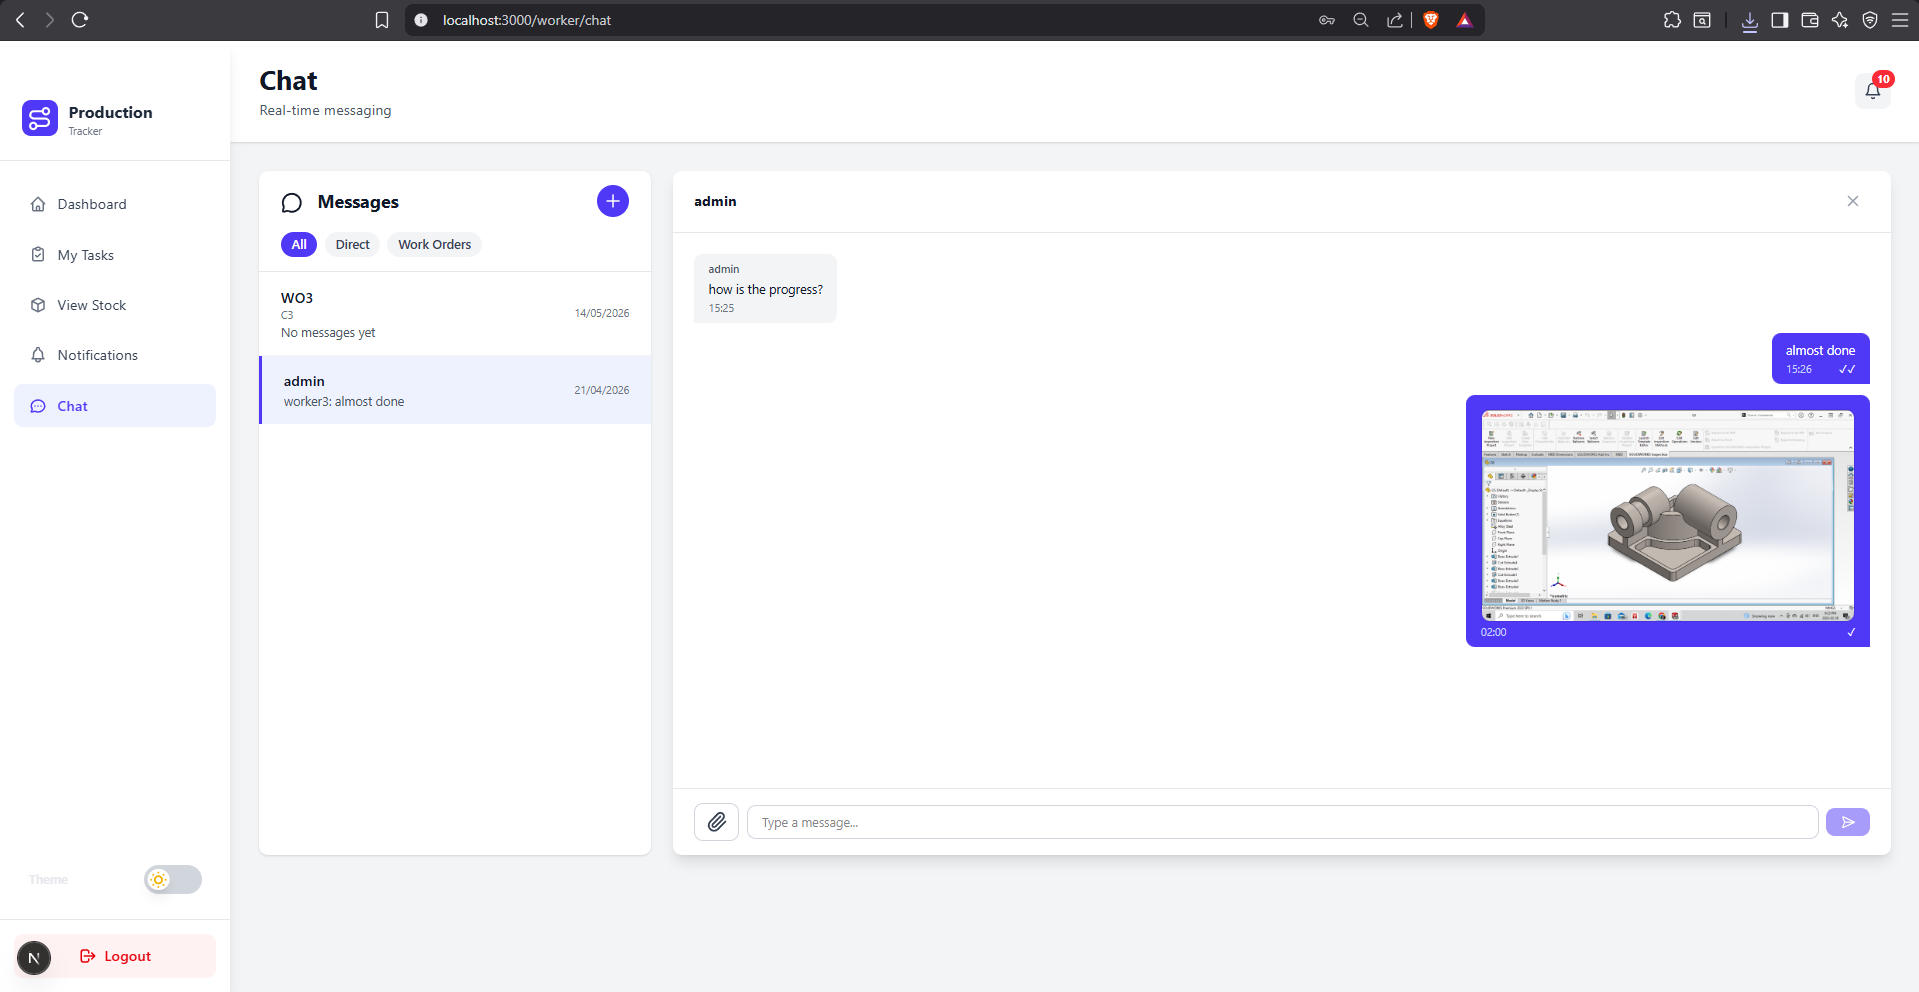
\includegraphics[width=\textwidth,keepaspectratio]{pictures/chat messaging interface worker view.png}
        \caption{Chat Messaging Interface Worker View}
        \label{fig:chat-messaging-worker}
    \end{minipage}
    \hfill
    \begin{minipage}[t]{0.48\textwidth} 
        \centering
        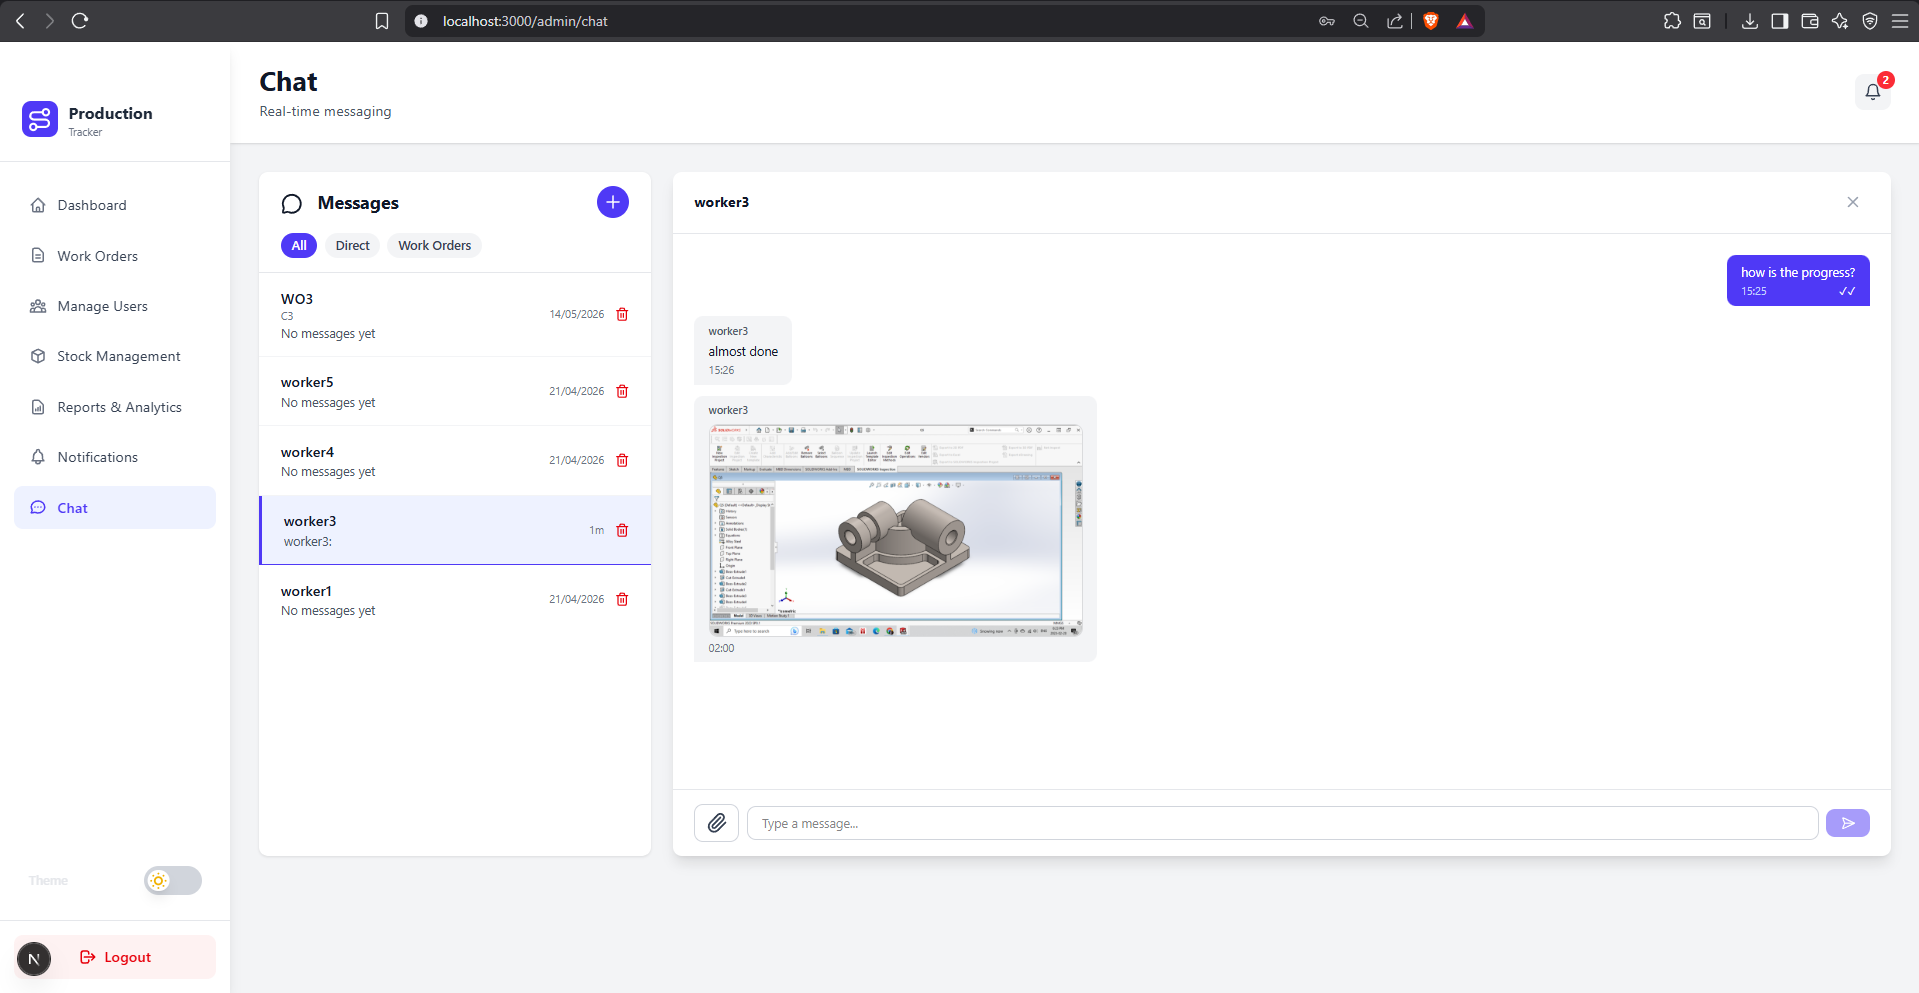
\includegraphics[width=\textwidth,keepaspectratio]{pictures/chat messaging admin view.png}
        \caption{Chat Messaging Interface Admin View}
        \label{fig:chat-messaging-admin}
    \end{minipage}

\end{figure}
the figure \ref{fig:notification-center} illustrates the notification center interface for managing alerts and notifications within the system.
\begin{figure}[H]
    \centering
\begin{minipage}[t]{0.48\textwidth} 
        \centering
        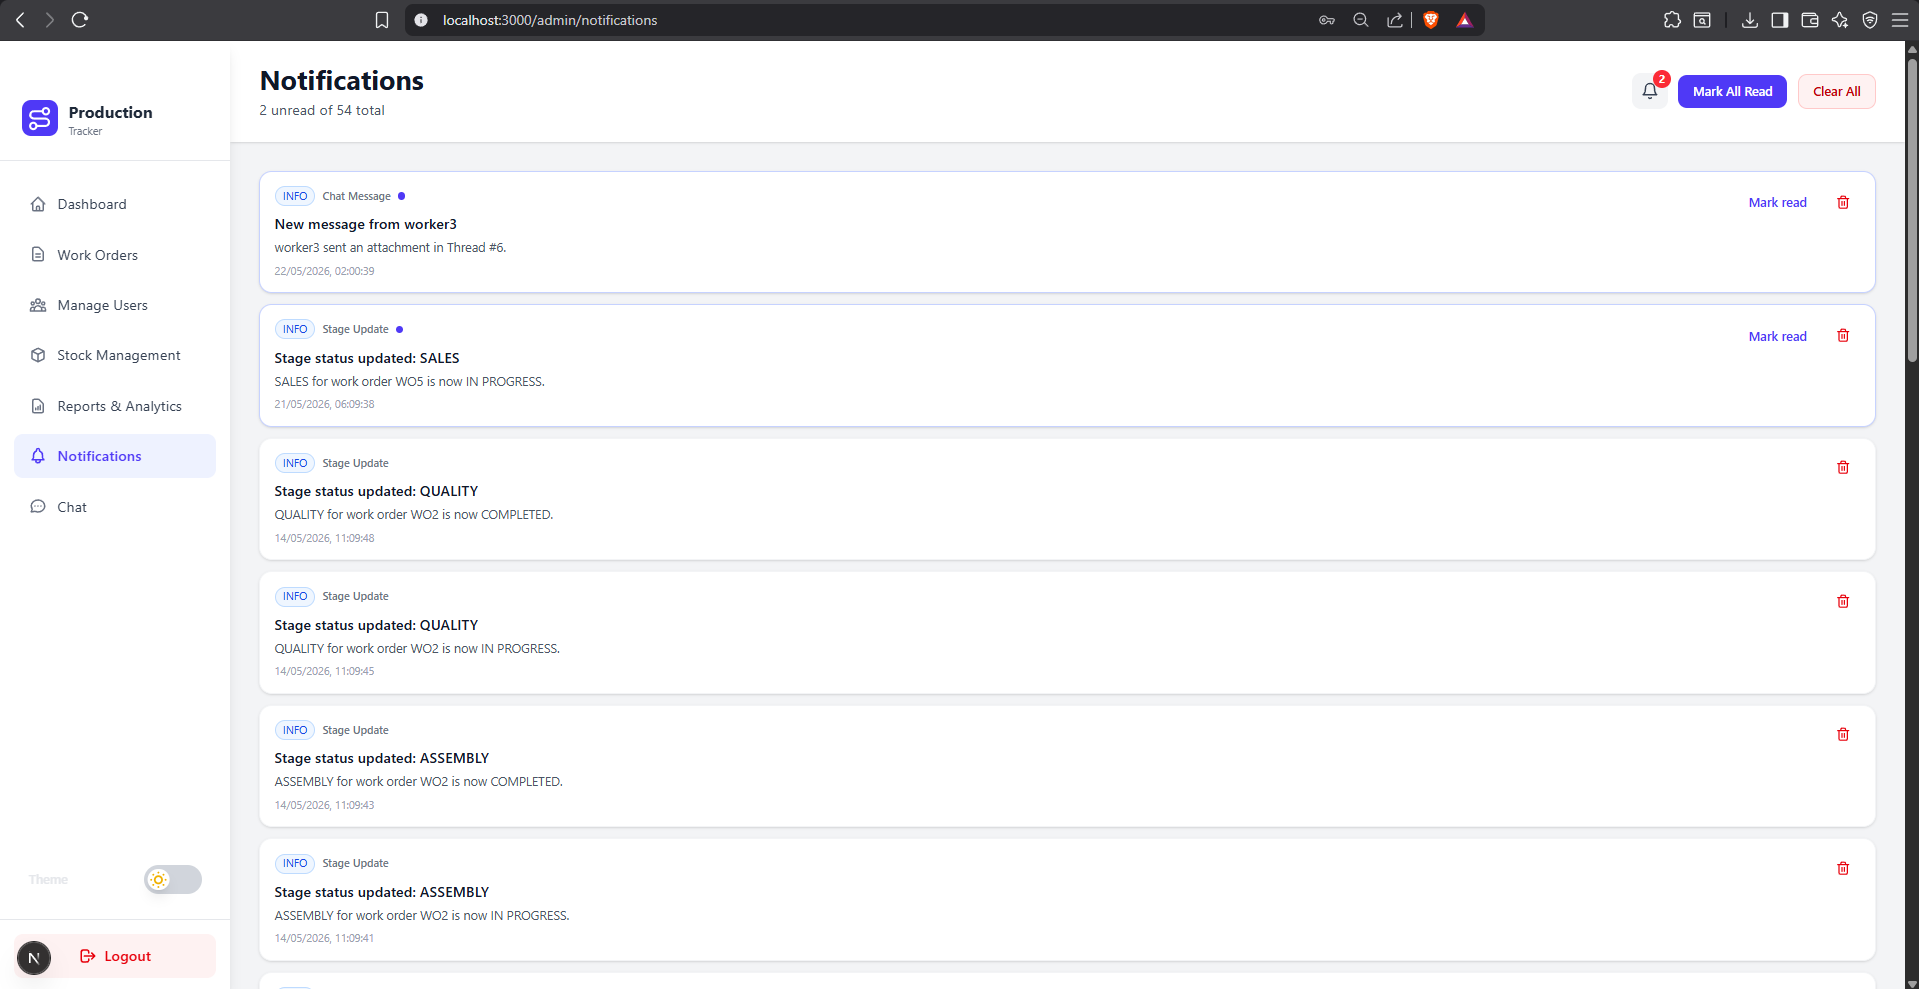
\includegraphics[width=\textwidth,keepaspectratio]{pictures/notification center.png}
        \caption{Notification Center}
        \label{fig:notification-center}
    \end{minipage}
\end{figure}
\section{Sprint 5: QR Codes, Analytics, and AI Reporting}
\label{sec:sprint5}

\subsection{Sprint Backlog}
\label{sec:sprint5-backlog}
the table \ref{tab:sprint5-backlog} summarizes the user stories and tasks completed during Sprint 5:

\footnotesize
\begin{longtable}{|p{0.10\textwidth}|p{0.50\textwidth}|p{0.32\textwidth}|}
    \caption{Sprint 5 Backlog}\label{tab:sprint5-backlog}\\
    \hline
    \textbf{ID} & \textbf{User Story} & \textbf{Tasks} \\
    \hline
    \endfirsthead
    \hline
    \textbf{ID} & \textbf{User Story} & \textbf{Tasks} \\
    \hline
    \endhead
    \hline
    \endfoot
    PB-15 & As an administrator, I want generated QR codes for work orders so that identification is faster. & Implement QR code library; \newline  Build generation API; \newline  Add QR display  \\
    \hline
    PB-16 & As a user, I want to scan QR codes so that I can quickly search and access work orders . & Integrate QR scanner; \newline  Build scan interface; \newline  Add scan result handler \\
    \hline
    PB-17 & As an administrator, I want AI-assisted reporting so that I can make faster decisions. & Setup reporting engine; \newline  Integrate AI analysis; \newline  Build dashboard UI \\
    \hline
    PB-18 & As an administrator, I want a analytical dashboard for the production data. & Build analytics UI; \newline  Integrate data visualization; \\
    \hline
\end{longtable}
\normalsize

\subsection{Sprint 5 Use Case Diagram}
\label{sec:sprint5-use-case-diagram}
the figure \ref{fig:sprint5-use-case-diagram} illustrates the main use cases implemented in Sprint 5:
\begin{figure}[H]
    \centering
    
    \includegraphics[width=0.8\textwidth,
    height=0.6\textheight,
    keepaspectratio]{pictures/Sprint 5 UC Diagram.drawio.png}
    \vspace*{\fill}
    \caption{Sprint 5 Use Case Diagram}
    \label{fig:sprint5-use-case-diagram}
\end{figure}

\subsection{Sequence Diagram for AI-Based Report Generation}
\label{sec:sprint5-sequence-diagram}
the figure \ref{fig:sprint5-sequence-diagram} illustrates the sequence of interactions that occur during the AI-based report generation process. It shows how data is collected, processed, and analyzed using AI to generate insightful reports for administrators.
\begin{figure}[H]
    \centering
    
    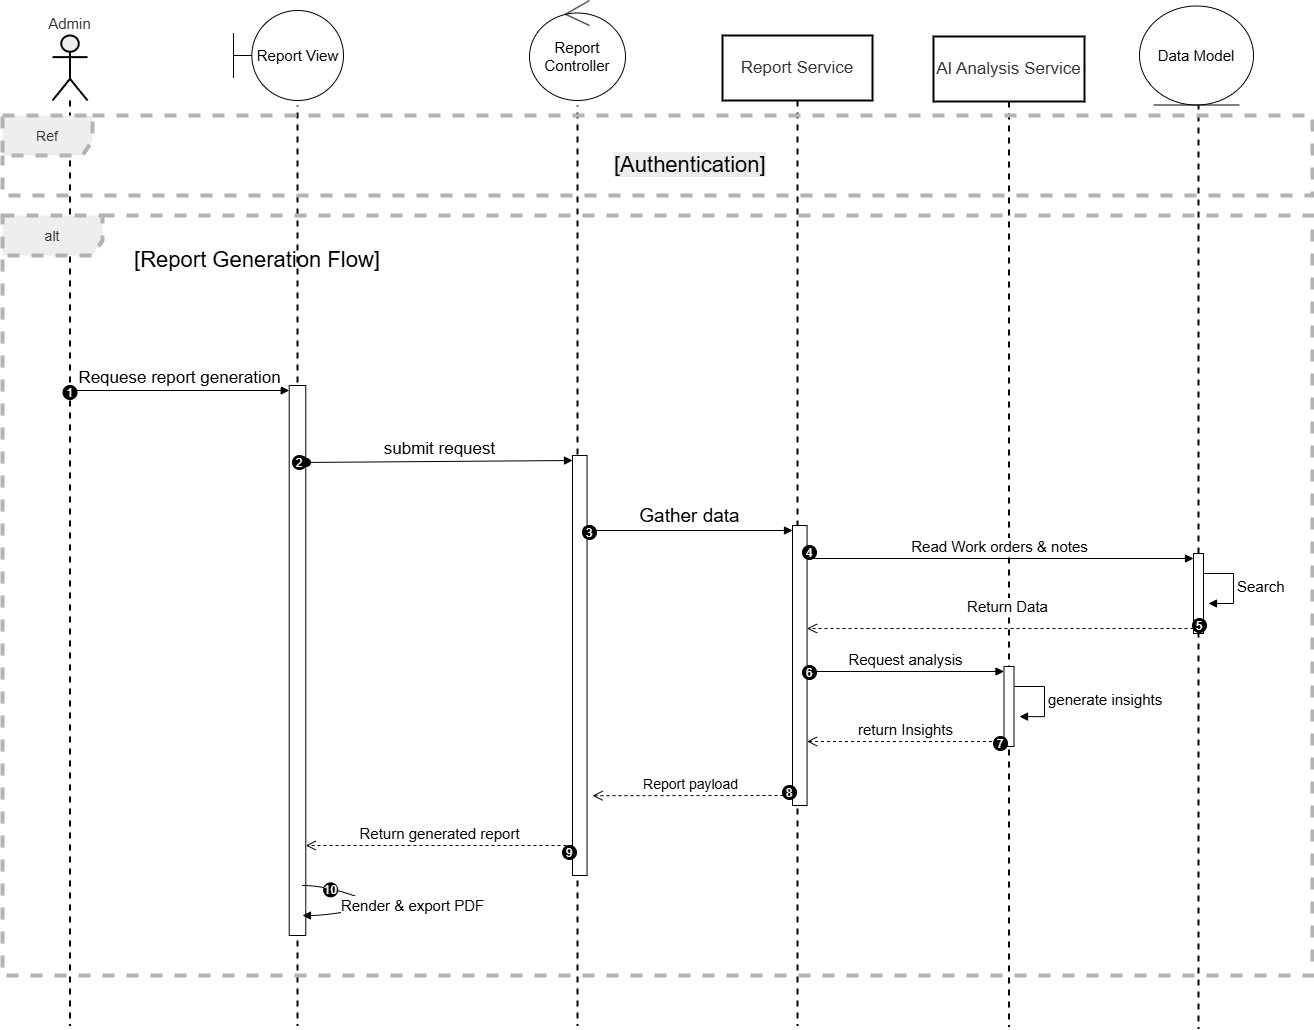
\includegraphics[width=\textwidth,
    height=0.6\textheight,
    keepaspectratio]{pictures/AI report sequence diagram.drawio.png}
    \vspace*{\fill}
    \caption{Sequence Diagram for AI-Based Report Generation}
    \label{fig:sprint5-sequence-diagram}
\end{figure}

\subsection{Sprint 5: Application Interface Overview}
the figures \ref{fig:workorder-details-with-qr} and \ref{fig:qr-code-scanner} illustrate the interfaces for work order details with QR code display and the QR code scanner, respectively. The work order details interface allows users to view comprehensive information about a work order along with a generated QR code for quick access, while the QR code scanner interface enables users to scan codes and retrieve associated work order information efficiently.
\begin{figure}[H]
    \centering

    \begin{minipage}[t]{0.48\textwidth}
        \centering
        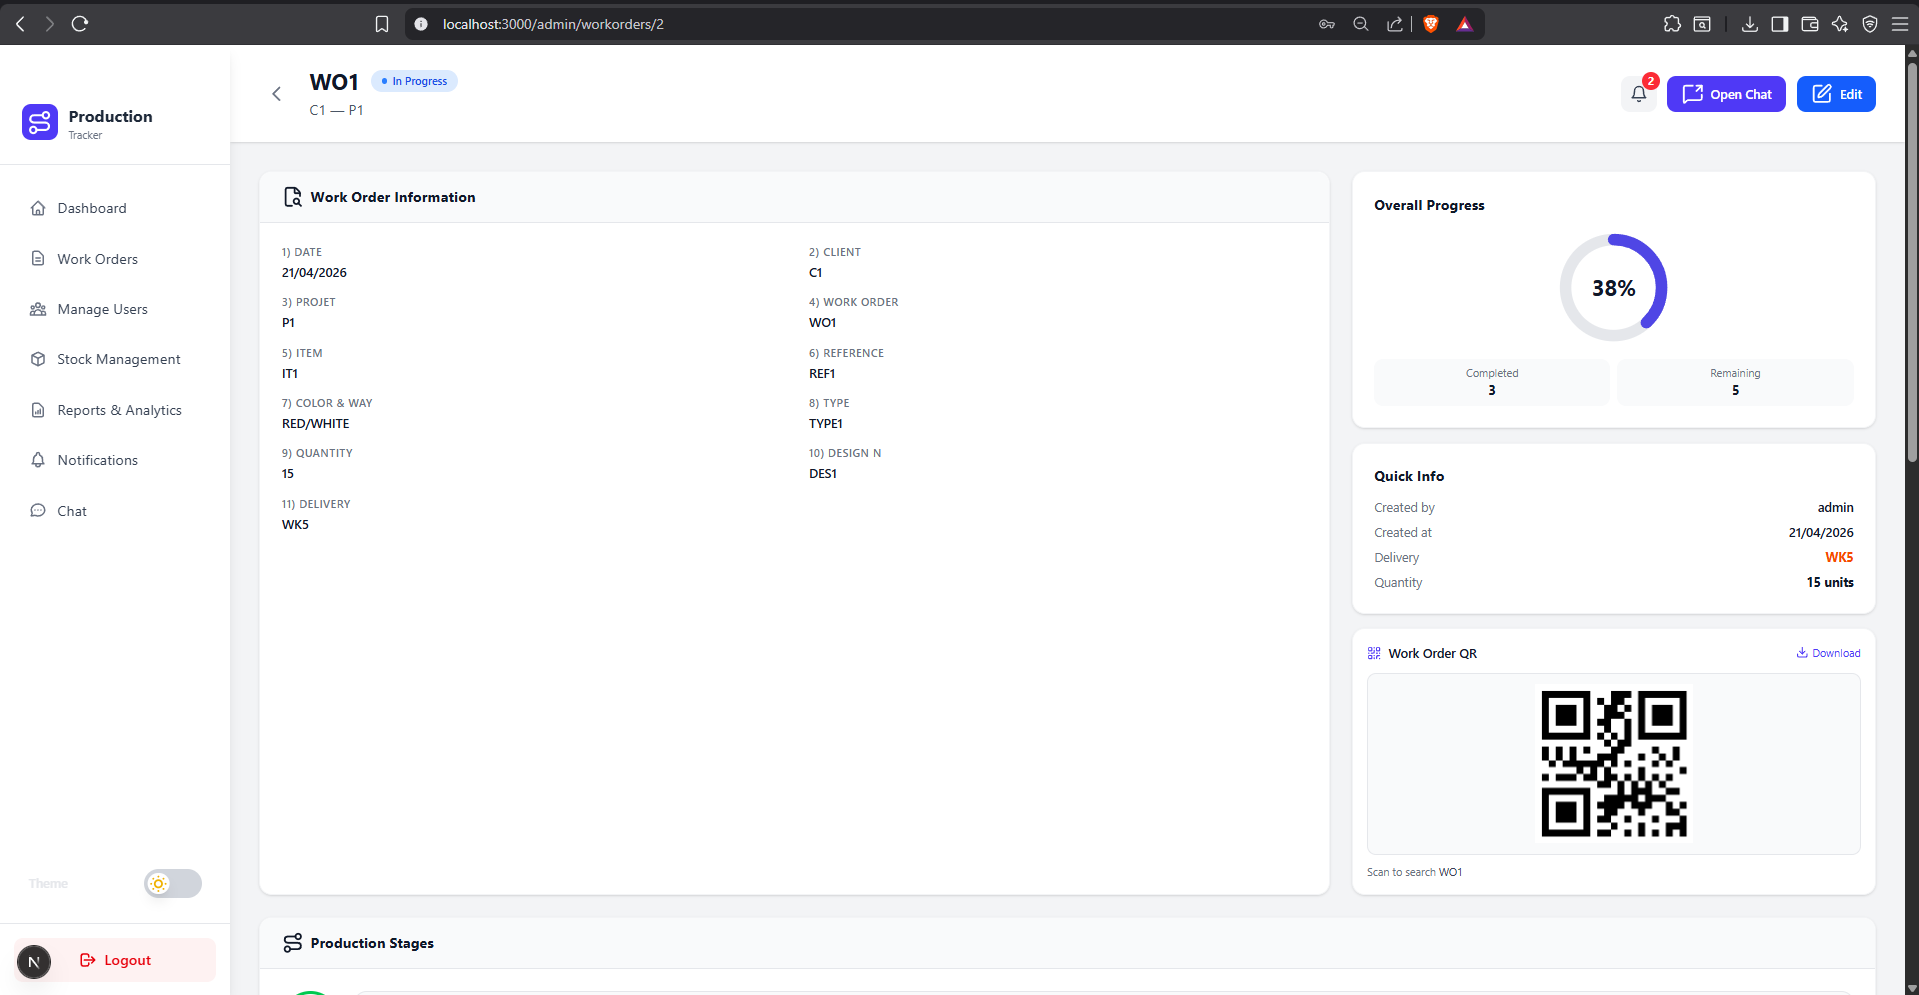
\includegraphics[width=\textwidth,keepaspectratio]{pictures/workorder detailes interface with QR code.png}
        \caption{Work Order Details Interface with QR Code}
        \label{fig:workorder-details-with-qr}
    \end{minipage}
    \hfill
    \begin{minipage}[t]{0.48\textwidth} 
        \centering
        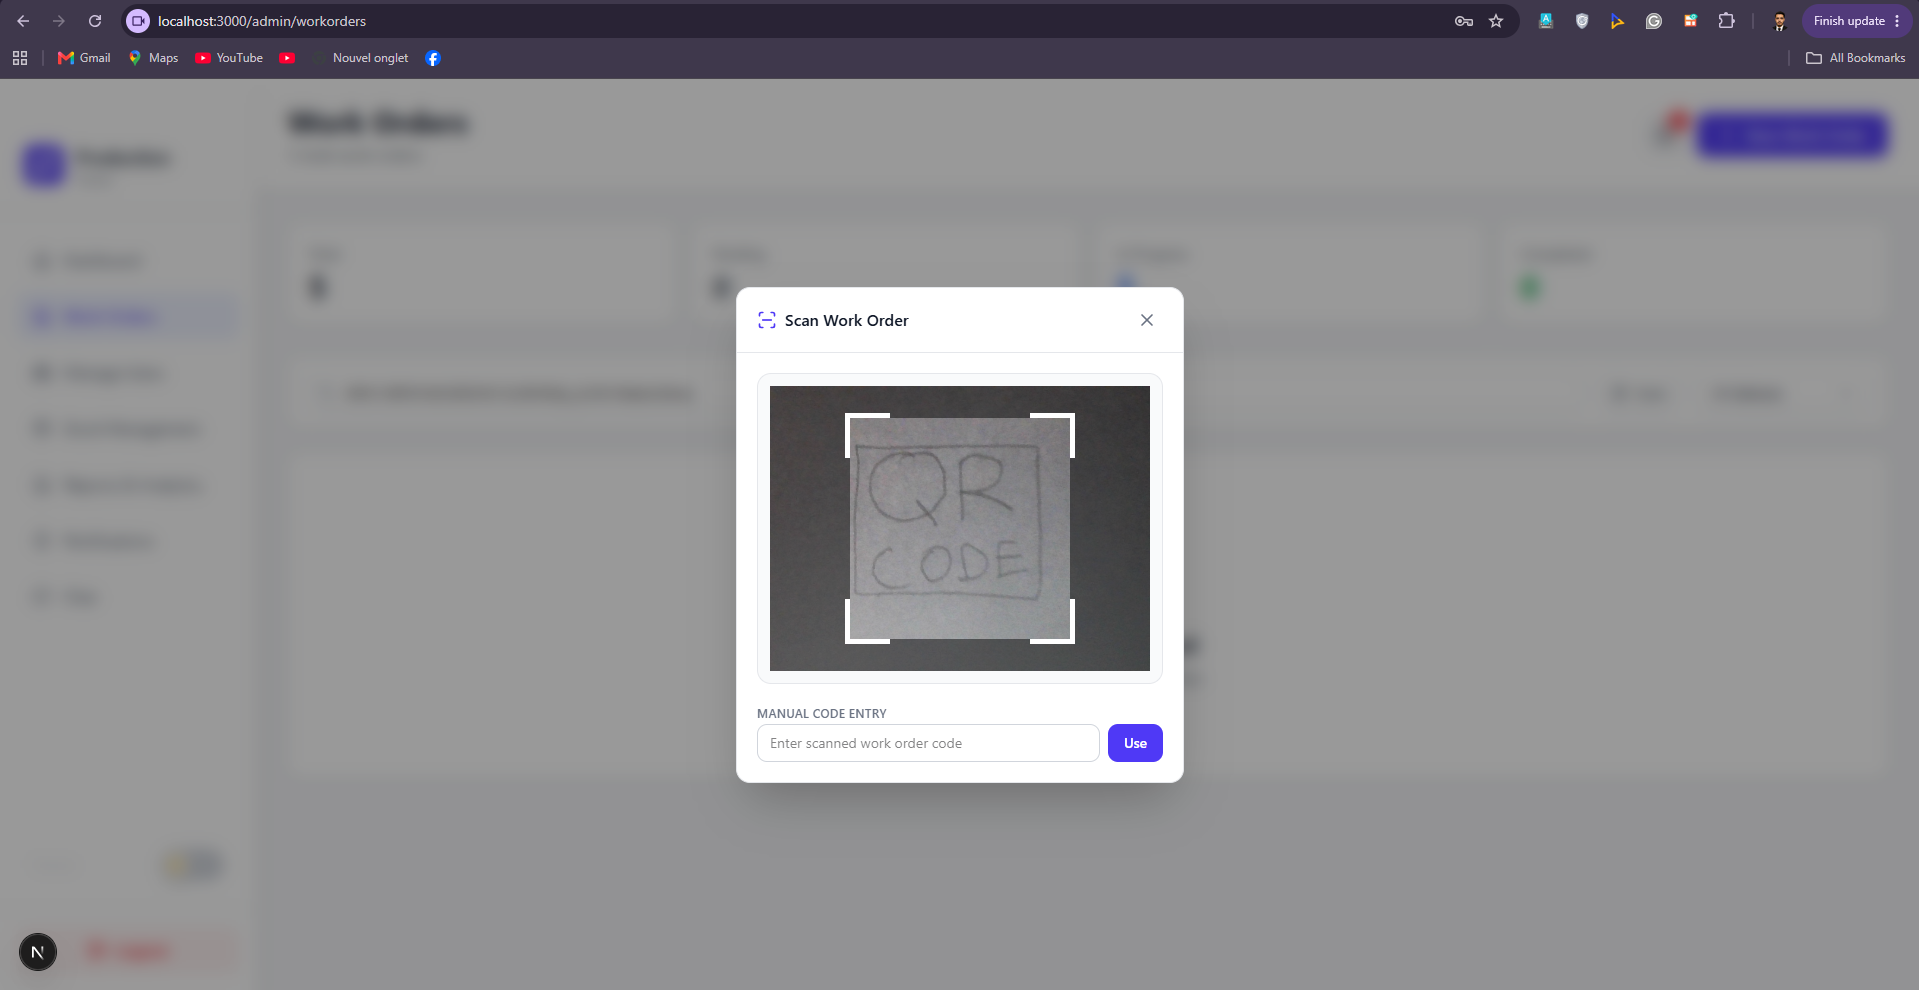
\includegraphics[width=\textwidth,keepaspectratio]{pictures/Qr code scanner interface.png}
        \caption{QR Code Scanner Interface}
        \label{fig:qr-code-scanner}
    \end{minipage}

\end{figure}
the figures \ref{fig:ai-report-interface} and \ref{fig:analytics-dashboard} provide an overview of the AI report interface and the analytics dashboard, respectively. The AI report interface allows administrators to generate and view AI-assisted reports, while the analytics dashboard provides visualizations and insights based on production data for informed decision-making.
\begin{figure}[H]
    \centering

    \begin{minipage}[t]{0.48\textwidth}
        \centering
        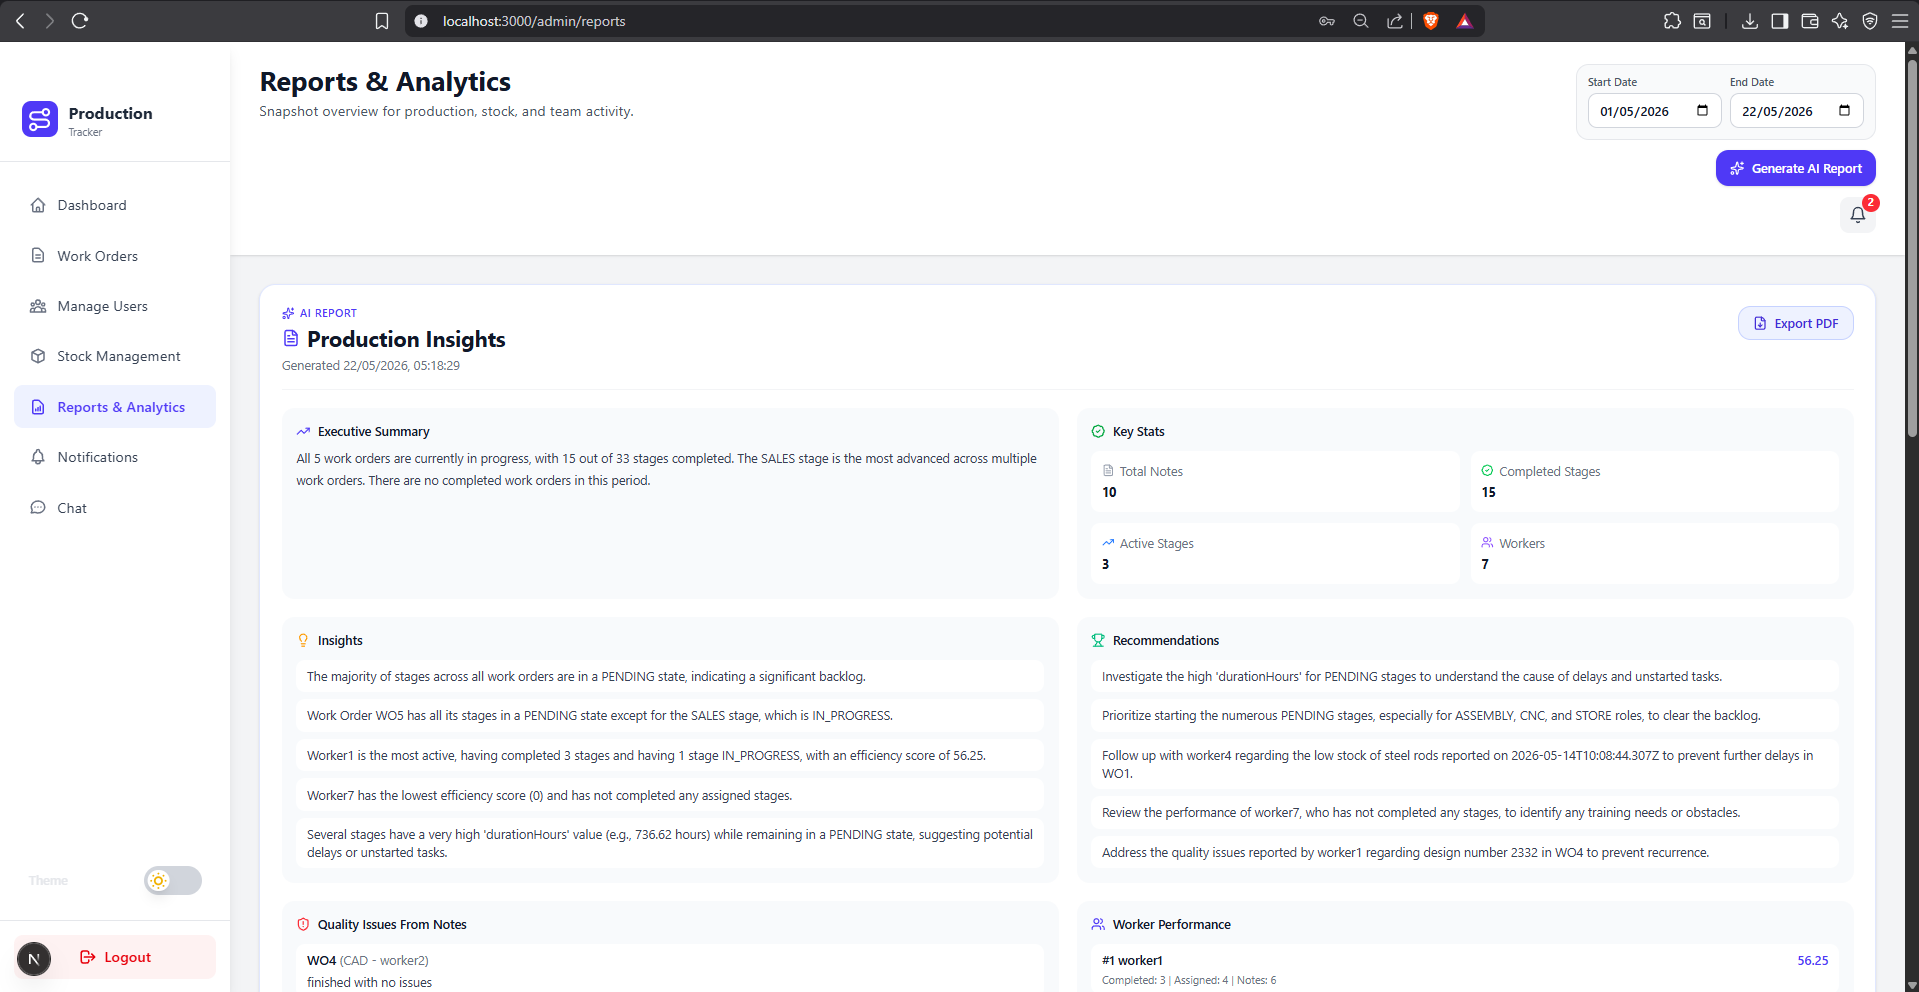
\includegraphics[width=\textwidth,keepaspectratio]{pictures/Ai report interface.png}
        \caption{AI Report Interface}
        \label{fig:ai-report-interface}
    \end{minipage}
    \hfill
    \begin{minipage}[t]{0.48\textwidth}
        \centering
        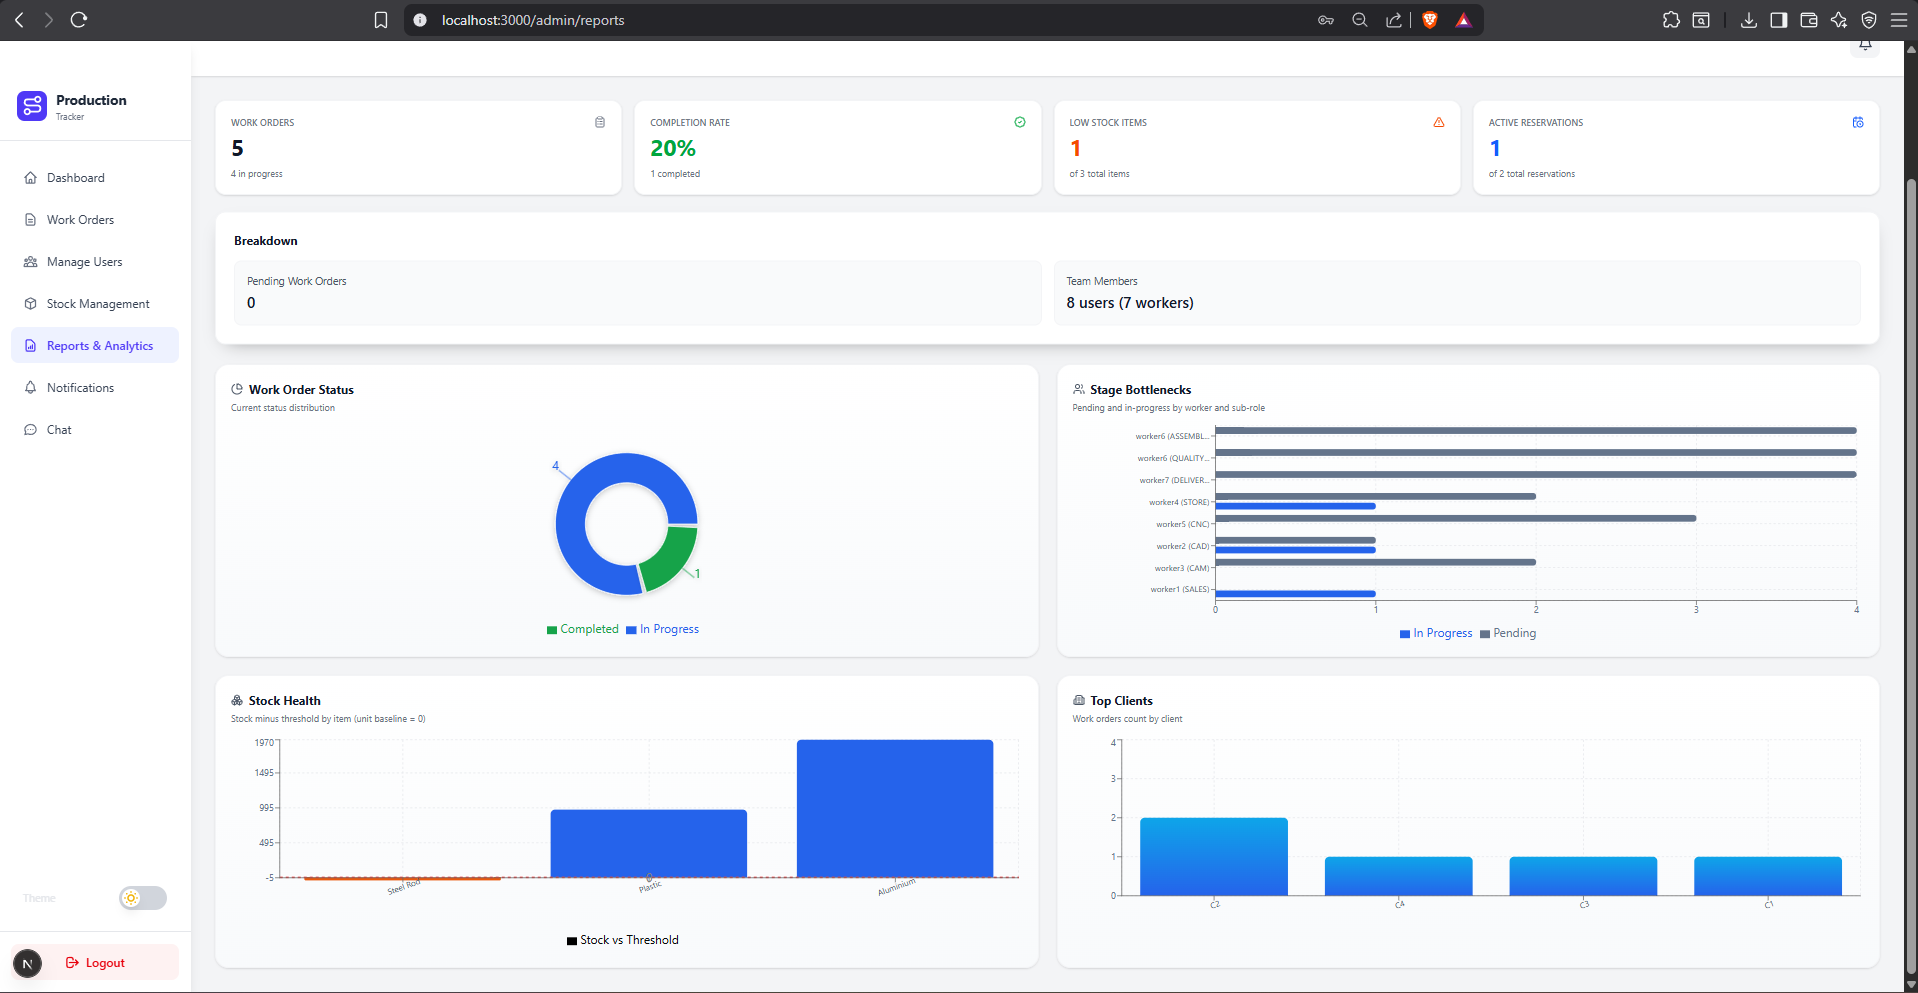
\includegraphics[width=\textwidth,keepaspectratio]{pictures/analytics Dashboard.png}
        \caption{Analytics Dashboard}
        \label{fig:analytics-dashboard}
    \end{minipage}

\end{figure}

\label{sec:sprint5-interfaces}

\section{Conclusion}
\label{sec:release2-conclusion}

Release 2 proved to be successful since it provided advanced functionalities that converted the Production Tracker into a fully-featured collaboration tool. The two sprints in Release 2 took 21 days each (summing up to 42 days), incorporating real-time communication features, effective identifying methods, and intelligent reporting. Combining Release 2 with Release 1 made up the 5-sprint process taking a total of 105 days to develop the application.


% Conclusion
\chapter*{General Conclusion}
\addcontentsline{toc}{chapter}{General Conclusion}

This end-of-studies project was driven by a real operational need at KTS: replacing a paper-based production tracking process with an integrated digital platform. Over the course of this report, we progressed from problem analysis to technical design and then to the practical implementation of a web application designed to better structure daily production activities and improve coordination among stakeholders.

The developed solution, \textbf{Production Tracker}, addresses the core business workflows identified during the analysis phase. It provides role-based authentication, work order management across the main production stages, stock monitoring and reservation, real-time notifications, and instant communication through chat. By bringing these functions together in a single system, the platform reduces information dispersion, limits manual errors, and improves the traceability of production operations.

From a technical perspective, the chosen stack (Next.js, Node.js/Express, PostgreSQL, Prisma, and Socket.IO) proved well aligned with the project objectives. It made it possible to build a modular architecture, ensure a clear separation of responsibilities between frontend and backend, and develop both transactional and real-time features efficiently. The resulting system offers a solid foundation for maintainability and future evolution.

Beyond the technical implementation, this work brings clear organizational value to the host company. Administrators now have better visibility over production progress, workers receive clearer task guidance, and communication delays are reduced through shared real-time information. In this way, the project contributes directly to KTS's digital transformation effort and supports more reliable day-to-day decision making.

Like any first complete version, the current platform can still be improved. Future work may include advanced analytics dashboards, richer KPI reporting, tighter integration with ERP systems, mobile-first access for shop-floor usage, and additional automation for planning and forecasting. These extensions would strengthen strategic monitoring while preserving the operational gains already achieved.

In conclusion, this internship project turned a real industrial problem into a functional and scalable software solution. It also marked an important personal and professional milestone, bringing together software engineering practices, system design, and iterative delivery in a real business context.


% References
\newpage
\chapter*{References}
\addcontentsline{toc}{chapter}{References}

\begin{enumerate}[label={[\arabic*]},leftmargin=*]
    \item \label{ref:MESdefinition} \textbf{Manufacturing Execution System (MES) Definition} --- Wikipedia.
    \url{https://en.wikipedia.org/wiki/Manufacturing_execution_system}

    \item \label{ref:KTSintro} \textbf{KTS (Kabelbaum Test Systems) intoduction} .
    \url{https://www.ktsistem.com/kurumsal.php?dl=en}

    \item \label{ref:KTSlogo} \textbf{KTS (Kabelbaum Test Systems) Logo} .
    \url{https://ktsistem.com/kurumsal.php?dl=en}
    
    \item \label{ref:SMOFT} \textbf{SMOFT ERP Official Website}.
    \href{https://www.smoft.io}{https://www.smoft.io}

    \item \label{ref:SMOFT-LOGO} \textbf{SMOFT ERP LOGO}.
    \url{https://www.facebook.com/smofterp/}

    \item \label{ref:SAPDM} \textbf{SAP Digital Manufacturing}.
    \href{https://www.sap.com/products/scm/digital-manufacturing.html}{SAP Digital Manufacturing official page}

    \item \label{ref:SAPDM-LOGO} \textbf{SAP Digital Manufacturing Logo}.
    \href{https://www.linkedin.com/posts/manoelfranklin_unlock-the-power-of-sap-digital-manufacturing-activity-7114950720767836161-D_I9}{SAP Digital Manufacturing logo}

    \item \label{ref:SAPDM-DASHBOARD} \textbf{SAP Digital Manufacturing Dashboard}.
    \href{https://www.sap.com/products/scm/digital-manufacturing.html}{SAP Digital Manufacturing official page}

    \item \label{ref:scrumguide} \textbf{The Scrum Guide} --- Scrum Guides. 
    \url{https://scrumguides.org/}

    \item \label{ref:scrum-Process} \textbf{The Scrum Process}  
    \url{https://www.pm-partners.com.au/insights/the-agile-journey-a-scrum-overview/}

    \item \label{ref:nextjs} \textbf{Next.js Documentation}.
    \url{https://nextjs.org/docs}

    \item \label{ref:nodejs} \textbf{Node.js Official Website}.
    \url{https://nodejs.org/en}

    \item \label{ref:express} \textbf{Express Official Website}.
    \url{https://expressjs.com/}

    \item \label{ref:postgresql} \textbf{PostgreSQL About Page}.
    \url{https://www.postgresql.org/about/}

    \item \label{ref:prisma} \textbf{Prisma ORM Documentation}.
    \url{https://www.prisma.io/docs/orm/overview/introduction/what-is-prisma}

    \item \label{ref:socketio} \textbf{Socket.IO Documentation (v4)}.
    \url{https://socket.io/docs/v4/}

    \item \label{ref:vscode} \textbf{Visual Studio Code Official Website}.
    \url{https://code.visualstudio.com/}

    \item \label{ref:diagramsnet} \textbf{diagrams.net Documentation - wikipedia}.
    \url{https://en.wikipedia.org/wiki/Diagrams.net}

    \item \label{ref:latex} \textbf{LaTeX Official Website}.
    \url{https://www.latex-project.org/}

    \item \label{ref:jwt} \textbf{JSON Web Token (JWT)}.
    \url{https://en.wikipedia.org/wiki/JSON_Web_Token}
\end{enumerate}


% ==================== BIBLIOGRAPHY ====================
\bibliographystyle{plain}
%\bibliography{references}

% ==================== APPENDICES ====================
\appendix


\end{document}